%%%%%%%%%%%%%%%%%%%%%%%%%%%%%%%%%%%%%%%%%%%%%%%%%%%%%%%%%%%%%%%%%%%%%%%%%%%%
%%%%%%% To toogle between Marketing Science / INFORMS format, 
%%%%%%% search for: %MKSC_FORMAT% 
%%%%%%%
%%%%%%%%%%%%%%%%%%%%%%%%%%%%%%%%%%%%%%%%%%%%%%%%%%%%%%%%%%%%%%%%%%%%%

%%%%%%%%%%%%%%%%%%%%%%%%%%%%%%%%%%%%%%%%%%%%%%%%%%%%%%%%%%%%%%%%%%%%%%%%%%%%
%% Author template for Marketing Science (mksc)
%% Mirko Janc, Ph.D., INFORMS, mirko.janc@informs.org
%% ver. 0.95, December 2010
%%%%%%%%%%%%%%%%%%%%%%%%%%%%%%%%%%%%%%%%%%%%%%%%%%%%%%%%%%%%%%%%%%%%%%%%%%%%
% %\documentclass[mksc,blindrev]{informs3} % current default for manuscript submission

%MKSC_FORMAT% 
\documentclass[nonblindrev]{informs3}
%\documentclass[a4paper,11pt]{article}


%MKSC_FORMAT% 
\OneAndAHalfSpacedXI % current default line spacing
% %\OneAndAHalfSpacedXII
% %%\DoubleSpacedXII
% %%\DoubleSpacedXI




% If hyperref is used, dvi-to-ps driver of choice must be declared as
%   an additional option to the \documentclass. For example
%\documentclass[dvips,mksc]{informs3}      % if dvips is used
%\documentclass[dvipsone,mksc]{informs3}   % if dvipsone is used, etc.

% Private macros here (check that there is no clash with the style)
%  \usepackage{subcaption}
% Natbib setup for author-year style
\usepackage{natbib}
 \bibpunct[, ]{(}{)}{,}{a}{}{,}%
 \def\bibfont{\small}%
 \def\bibsep{\smallskipamount}%
 \def\bibhang{24pt}%
 \def\newblock{\ }%
 \def\BIBand{and}%

\usepackage{algorithm}
\usepackage{algorithmicx}
\usepackage{algpseudocode}
\usepackage{subfig}
\usepackage{amsmath,graphicx,amssymb}


\setlength{\parindent}{1cm} % Default is 15pt.

%% Setup of theorem styles. Outcomment only one. 
%% Preferred default is the first option.

%MKSC_FORMAT%  \TheoremsNumberedThrough     % Preferred (Theorem 1, Lemma 1, Theorem 2)
%MKSC_FORMAT% \TheoremsNumberedByChapter  % (Theorem 1.1, Lema 1.1, Theorem 1.2)

%% Setup of the equation numbering system. Outcomment only one.
%% Preferred default is the first option.
% \EquationsNumberedThrough    % Default: (1), (2), ...
%\EquationsNumberedBySection % (1.1), (1.2), ...



%MKSC_FORMAT% \DeclareMathOperator{\logit}{logit}
\newcommand{\logit}{logit}

% to use for comments
\newcommand{\alexander}[1]{\textcolor{blue}{\textbf{(alexander)} #1}}
\newcommand{\eric}[1]{\textcolor{red}{\textbf{(eric)} #1}}
% ==============
% use for naming algorithms: easier to change later
%
\newcommand{\fixedexpress}{\textbf{express}} 

% previously referred to as greedy
% we need to global change: greedy -> \egreedy
\newcommand{\egreedy}{$\epsilon$-\textbf{greedy}} 


% previously referred to as greedythres
% we need to global change: greedythres -> \egreedythres
\newcommand{\egreedythres}{$\epsilon$-\textbf{greedythres}} 

\newcommand{\mismin}{\textbf{max-misclass}} 

\newcommand{\ts}{\textbf{TS} } 

\newcommand{\edts}{$\epsilon$-$\delta$-\textbf{diffuse TS} } 

% previously referred to as TSregthres
\newcommand{\tsthres}{\textbf{TS-thres} } 

% previously referred to as TSthres
\newcommand{\edtsthres}{$\epsilon$-$\delta$-\textbf{TS-thres} } 
\newcommand{\uncert}{\textbf{max-uncert} } 


\newcommand{\fixedexpressS}{\textbf{exp}} 

% previously referred to as greedy
% we need to global change: greedy -> \egreedy
\newcommand{\egreedyS}{$\epsilon$-\textbf{g}} 


% previously referred to as greedythres
% we need to global change: greedythres -> \egreedythres
\newcommand{\egreedythresS}{$\epsilon$-\textbf{g-thr}} 

\newcommand{\misminS}{\textbf{max-mis}} 

\newcommand{\tsS}{\textbf{TS} } 

\newcommand{\edtsS}{$\epsilon$-$\delta$-\textbf{dif TS} } 

% previously referred to as TSregthres
\newcommand{\tsthresS}{\textbf{TS-thr} } 

% previously referred to as TSthres
\newcommand{\edtsthresS}{$\epsilon$-$\delta$-\textbf{TS-thr} } 
\newcommand{\uncertS}{\textbf{uncert} } 
%% Notation in this paper %%
% S - a set of items in a questions
% |S| - number of items per question
% N- number of respondents
% L - items per respondent
% J - question sper respondent
% m - number of total items
% b - batch size

\newcommand{\numitems}{n} 
\newcommand{\numtopset}{k} 
\newcommand{\numperset}{L} 
\newcommand{\topset}{\text{Top}_k} 

\newcommand{\titleofthispaper}{
	\textbf{Active Learning for Ranking and Selection: \\
	Idea Screening with Bandit MaxDiff} 
}
%{Bandit MaxDiff: Best-Item Identification for Large-Scale Idea Screening} 

%%%%%%%%%%%%%%%%
\begin{document}
%%%%%%%%%%%%%%%%

% Cover Page
\begin{center}

	~ \\

	\vspace{2in}

	\titleofthispaper

	\vspace{1in}

	{Eric Schwartz,}
	\emph{University of Michigan, {ericmsch@umich.edu} } \\
	{Kenneth Fairchild,} 
	\emph{Sawtooth Software} \\
	{Bryan Orme,}
	\emph{Sawtooth Software} \\
	{Alexander Zaitzeff,}
	\emph{University of Michigan} 

	\vspace{1in}

	%Date
	\today
	%January 31, 2018


\end{center}


% Outcomment only when entries are known. Otherwise leave as is and 
%   default values will be used.
%\setcounter{page}{1}
%\VOLUME{00}%
%\NO{0}%
%\MONTH{Xxxxx}% (month or a similar seasonal id)
%\YEAR{0000}% e.g., 2005
%\FIRSTPAGE{000}%
%\LASTPAGE{000}%
%\SHORTYEAR{00}% shortened year (two-digit)
%\ISSUE{0000} %
%\LONGFIRSTPAGE{0001} %
%\DOI{10.1287/xxxx.0000.0000}%

% Block of authors and their affiliations starts here:
% NOTE: Authors with same affiliation, if the order of authors allows, 
%   should be entered in ONE field, separated by a comma. 
%   \EMAIL field can be repeated if more than one author

% \ARTICLEAUTHORS{%
% \AUTHOR{Eric Schwartz}
% \AFF{University of Michigan, \EMAIL{ericmsch@umich.edu}, \URL{}}
% \AUTHOR{Alexander Zaitzeff}
% \AFF{University of Michigan, \EMAIL{azaitzef@umich.edu}, \URL{}}
% \AUTHOR{Kenneth Fairchild}
% \AFF{Sawtooth Software, \EMAIL{}, \URL{}}
% \AUTHOR{Bryan Orme}
% \AFF{Sawtooth Software, \EMAIL{}, \URL{}}

% % Based on an earlier 2015 Sawtooth Conference Paper \\ with Kenneth Fairchild, Bryan Orme, Eric Schwartz.
% } % end of the block


% Author's names for the running heads
% Sample depending on the number of authors;
% \RUNAUTHOR{Jones}
% \RUNAUTHOR{Jones and Wilson}
% \RUNAUTHOR{Jones, Miller, and Wilson}
% \RUNAUTHOR{Jones et al.} % for four or more authors
% Enter authors following the given pattern:
%MKSC_FORMAT% 
\RUNAUTHOR{Schwartz et al.}

% Title or shortened title suitable for running heads. Sample:
% \RUNTITLE{}
% Enter the (shortened) title:
%MKSC_FORMAT% 
\RUNTITLE{Bandit MaxDiff}


% Full title. Sample:
% \TITLE{Bundling Information Goods of Decreasing Value}
% Enter the full title:
%\titleofthispaper \\
%MKSC_FORMAT% 
\TITLE{Active Learning for Ranking and Selection in Marketing: Efficient Idea Screening with Bandit MaxDiff}


\vspace{1mm}
	% OLD TITLES

	% Best-Arm Identification for Choice Experiments: \\ Applications to Large-Scale Adaptive MaxDiff \\
	% and Idea Screening \\

	%{\\Technical Appendix for ISMS Practice Prize}



%MKSC_FORMAT% 
\ABSTRACT
%\textbf{Abstract:}
{% % Enter your abstract
Marketing research often measures consumers' preferences to identify what they consider most important items among many candidates, such as product benefits, innovative features, or message appeals. While the objective of existing methods is typically to estimate parameters representing all preferences, these problem settings call for a different pair of potential goals: minimize the cost of correctly select the best items while ensuring high the accuracy and precision of estimated preferences for the best items. This goal is especially important in settings with extremely large numbers of items. Common techniques for identifying preferences are idea screening and choice tasks, including conjoint analysis and maximum-difference (MaxDiff) scaling, however, are not built for large-scale problems, like identifying the best dozen items out of hundreds. This research proposes a new approach, rooted in active learning and multi-armed bandit algorithms from statistical machine learning, to overcome this scale and make goal-directed adaptive ranking and selection problems more efficient. Using MaxDiff as an illustration of the broader class of problems, the research proposes a new approach: Bandit MaxDiff. The empirical studies shows Bandit MaxDiff can increase efficiency four-fold over standard MaxDiff scaling by identifying the most influential preferred items with fewer survey respondents. The proposed solution use information from initial respondents, so later respondents receive designs oversampling the items most likely to be the in the overall top set. Instead of learning all preference parameters with equal precision, Bandit MaxDiff estimates the parameters of most interest to the respondent with more precision. The methods are implemented empirically using multiple MaxDiff surveys: one from Proctor \& Gamble, consumer packaged goods manufacturer, and various synthetic datasets. Through a series of simulation experiments, a range of benchmark algorithms are considered to illustrate under what conditions the proposed approach out performs existing methods. The researchers' approach draws on both the classic multi-armed bandit literature, active learning in statistical machine learning, and recent work on the best k-arm identification problem. Several new components, which can apply outside the idea screening and preference measurement problem, are introduced to the algorithms to (a) control robustness in a changing environment when using Thompson Sampling, (b) allow the algorithms to learn an unranked (versus ranked) top set, and (c) evaluate a set of approximations to posterior sampling to allow faster model updates.

} ~ \\


% Fill in data.


%MKSC_FORMAT% 
\KEYWORDS
%\textbf{Keywords:}
{idea screening, maximum-difference surveys, MaxDiff, adaptive conjoint, active learning, multi-armed bandit, best arm identification, Bayesian bootstrap, best-worst scaling, Thompson Sampling, uncertainty minimization}



%\textbf{Outdated Abstract, see Introduction.} For large MaxDiff studies whose main purpose is identifying the top few items for the sample, a new adaptive approach called Adaptive MaxDiff may increase efficiency fourfold over standard non-adaptive MaxDiff.  Adaptive MaxDiff leverages information from previous respondents via aggregate logit and Thompson Sampling so later respondents receive designs that oversample the topmost items that are most likely to turn out to be the overall winners. Our approach applies beyond MaxDiff problems to a more general set of bandit problems. We propose a flexible algorithm, $\epsilon$-Diffuse Thompson Sampling (TS), which nests traditional TS. Blending ideas from $\epsilon$-greedy in machine learning and Bayesian approaches, this is a more robust version of TS, which a manager can control with tuning parameters. For instance, being less risk averse, one may drawn more items from diffuse posteriors, making the algorithm robust to changing environments, even extreme non-stationarity. We implement the methods using MaxDiff survey from a large consumer packaged goods manufacturer. Beyond showing our approach outperforms better than current methods, we show under which conditions it performs even better than (larger problems) or just as well as existing methods (smaller problems).

%MKSC_FORMAT%  
\maketitle



%%%%%%%%%%%%%%%%%%%%%%%%%%%%%%%%%%%%%%%%%%%%%%%%%%%%%%%%%%%%%%%%%%%%%%

% Samples of sectioning (and labeling) in MKSC
% NOTE: (1) \section and \subsection do NOT end with a period
%       (2) \subsubsection and lower need end punctuation
%       (3) capitalization is as shown (title style).
%
%\section{Introduction.}\label{intro} %%1.
%\subsection{Duality and the Classical EOQ Problem.}\label{class-EOQ} %% 1.1.
%\subsection{Outline.}\label{outline1} %% 1.2.
%\subsubsection{Cyclic Schedules for the General Deterministic SMDP.}
%  \label{cyclic-schedules} %% 1.2.1
%\section{Problem Description.}\label{problemdescription} %% 2.


\newpage

% ASK GUI LIBERALI HOW TO CITE 2015 SAWTOOTH PAPER

\section{Introduction}

Firms measure consumers' preferences to identify the characteristics most important to them among a set of candidates, such as, product benefits, new features, or message appeals. For instance, consider the following managerial decisions:

\begin{itemize}
	\item \emph{Crowd-sourced feature selection.} Technology companies have long invited consumers to provide ideas for new products and improvements. For example, automotive companies offer complex products, such as self-driving cars, with different bundles of hundreds of possible features. Consumer surveys reveal the most preferred features to help the firms decide which should be included on each model.
	\item \emph{Product assortment offerings.} Retailers can respond quickly to demand and consumer preferences by changing their product offerings. In anticipation of a new fashion season, an e-commerce retailer might survey customers to identify preferred styles and lines and select the range of items to make available.
	\item \emph{Marketing communications.} As products are developed, firms must decide which consumer benefits to emphasize. Consumer packaged goods companies use marketing research to determine which product claims should be central to an advertising campaign and shown on packaging. Out of hundreds of potential benefits, they must select a handful for marketing messages.
\end{itemize}

These problems share a common challenge to identify the best items out of many facing uncertainty and limited resources. These problems call for a manager to output a list of top items in one of two forms: (A) select the highest ranked top set (unordered) or (B) select the top set and rank the items within the set (ordered). With all of the resources and time, these problems are solved with more data. But in practice, data collection is costly, so there is a desire to solve these problems by using data, such as actual customer surveys, more efficiently.  Therefore, managers seek to increase the information gained per dollar spent on survey respondents. 

This research puts forward a family of adaptive data collection methods. While these are rooted in the statistical machine learning literatures, including Thompson Sampling \citep{thompson1933likelihood}, our methods are heuristics that we show to have strong empirical performance because they are comprised of new components proposed here. Among these novel adaptive sampling extensions are: 
%(1) sampling from a finite mixture of two posteriors (instead of one), balance exploration versus exploitation to be more robust in practice; (2) selecting to observe items with maximum expected loss based on Bayesian decision theory, but done efficiently using approximate posterior sampling; and (3) thresholding by oversampling items close to the decision boundary. 
\begin{itemize}
\item (1) sample the item that maximizes \emph{conditional minimized Bayes risk}, efficiently using approximate posterior sampling; 
\item (2) oversample items close to a \emph{threshold}, the decision boundary; and 
\item (3) sample from a mixture of posteriors (regular one and a more diffuse distribution) to making the exploration-exploitation balance more robust in practice.
\end{itemize}
We consider the methods' performance relative to each other and against benchmarks. All the algorithms follow the same broad steps of our general adaptive approach (Algorithm \ref{alg:general}).

While our approach is general, we illustrate an application to one instance in the class of analogous problems, idea screening for large numbers of items using consumer preference measurement with maximum-difference scaling, a form of best-worst scaling preference measurement in which consumer respondents select their most and least preferred alternatives from a set. 

To do this, we instantiate our framework in this setting, proposing, \emph{Bandit MaxDiff}. We demonstrate that this new method is the best-performing available adaptive MaxDiff, in particular, for large numbers ideas. While idea screening methods typically involve preference measurement surveys, such as choice-based conjoint and MaxDiff, they are designed for measuring preferences among, say, 20 ideas, but are not built for large-scale problems, like identifying the best set of 20 ideas out of 100 alternatives. Yet as managers push preference measurement methods into a larger scale, market researchers must collect data from more respondents via surveys or more involved interviews, increasing costs, especially if those respondents are actual customers.

We illustrate the Bandit MaxDiff approach empirically through a suite of simulations based on other MaxDiff and with an in-market live test. Working with Procter \& Gamble (P\&G), we show the new method can increase efficiency 2.5 to 4 times over current MaxDiff practices by accurately identifying the best items more quickly with fewer respondents. Developed in collaboration Sawtooth Software, Bandit MaxDiff is shown to cut costs for large MaxDiff studies conducted to identify respondents’ most preferred items, allowing the potential savings of millions of dollars in market research budgets. 

We provide evidence of implementing the approach in real-time with P\&G. Compared to the firm's standard approaches to ranking and selection problems, P\&G witnessed a 240\% increase in efficiency in a live, in-market head-to-head randomized-controlled experiment. We provide evidence via simulations with up to 400\% improvement; the approach appears to be applicable to other firms facing similar problems. The simulation studies use multiple past MaxDiff surveys administered by P\&G to analyze the range of potential savings and how different conditions lead to more modest or extreme savings.

How much cost savings could a company like P\&G experience using our new approach? Consider the cost of a typical online data collection effort. Costs to develop customized consumer target segments can range from \$6 to \$18 per completed consumer sample task. For a large study analyzing 50 to 150 or more possible preferences, desired sample sizes are usually between 1,000 and 3,000 respondents, meaning each survey costs \$18,000 to \$54,000. Bandit MaxDiff can decrease the required sample size by 2 to 4 times. With sample size savings of 500 to 2,000 respondents, cost savings could be in the range of \$3,000 to \$36,000.

Like the problem that Bandit MaxDiff resolves, the broader class of problems, which the methodology in this paper addresses, is characterized by the following elements:
\begin{itemize}
\item \emph{Limited budget.} Surveys target customers carries a high opportunity cost to asking them about ideas that do not help finding the most preferred ones.
\item \emph{Loss function.} The market researcher's ultimate decision (e.g., selecting the most preferred ideas) is linked to learning their relative ranking and/or preference values, directly.
\item \emph{Sequential data collection.} Data from past respondents can be used to determine what to ask the next respondent.
\item \emph{Pool of ideas.} The decision-maker knows all possible ideas up-front and selects which ask respondents about next.
\item \emph{Stochastic output.} After asking respondents about ideas, the revealed preference is a noisy signal of true preference.
\end{itemize}

\begin{algorithm}
\caption{Sketch of Adaptive Data-Collection} \label{alg:general}
\begin{algorithmic}[1]
\State Initialize with a uniform sample.
\While {Stopping rule not satisfied:} 
\State Collect new data for selected items.
\State Update model estimates and characterize uncertainty.
\State Select items for next round.
\EndWhile
\end{algorithmic}
\end{algorithm}

The specific proposed approach builds on algorithms initially developed and commonly used for \emph{multi-armed bandit} problems in the marketing literature \citep{HauserEtAl2009,schwartzetal2017,Scott2010,urban2013morphing}. The traditional bandit problem epitomizes the "earning while learning" challenge, which seeks to identify the best way to allocate fixed resources to competing alternatives while maximizing gains. Our problem departs from the standard bandit challenge and requires updates to the known algorithms.

But the problem we address is more aligned with the related \emph{best arm identification} \citep{russo2016simple}. While the traditional bandit problem accumulates maximum reward for the researcher throughout all rounds $1$ to $T$ (i.e., it identifies items delivering the most sales/clicks/etc.), in best arm identification, the goal is to correctly select the best arm (or subset of best $k$ arms) out of all only in the final round $T$. Since thee marketer derives no reward for the initial rounds, best arm identification is known as a \emph{pure learning} problem, as opposed to the typical bandit problem which is an \emph{earning while learning} problem

A generalization of the best $k$ arm identification problem is known as the \emph{ranking and selection}, in which the decision maker tries to learn the true ranking of all items or a subset of items to choose the most preferred option. The problem typically does not necessarily involve sequential data collection and does not feature stochastic observations, but both features can appear in variants.

Sequential ranking and selection problems often appear in the field of active learning \citep{balcan2009agnostic,dasgupta2008general}. While established in the theoretical statistics and machine learning literature, active learning rarely appears in marketing studies. One exception is \citep{dzyabura2011activelearn}, in which active learning algorithms are considered as decision-making heuristics for individual consumers. 

Active learning algorithms are typically assumed to be deterministic observations for the sequential problem of ranking and selection. Labels are revealed with certainty and do not have to be revisited. In stochastic ranking and selection problems, the observations are values sampled from a distribution with unknown parameters.

Surprisingly, only recently the literature has made explicit links between the \emph{active learning}, \emph{best arm identification}, and \emph{multi-armed bandit problems}. \cite{gantigray2013}, for example, ... b


Our problem is a sequential stochastic ranking and selection problem. We also consider circumstances in which ranking does not matter within the selected subset, which is characterized by the best k-arm identification problem. The framework we employ therefore draws on both the active learning and multi-armed bandit methods.

We also consider the practical implementation of the three algorithms, including their scalability and speed. We provide alternative, faster versions that may sacrifice theoretical statistical validity. Some fast heuristics, however, perform well.



To illustrate the effectiveness of Bandit MaxDiff, we first formalize our problem and the general framework to be used. We highlight the framework's active learning and bandit components, relating it to the marketing and statistical machine learning literature. After formalizing the discrete choice model for analyzing MaxDiff data, we introduce Bandit MaxDiff as a particular instance of the broader algorithm. We then present our empirical results in the standard setting, as well as variants of the main results. We implement the methods using a MaxDiff survey administered by Sawtooth Software and P\&G. 



\eric{ending new intro here}

 -- the selection and the selection with ranking -- 

In this paper, we develop a new method to solve large-scale idea screening challenges that decreases expenses and increases information gained per dollar spent on surveys. The method, Bandit MaxDiff, uses algorithms from multi-armed bandit literature and active learning for ranking and selection problems from the computer science field. 






% ---- 
% new intro should continue from here.



% Facing this problem, firms such as Proctor \& Gamble (P\&G) often turn to MaxDiff surveys to screen out weaker ideas, identify the best items, and learn more about them. Among all corporate users of the market research software, Sawtooth Software, 70\% of them have used MaxDiff in 2017. This data collection and preference learning process can be made more efficient through adaptive methods. But this problem is not the same as that solved by other adaptive approaches, such as adaptive (choice-based) conjoint analysis, or ACA (ACBC) (Aurora and Huber 2002; Toubia et al. 2004) and preliminary adaptive MaxDiff approaches (Orme 2006). 

% But typical adaptive discrete choice experiment methods do not have the objective suited for this problem. Those methods seek to learn preferences for all items equally. Even the adaptive versions of conjoint, such as ACBC, serve respondents with optimized questions to minimize preference uncertainty everywhere and maximize the researcher's overall learning. By contrast, in our setting, we specifically want to learn how much respondents prefer certain items, such as the top 20 items, and do not need to spend resources learning how precisely the 100th-best item differs from the 90th-best item. 

% Further, if we were to employ standard MaxDiff or adaptive conjoint approaches here, they are inefficient at this scale and practically infeasible. The current implementations of MaxDiff would require many thousands of respondents, making the approach infeasible, inefficient, and costly. At best, marketing researchers often use pretest or screening phases to select a smaller set, which they then use for the main analysis. This approach can be inaccurate if it does not obtain enough information to identify (and rank) the high-scoring items by spreading sample sizes to thinly, or if it is accurate, it would be inefficient by spending too many respondents on low-scoring items. Yet there is no systematic method to smoothly transition out of that screening phase, even when the ultimate objective is to correctly identify (and rank) the set of most preferred items. There is limited marketing literature in idea screening (Toubia and Flores 2007), which we return to later.

% We frame this as a sequential decision making problem under uncertainty where the decision maker (market researcher) selects a set of items to serve to the next respondent. This is repeated over many respondents. When surveying is completed,  the set of items predicted to be the best is selected as a final decision: this is evaluated by the list's accuracy (hit rate as percent correct) and the cost required (number of respondents).


% Quick outline of flow:
% - P\&G and GM have a common problem: they want to find the best things out of a large set of ideas.
% - New kind of problem. 
% - Many people in industry are trying to solve this problem. 
% - This is like classic Idea Screening, but we have a new twist using best-arm identification and bandit algorithms for Adaptive MaxDiff. 
% - This isn't conjoint. 
% - This needs to be adaptive.
% - If it weren't adaptive, this would cost much more money. 



% Our proposed solution, Bandit MaxDiff, is a new form of MaxDiff that is adaptive utilizes multi-armed bandit algorithms. It is \emph{adaptive} because it uses information from previous respondents to decide what to show later respondents. In particular, later respondents receive survey designs that oversample the items that are most likely to turn out to be the in the overall top set. The \emph{bandit} component stems from the multi-armed bandit (MAB) methods we use to resolve the tradeoff between exploring the preferences for all items to learn which is best and exploiting the information we have collected from respondents so far by focusing on the items with preferences believed to be large so far. This is known as the explore-exploit tradeoff and is at the heart of the entire MAB literature. The MAB work in marketing typically is applied to optimization of advertising \citep{schwartzetal2017}, website design \citep{hauser2009website,scott2010modern,urban2013morphing}, or pricing (Misra et al. 2017). One benefit is that, instead of learning all preference parameters with equal precision, the Bandit MaxDiff more precisely estimates the parameters of most interest to the manager. 

% However, Bandit MaxDiff is not a simple application of existing MAB algorithms because our adaptive preference measurement setting differs from the canonical MAB problem in a number of ways. For a bandit problem, we would earn an observable reward, such as, click, acquisition, or purchase, immediately after each decision. While we have immediate observations (choice among a set), that is not our reward directly. Instead, our goal is to correctly identify the best items, which cannot even be evaluated in real-time during the data collection process.

% Yet that is exactly the objective of a lesser-known MAB problem variant: \emph{best-k-arm identification} multi-armed bandit problem. Identifying the best k arms of a set of arms has historically received less focus, but has recently attracted theoretical study in the computer science literature, described in the literature review (Gabillon et al 2012; Jamieson et al. 2014; Kalyanakrishnan et al. 2012; Kaufmann and Kalyanakrishnan 2013; Russo 2016). The recent attention is due to the increase in rigorous study of the practice of A/B testing in practice and adaptive experimentation at technology companies. The best arm identification problem is, in part, distinct because it is a pure exploration setting, whereas the canonical bandit calls for explore-exploit tradeoff. While both are adaptive, the explore-exploit problem deals with maximizing earning while learning, but the pure explore setting is just about learning during the data collection. 

% As this problem differs from the standard bandit setting, we make new methodological contributions. We introduce and test several new components to these algorithms. In particular, first, we introduce researcher-chosen parameters to control robustness to a changing environment when using Thompson Sampling. Our approach -- with the survey context in mind – differs because it prevents the case where the earliest respondents preferences, if they are not representative of the target population, from having an outsized influence on the questions for later respondents, hence, preserving the desired effectiveness. Second, we allow for the algorithms to specifically learn an unranked (or ranked) top set. And third, we evaluate a set of approximations to posterior sampling to allow for faster model updates. These three algorithmic innovations could also be applied apply outside of our idea screening and preference measurement problem.


% Although MaxDiff shares much in common with conjoint analysis, MaxDiff is not conjoint. Methodological advances, such as adaptive choice-based conjoint (ACBC), have long sought to improve efficiency, obtaining more information from fewer respondents. Those methods use past responses to select the next question to improve precision of all parameters. ACBC methods present respondents with questions to reduce the uncertainty where it is greatest. For example, the algorithm selects the next question, or set of product profiles, to best reduce the researcher's uncertainty about the preferences of the respondents.

% But the market researcher's ultimate goal is typically not only to obtain precise estimates of utility partworths of every single alternative or attribute level. Instead, if their goal is to identify the most preferred items, why do they need to spend resources (questions, respondents, time) to learn how precisely poor the least-preferred item is compared to the second-least preferred item? 

% With that objective in mind, we propose new adaptive choice experiment methods. Our approach departs from traditional adaptive survey methods like adaptive conjoint analysis (ACA): they aim to improve the precision of each of the parameters, but we aim to identify the most preferred items, and as a by product, we estimate those best items more precisely than less preferred items. 

% The need to optimize this process is greater for large-scale problems with extremely large number of possible attribute levels or items. In settings with hundreds of items, there is greater opportunity cost of focusing on items that are not important, calling for a need to improve efficiency.

% We propose am adaptive method for best-worst scaling. Existing adaptive methods have been largely limited to conjoint, adapting at both the aggregate level,~\cite{arora2001improving}, and the individual level,~\cite{toubia2004polyhedral}. Yet best-worst methods, such as MaxDiff, have continued to emerge as important and commonly used in areas including marketing research and public health. 

%We introduce a first step to make MaxDiff adaptive in a principled manner by using MAB and AL methods. We build on an increasingly accepted method of solving multi-armed bandit problems, Thompson Sampling. We introduce multiple versions: MaxDiff-\ts, its generalization MaxDiff \edts, and \edtsthres. The \edts nests traditional TS. We combine ideas from $\epsilon$-greedy in machine learning and Bayesian approaches to produce a more robust version of TS,  which a manager can control with tuning parameters. For instance, if a manager wants to be extra conservative and maintaining more samples drawn from diffuse posteriors, she will make the algorithm robust to changing environments, even extreme non-stationarity. We also build on another pair of related methods, \mismin and \uncert with perturbations, common in active learning settings. 







% \eric{Note on flow:
% Transition from edts to active learning by talking about adaptive conjoint.  polyhedral method isn't quite right because including an item doesn't bisect the uncertainty ellipsoid. But picking the one with maximum certainty could still be good. 
% And MaxError is natural too as it links to the actual decision.}


% What are the methods actually new to marketing here?
% [1] combining MaxDiff and TS, when either alone is not even well known 

% [2] ``diffuse TS'' (ed-TS) 

% [3] bandit vs best-k id distinction 

% [4] threshold for distinction between learning Ordered v Unordered sets 

% [5] weighted likelihood Bayes bootstrap, hardly hardly used in mktg 

% [6] MAB stopping rules, only mentioned in Scott 2010 rejoinder 

% [7] updating Max Misclass and Max Uncertainty, with perturbations.


% First 150 respondents, the top 3 item-utilites are replaced by some low utility value, taken from some lower quantile. For respondent 10, it was 5\%-tile (bottom 5th), for respondent 100 it was from 50\%-tile, 100 from 75\% (top 25).

% First 50 respondents, replace utility of true top 3
% with bottom 25\% of item-utilities for that respondent. 


% Computational comparison:

% Bayes Boot: sample data 2 per resp, estimate 2 per resp

% MLE asymtot: estimate 1 per batch, sample params 2 per resp


% How doing MissMin Differs from Toubia and Flores: 
% - independence assumption, each one, beta-binomial counting. integral of beta distribution, closed-form. 
% - we're doing this on utilities (not percent someone likes it)
% - we're doing it jointly, with posterior draws. 
% - both of us are add perturbation noise.
% - both of us are using the mean of the k-th item. midpoint( kth k+1th )

% Using stopping rules is more computationally intensive. 
% When you're checking for stopping rules. We're using Percent True Utility because that's what Potential Value Remaining is... and you have to use say 100 samples.


%\textbf{Also include a schematic picture of active learning v active ranking selection v top k ID bandit v bandit}

\section{General Modeling Framework}

% Active learning, classification and regression, deterministic labels, 
% Active learning, ranking and selection, noisy labels (outcomes), re-sampling,
% Bandit, ranking and selection, noisy labels (outcomes), re-sampling,v

\subsection{Active Learning with Bayesian Decision Theory}

In a sequential decision making problem for marketing, the researcher wants to learn the relative ranking of many potential consumer preferences. Facing uncertainty about the items, the researcher can select which to learn about in subsequent customer interactions.

The researcher considers $\numitems$ items with unknown utilities $u_1,u_2 \ldots, u_\numitems$. Their unknown decreasing rank order is $u_{(1)} > u_{(2)} > \ldots > u_{(\numitems)}$. Uncertain about the value of each $u$ and its rank, the researcher must make a decision, $a$. 

The most general decision-making process the researcher can use is characterized by $a=\pi$, a permutation of length $\numitems$, where the predicted index of the $j$th ranked item is $\pi(j)$ and $\pi(j) \in \{1,\ldots,\numitems\}$. The predicted rank of item $i$ is denoted $r_\pi(i)$. Learning a complete permutation of the set of items encompasses the problem of identifying a subset (i.e., binary classification) or ranking within the subset (i.e., partial ranking). 

Alternatively, the researcher can take intermediate steps to learn, gaining information about customers' preferrences sequentially, to improve the eventual decision. Each period, the researcher can survey customers to gain information about a subset of their preferred items, $\numperset$ where $\numperset << \numitems$. After selecting items $X_q = \{ x_1,\ldots, x_\numperset \}$, the researcher observes a collection of the items' implied partial rank order based on the surveys, denoted jointly as a noisy set of outcomes, $Y_q = \{ y_1,\ldots, y_\numperset \}$. The noisy observations may yield different partial rank orderings $Y_q^{'}$ when retesting the same $X_q$. We therefore characterize the data-generating process as stochastic in a Bayesian fashion. 

% summarizing:
%
%The $a$ is the act of assigning a rank ordering $\pi$ of items' utilities $u$. The past data $D$ is the set of items observed so far . The input $x$ is the set of \numperset items considered to be asked to the next respondent, and the potential output $y$ is the potential collection of partial rank orderings of those items in input $x$.

We use the Bayesian Decision Theory framework to learn the function $f_\theta: \mathcal{X} \to \mathcal{Y}$, parametrized by vector $\theta$. The learned parameter $\theta$ includes the unobserved utilities of each item a consumer might prefer. At any point in time, the training data is made of $t$ examples, where $D = \{ (x_1,y_1),...,(x_t,y_t) \}$. To repeatedly update beliefs about the function via $\theta$, we employ Bayesian learning, requiring a prior $P(\theta)$ distribution and a likelihood function, $P(y|x,\theta)$. The log-likelihood of the training data given the model is specified as $\log P(D|\theta) = \sum_{i=1}^n \log P(y_i|x_i,\theta)$. The posterior $P(\theta|D)$ is obtained either directly or numerically.

We compute a variety of key quantities by integrating over the posterior distribution. The posterior predictive distribution characterizes posterior uncertainty in the data as
\begin{align} 
P(y|x,D) = \int_\theta P(y|x,\theta)P(\theta|D)d\theta .
\end{align}
Each $y \in \mathcal{Y}$ is a potential outcome, and Bayesian Decision Theory characterizes the different actions' quality over the outcome distribution. The quality of each action is represented by a loss function. We let $l(a,y)$ equal the loss incurred by performing action $a$ when the true output is $y$. The objective of the decision problem is to eventually select the best $a$ using data $D$ to minimize expected loss on any unlabeled input data $x$ with unknown outcome $y$. We can assemble the data $D$ through selecting $x$, giving us an active learning problem.

We use the active learning framework known as expected loss optimization (ELO) from \cite{long2010elo}. To achieve loss minimization, we consider the expected loss of action $a$ on any data  $(x,y)$. But we are uncertain about $y$. By integrating over potential outcomes with $y \sim P(y|x,D)$, we compute expected loss as
\begin{align}
\rho(a) := E_{y} \left[ l(a,y) \right] = \int_y l(a,y) P(y|x,D) dy .
\end{align}To minimize expected loss for any input data $x$, we select action
\begin{align}
a^{*} = \text{arg}\min_a \rho(a) = \text{arg}\min_a \int_y l(a,y) P(y|x,D) dy,
\end{align}which yields the minimized expected loss (MiEL) for the input $x$:
\begin{align}
MiEL(x) := \rho(a^{*}) = \min_a \int_y l(a,y) P(y|x,D) dy .
\end{align}
%The $EL(x)$ is the minimized expected loss (aka., MIEL). Minimized expected loss really should be called $MIEL(x)$. 

Because action $a^{*}$ minimizes expected loss under the posterior, we define $MiEL(x)$ by supposing $a^{*}$ is followed for any given input $x$. In other words, the best action $a^{*}$ may change for different possible choices for $x$, and therefore, the level of best loss, $EL(x)$, may also change. 

We then consider the possible choices for the next input $x$. We have access to a finite pool of possible items, $x \in \mathcal{X}$, or know the distribution of the input values, $P(x)$. The expected error on any arbitrary input or unseen example is the average of expected loss over the marginal input distribution, $\int_x MiEL(x)P(x)dx$, known as the generalization error. We intend to minimize the generalization error under the posterior for any arbitrary input.

For choosing subsequent input and output instances to observe, an active learning strategy selects the input example that would maximize the minimized expected loss ($\max_x$) using 
\begin{align}
x^{*}  &= \text{arg}\max_x MiEL(x) = \text{arg}\max_{x} \left( \min_{a} \int_y l(a,y) P(y|x,D) dy \right).
\end{align}
What is the consequence of selecting $x$ where expected loss would be largest? After incorporating $x$ into the training data, $D \to \{D \cup x \}$, and updating the posterior distributions, the subsequent generalized error (average of expected loss) will have decreased by more than it would have by observing any other $(x,y)$ pair.

The ELO principle dictates the researcher selects data that maximizes the minimized expected loss  to update the model and take the optimal action, as it will lead to the largest decrease in generalized loss. In other words, the example where even the best decision would be most incorrect is chosen for observtion. 

\subsection{Standard Active Learning and Binary Classification}

Consider the binary classification active learning problem. Formally, the binary classification output is $y \in \mathcal{Y} = \{-1,+1\}$, and the action is the prediction $a$, which in this case is also within the set $\{-1,+1\}$. Since the loss is also binary, $l(a,y)=0$ if $a=y$ and $1$ if $a \neq y$. 

Using past training data $D$ to estimate a model $f_\theta: \mathcal{X} \to \mathcal{Y}$, consider any test data $x \in \mathcal{X}$ (with unknown label $y$) not used for estimating the model ($x \notin D$). We can define any action $a$ as any out-of-sample prediction of $y$. The prediction $a=f_\theta(x)$, for example, could be based on any model (e.g., logistic regression, Lasso or Ridge regularized regression, support vector machine, decision tree, random forest) where cutoffs could be used to create binary predictions. 

The prediction minimizing expected binary loss is therefore $a^{*}$ and equals the prediction of $y$ with the smallest model error:
\begin{align}
a^{*} &= \text{arg} \min_{a} \int_y l(a,y) P(y|x,D) dy  \\
& = \text{arg} \min_{a} \left\{ 0 \cdot P(y=a|x,D) + 1 \cdot P(y \neq a|x,D) \right\}  \\
&= \text{arg} \min_{a} P(y \neq a|x,D) \\
&= \text{arg} \max_{a} P(y = a|x,D) .
\end{align}
To minimize expected loss, the researcher selects whichever outcome is more likely. The selected $a^{*}$ yields a minimized expected loss of
\begin{align}
 MiEL(x) &= \min_{a} P(y \neq a|x,D) \\
 &= \min \left\{ P(y=1|x,D), P(y=0|x,D) \right\},
\end{align}
or simply $1 - P(y = a^{*}|x,D)$, the error of the best prediction. 

So far, this would be true of any supervised learning binary classification problem seeking to minimize its prediction error on an out-of-sample data point $x$. But the active learning strategy considers the potential model errors for each unlabeled example and selects the example data $x$ with the highest prediction error, $MiEL(x)$, under the current model posterior. Formally,
\begin{align}
x^{*}  &= \text{arg} \max_{x} \min_{a} \int_y l(a,y) P(y|x,D) dy \\
&= \text{arg} \max_{x} MiEL(x) \\
& =  \text{arg} \max_{x} \min_{a} \left( P(y=1|x,D), P(y=0|x,D) \right),
\end{align}
and the data point $x^{*}$ yields
\begin{align}
\max_{x} MiEL(x) = \max_{x} \min_{a} \left( P(y=1|x,D), P(y=0|x,D) \right) = 0.5 .
\end{align}
For binary classification, an active learning strategy would select the next data points likely to have predicted probability closest to 0.5, because observing its true label would be most informative.

%[Should it be 0.5 or the predicted label marginal distribution p(y|D), without any x ]




\subsection{Departures from Standard Active Learning}

The sequential ranking and selection problem for market researchers departs from standard active learning in several ways. First, in standard active learning problems, the true labels $y$ for each $x$ are revealed with certainty. But in the marketing problem, the researcher observes noisy reflections of underlying utilities in the form of partial rank ordering. The environment we consider is stochastic, while the data generating process is typically deterministic. The active learning literature \citep{GolovinEtAl2010noisy,NatarajanEtAl2013noisy} calls the labels produced ``noisy."

Second, observing $y$ provides a unique label for $x$ in a typical active learning setting, so sampling $x$ again is unnecessary. Our problem permits re-sampling; each $x$ can be re-sampled to observe another realization of $y \sim Y|x$, which can be used to reduce uncertainty in $\theta$. Uncertainty reduction in the presence of a noisy outcome is most connected to the classic multi-armed bandit problem. 

The defining elements of our problem are a
\begin{itemize}
	\item finite budget ($T << \infty$);
	\item loss function ($l(a,y)$);
	\item sequential data collection ($D \to D \cup (x,y)$);
	\item pool of inputs ($\{ x | x \in \mathcal{X} \}$); and
	\item stochastic output ($y \sim f_{\theta}(x)$).
\end{itemize}
For now, we continue to consider the decision $a=\pi$ to be choosing a full $\numitems$-item permutation, so the loss could be written as $l(\pi,u)$, signaling it depends on the predicted rank ordering $\pi$ and the true, ranked unknown values of $u_{(1)},\ldots,u_{(\numitems)}$. 

This is the most general form of a ranking and selection problem, which includes various sub-problems. For instance, the goal could be selecting the top one highest utility item, selecting top set of items (top $\numtopset$, where $\numtopset << \numitems$), choosing a partial rank ordering of the top set of $\numtopset$ items, or estimating the value of items' the utilities in the top set. These considerations would depend on the researcher's goal and would enter into the specification of the loss function, which represents the error from a suboptimal predicted ranking or values. 

% \textbf{Define rank, top $k$ selection with binary and linear loss, partial rank, but clarify notation of $b$}
% $\pi(i)$ 

% We define an indicator function $\mathbf{1}_t(x_i)=1$ if item $i$ is selected in time $t$, and $0$ otherwise, so then number of times item $i$ is selected is $\sum_{t} \mathbf{1}_t(x_i)$.

% We denote this by action $a_k(i)=1$, if $i$ is believed to be in the top set, and $0$, otherwise, such that $\sum_{i} a_k(i) = k$.
% \begin{align} 
% l(\pi,u) &= \frac{1}{k} \sum_{i \in 1:k} \left( 1 - a_k(i) \right) & \text{(binary)} \\
% l(\pi,u) &= \frac{1}{k} \left( \sum_{i \in 1:k} u_{i}^{*} - \sum_{i = 1}^{K} a_k(i) u_{i}^{*} \right) & \text{(linear in utility)}\\
% l(\pi,u) &= \frac{1}{k} \left( 
% 	\sum_{i = 1}^{K} ( a_k(i) u_{i}^{*} < u_{j}^{*} )
% \right) & \text{(rank, pairwise)} \\
% & & \text{(other ranking loss function here)} \\
% \end{align}

% Each time period, the decision ...

% - based on new beliefs, $p(\theta|D)$ and $p(Y|X,D)$
% - Select $X_q = (x_1,...,x_q)$ with unknown labels. (Select items.)
% - Use the $X_q := L$ items in consumer interview (across $J$ choice tasks with $S$ items per task)
% - Decisions can be made in batches of $b$ respondents per period.


\subsection{Connection to the Multi-Armed Bandit Problem}
Our approach to solving large scale ranking and selection problems builds on state-of-the-art multi-armed bandit and active learning algorithms from both the machine learning and reinforcement learning literature.

\subsubsection{Standard Bandit}

In the standard multi-armed bandit problem, the decision maker seeks to maximize reward by sequentially selecting one of $n$ arms, $x_1,\ldots,x_n$, with unknown mean rewards. Suppose the mean rewards are item utilities captured by $\theta = \{u_1, \ldots, u_n\}$. The essential problem is how to trade off ``earning" (selecting the arm that offers the best utility at the time) versus ``learning" (selecting other arms to reduce uncertainty). The tradeoff has recently been explored in optimizing marketing experiments for online advertising ~(Liberali et al.; \cite{schwartzetal2017,urban2013morphing}) and website morphing \citep{hauser2009website}. 

While the repeat selection of arms in the canonical bandit problem is similar to the Bandit MaxDiff procedure, the loss function differs significantly. Instead of considering reward only at the final action $a$ at ending time $T$, the new objective function considers cumulative reward throughout all periods $t=1,2,...,T$. Each selection of $x$ is itself another action $a$; instead of simply observing labels or outcomes $y$, $y(x_t)$ is the reward from selecting $x_t$ and accumulates as $\sum_{t=1}^{T} y(x_t)$. The standard bandit loss function represents cumulative regret, the gap between optimal and realized performance, and therefore the expected loss represents cumulative expected regret, defined as
\begin{align}
E_y[ l(a,u) ] = E_y[ \sum_{t=1}^{T} y^{*} - y(x_t) ] 
= u^{*}T - \sum_{t=1}^{T} u(x_t), 
\end{align}
where the sequence of arms $x_1,x_2,\ldots,x_t$ will contain repeats since $n << T$. The number of arms is small relative to periods, and re-sampling arms to reduce uncertainty is the central problem. 

We frame our decision theoretic setup similarly, as others have (Russo et al. 2018). The optimal choice for $x$ naturally differs from what is implied by the ELO principle. One particular multi-armed bandit method amenable to multivariate parametric models is TS, an asymptotically optimal, Bayes risk-minimizing strategy. TS has been proven to be a nearly optimal bandit algorithm \citep{RussoVanRoy2015}. 

We define TS using the posterior distribution, $P(\theta|D)$, as a stochastic decision, selecting arm $x_i$ with probability
\begin{align} 
w_i = \int_\theta \mathbf{1}_i\left\{ u_\theta(x_i) = \max_{j=1,\ldots,n} u_\theta(x_j) | \theta \right\} P(\theta|D)d\theta ,
\end{align}
in which the probability arm $x_i$ is the truly optimal arm $\text{arg}\max_{j=1,\ldots,n} u_\theta(x_j)$ with the highest mean reward. 

TS is extremely flexible, requiring only the ability to draw from a posterior distribution. This is typically done numerically, using an empirical posterior like Markov Chain Monte Carlo or the Bayesian Bootstrap. TS has been studied in marketing (Schwartz et al. 2017) and operations research (Russo Van Roy 2014). For a review, see Russo et al. 2018. 

\subsubsection{Best Arm Identification}

The standard bandit problem solution maximizes average cumulative reward by balancing learning and earning; our problem calls for pure learning while later allowing earning. Our problem is therefore more closely linked to a bandit subspecies known as the best arm identification problem, where the setup is identical but the objective is to identify only the item that returns the highest reward. 

As in active learning problems, the loss function depends only on a single decision, selecting the arm after $T$ periods. The reward is a key distinction: For a bandit problem, it is observed immediately (e.g., click, acquisition, purchase). And while best arm identification features immediate observations (e.g., consumer choices reveal preferences), they do not represent reward. In fact, whether the best items have been correctly identified cannot be evaluated in real-time during the data collection process. 

The problem of identifying the best arms among a set has historically received little focus, but it has recently attracted attention in the computer science literature \citep{gabillon2012best,kalyanakrishnan2012pac,kaufmann2016complexity,kaufmann2013information,russo2016simple}, in part due to an increase in rigorous study of A/B testing. The best arm identification problem is distinct because it involves pure learning, where the canonical bandit problem calls for a learning-earning tradeoff. 

Recent theoretical advances show the value of adding perturbations, such as in Follow The Perturbed Leader~\citep{kalai2005efficient}. Others show adding perturbations with Gumbel-distributed noise leads to an optimal multi-armed bandit strategy~\citep{abernethy2015fighting,kujala2005following}. The perturbation methods provide an intuitive randomization decision strategy appropriate for our application, but their connection to other approaches and applications are limited. Perturbation resolves the learning-earning tradeoff for the stochastic multi-armed bandit setting and improves pure learning in the active setting, but it also goes further in the adversarial setting. This suggests the strategy is more robust in an environment with non-random dynamic changes.

\section{Proposed Algorithms} 

We propose a set of new algorithms using TS as the common base to solve our general problem, which features three dimensions: (1) maximizing minimized expected loss; (2) heuristics oversampling at the threshold; and (3) a diffuse exploration distribution. We illustrate these with alternative approximation methods of posterior sampling: asymptotic distribution and Bayesian Bootstrap.

We seek to identify the best $k$ arms but can select a list of $L$ distinct arms per period. Our final action will be evaluated based on its predicted ranking and selection $\pi$. Consider a posterior draw denoted by $(g)$ with parameter values $\theta^{(g)} = \{u_1,\ldots,u_\numitems\}^{(g)}$. The base TS algorithm uses the posterior predicted values as follows: Generate a predicted ranking $\pi^{(g)} = \{\pi(i)\}^{(g)} = \{ \pi(1),\ldots,\pi(\numitems) \}^{(g)}$, where the best item is $\pi(1)^{(g)} = \text{arg}\max_{j} u_j^{(g)}$; split the $\numitems$ items into the list of the best-$L$ items, $\text{Top}_L^{(g)}=\{ \pi(1), \ldots,\pi(L) \}^{(g)}$, and the remaining items, $\{ \pi(L+1), \ldots,\pi(\numitems) \}^{(g)}$; select $\text{Top}_L^{(g)}$ for the next round. While we do this for a single draw $g$, because we are integrating each over $g=1,\ldots,G$ draws, the posterior probability item $i$ is actually best is equal to $w_i$ (i.e., $P( u_i = u(1) | D ) = w_i$). We also let the true top set be $\topset^{*}(u)$, which is the set of arm indices with highest true means:
\begin{align}
\topset^{*}(u) &= \{i | u(i) \in ( u_{(1)},\ldots,u_{(\numtopset)} ) \} .
\end{align}

The base \ts algorithm and its \edts variant (Section \ref{sec:edts}) should be employed in settings where either the rank ordering or the estimated utility values within the top \numtopset items is important. For instance, if the manager wants to estimate the item utility values of the top set items with as much as precision as possible, then an appropriate loss function combines components from the standard squared error loss for prediction and binary loss for classification. To maximize the precision of estimating the values of the truly top items, then loss for each item depends on a posterior draw of $u_i$, its unknown true value $u_i$, and whether that item is truly in the true top set. For item $i$ and posterior draw $g$, the loss equals,
\begin{align}
l_i^{(g)}(\pi,u) = ( u_i^{(g)} - u_i )^2 \cdot \mathbf{1}\{ i \in \topset^{*}(u) \}.
\end{align}

While our base bandit algorithm gathers the most data on the truly best items and maximizes precision, for settings where selecting the top \numtopset is the objective, without concern for within-set ranking or estimated values, then we consider new variants.

\subsection{New Variant: Max-Min Expected Loss}

When we are required to select but not rank the top $k$ items for consumer preference, we have a binary classification, i.e., whether the item is in the set. Instead of selecting the items likely to be most influential as a consumer preference, as a standard bandit algorithm would, we follow the active learning framework for expected loss optimization. Therefore, we select the items likely to produce the greatest expected loss even when trying to minimize it---in other words, those with the maximum minimized expected loss, $MiEL$. 

We let $\topset(\pi)$ be a predicted top set based on predicted rank ordering $\pi$. We specify the loss function as the misclassification error,
\begin{align}
l(\pi,u) &= \frac{1}{n} \sum_{i=1}^{n} \left| \mathbf{1}\{ i \in \topset^{*}(u) \}-\mathbf{1}\{ i \in \topset(\pi) \} \right|.
\end{align}

%%% Consider leaving out %%%
% This loss can be rescaled to represent the Hit Rate, 
% \begin{align*}
% \frac{1}{k} \sum_{ \topset^{*}(u) }  1 - \mathbf{1}\{ i \in \topset \},
% \end{align*} 
% that is, the percentage of the truly top-$k$ items that are predicted to be in the top-$k$ set.


We can calculate the top set, minimizing expected loss over the posterior numerically. For any empirical posterior draw $g=1,\ldots,G$, which form a rank order $\pi$, the top set is the following set of indices:
\begin{align}
\topset^{(g)}(\pi) &= \{ \pi(i) \}_k^{(g)} = \{ \pi(1),\ldots,\pi(k) \}^{(g)}.
\end{align}


%%%
%%% OLD VERSION
%%%
%
% \begin{align}
% P( i \in \topset^{*}(u) ) = \frac{1}{G} \sum_{g=1}^{G} \mathbf{1}\{ i \in \topset^{(g)}(\pi) \}
% \end{align}
%
% We can compute the loss for any item $i$,  
% \begin{align}
% l_i^{(g)}(\pi,u) 
% = & \mathbf{1}\{ i \in \topset^{(g)}(\pi) \} P( i \notin \topset^{*}(u)  ) \\
% + & 
%  \mathbf{1}\{ i \notin \topset^{(g)}(\pi)  \} P( i \in \topset^{*}(u) ) 
% \end{align}

% \begin{align}
% =& \mathbf{1}\{ i \in \topset^{(g)}(\pi) \} \left( \frac{1}{G} \sum_{g=1}^{G} \mathbf{1}\{ i \notin \topset^{(g)}(\pi) \} \right) \\
% +& 
%  \mathbf{1}\{ i \notin \topset^{(g)}(\pi)  \} \left( \frac{1}{G} \sum_{g=1}^{G} \mathbf{1}\{ i \in \topset^{(g)}(\pi) \} \right) 
% \end{align}

But at any given time $t$, we are still uncertain about the utility values $u$ and are therefore uncertain about the true top set, $\topset^{*}(u)$. To evaluate the potential loss we could incur with our next ranking of $\pi$, we use our previous beliefs about the top set, denoted $\topset(u) | D_{t-1}$. Using the current draw $g$ from the posterior and given data $D_{t}$, we compute the loss under the considered expected loss-minimizing ranking $\pi$ for any item $i$ as  
\begin{align}
l_i^{(g)}(\pi,u) = 
& \mathbf{1}\{ i \in \topset^{(g)}(\pi) | D_{t} \} 
  \mathbf{1}\{ i \notin \topset(u) | D_{t-1} ) \} + \nonumber \\
& \mathbf{1}\{ i \notin \topset^{(g)}(\pi) | D_{t} \} 
  \mathbf{1}\{ i \in \topset(u)| D_{t-1} \}.  
\end{align}
Therefore, the minimized expected loss over the posterior for item $i$ is $\min E_{u}[l_i(\pi,u)]$:
\begin{align}
MiEL(i) =  
& \frac{1}{G} \sum_{g=1}^{G} 
   \left( \mathbf{1}\{ i \in \topset^{(g)}(\pi) | D_{t} \} \right)
  \mathbf{1}\{ i \notin \topset(u) | D_{t-1} ) \} + \nonumber \\ 
& \frac{1}{G} \sum_{g=1}^{G}
   \left( \mathbf{1}\{ i \notin \topset^{(g)}(\pi) | D_{t} \} \right)
  \mathbf{1}\{ i \in \topset(u)| D_{t-1} \}.  
\end{align}
Following the expected loss optimization, we consider an $MiEL(i)$ score for each item and select the highest, $\text{arg}\max MiEL(i)$. In this setting, we select the highest $L$ values.

The procedure is governed by the following rule: If the $i$th item is estimated to be in the top $k$, the score is $s_i=\mathbb{P} (\text{item i is not in the top k})$; if the $i$th item is estimated not to be in the top $k$, the score is $s_i=\mathbb{P} (\text{item i is in the top k})$. We estimate the scores by taking draws from the posterior distribution, then take the $\numperset$ items with the highest scores.

The approach reflects a known heuristic, not derived from a decision theoretic perspective, called ``Misclassification Minimization'' by~\cite{toubia2007adaptive} and motivated by \cite{bradlow1998some}. The researchers' approach is based on a beta-distributed posterior with binary win probability reflecting the preference of an item. The score is computed in closed-form using the cumulative distribution function of a beta distribution. Our approach encompasses the case and permits an arbitrary class of models. 

\subsubsection{New Variant: Greatest Uncertainty}
%The threshold is set to be the midpoint between the top set and the other items. But it is possible that we are so uncertain about some items that their values are rarely near that cutoff in any draw because sometimes they are ranked high and other times, low. 

We propose a heuristic that selects the items for which membership in the top set is most uncertain and call it ``Greatest Uncertainty.''  We define the items' score as $s_i=-|.5-\mathbb{P} (\text{item i is in the top k})|$. We estimate this quantity by taking a large number of draws from the posterior distribution. We use the $\numperset$ items with the highest score relative to an item with classification probability 0.5. An alternative would be to take $\numtopset/\numitems$ items, using the size of the top set as a proportion of the total. 

\subsection{New Variant: Closest to the Threshold}

We consider another approach, similarly linked to heuristics, derived from a generalization of the reinforcement learning and dynamic optimization literature. While TS is defined for the bandit problem, a variant called Top-Two Thompson Sampling has been shown theoretically and empirically to solve the best arm identification problem \citep{russo2016simple}. By observing arms with the first and second highest value within a posterior draw in successive rounds, the algorithm better distinguishes between similarly high performers.

We generalize Top-Two Thompson Sampling to find the top $k$ arms. As with standard TS, we take a draw from the posterior distribution $P(u|D)$. For a draw of $u^{(g)}$, we consider the cutoff the midpoint between the $k$th and $(k+1)$th items' values and assign the following score for each item $i$:
\begin{align}
s_i= - | u_i - \frac{u_k^{(g)} +u_{k+1}^{(g)} }{2}|.
\end{align} 
We then take the $\numperset$ items with the highest score, reflecting the items closest to the threshold. 

Again, the rule in idea screening to ``select ideas near the cutoff'' is well known: \cite{toubia2007adaptive} refer to the heuristic and attribute the idea to \cite{bradlow1998some}. But the researchers employ it as a helpful rule rather than basing it on the now-proven best arm identification algorithm \citep{russo2016simple}.

\subsubsection{Variants with Random Perturbation}

Using~\cite{toubia2007adaptive},  we perturb respondents' scores by a normal vector with mean zero and variance $c\frac{1}{n_i}$, where $n_i$ is the number of questions with item $i$ and $c$ in some constant, taking it to be $\frac{1}{10}$. (We also tested $c=\frac{1}{2}$, which preformed similarly.) Using the pertubed scores, we set the $\numperset$ items accordingly. Our recommended range for the parameter is $.01 \leq c \leq 1$.

~\cite{toubia2007adaptive} provide the reasoning for using variance that decreases over time rather than fixed variance via genetic algorithms. The method avoids misclassifying an item that will not be sampled further.

When analyzing a batch size greater than one, the Misclassification Minimization and Greatest Uncertainty techniques would show the same items to all respondents. After receiving identical scores for the next $b$ respondents, adding the perturbation vector varies the items shown. This is useful because the Misclassification Minimization and Greatest Uncertainty techniques use Bayes Bootstrapping to estimate probabilities, which requires significant computation.

\subsubsection{Exploration-diffuse Thompson Sampling} \label{sec:edts}

We propose an algorithm, exploration-diffuse TS or \edts, which offers an extra layer of self-correction, making it more robust to non-stationarity and respondent self-selection. The algorithm draws on the popular $\epsilon$-greedy technique \citep{SuttonBarto1998}, which mixes greedy sampling with uniform sampling. But instead of being greedy for $1-\epsilon$ samples, \edts follows standard TS; for $\epsilon$ samples, \edts does not necessarily sample items uniformly but draws parameters from a more diffuse posterior distribution where the variance inflation is controlled by $\delta_p$.

\edts, which intuitively hedges its bets on the most preferred characteristics, is a generalized version of TS. It directly nests standard TS, similar to the way a two-component mixture model nests a pooled model without segments. As $\epsilon \to 0$, the diffuse distribution is never used, so the algorithm collapses to standard TS. As $\delta_p \to 1$, the diffuse distribution becomes equivalent to the non-diffuse distribution. 

\subsubsection{Exploration-diffuse and Bayesian Bootstrapping}

To implement \edts, much like any TS-based algorithm we consider, the researcher must choose between alternative computational approaches for characterizing asymtotic point estimate distribution and Bayesian Bootstrapping. 

We consider Laplace Approximation to the posterior, using mean and asymptotic variance-covariance of the asymptotic multivariate normal distribution. Here, we let $\delta_p$ be a variation inflation factor directly applied to the estimates as, $\delta_p  \hat \sigma$, ($\delta_p \geq 1$), where higher values force more sampling uncertainty.

However, instead of making the distributional assumptions in the asymptotic approach, we consider Bayesian Bootstrapping. We let $\delta$ be the percentage of data to be used for the bootstrapped subsample size, indirectly inflating the estimator's variance. In the Bayesian Bootstrap case, the lower values in $0 < \delta \leq 1$ lead to more uncertainty in the estimate across bootstrapped samples.

Figure \ref{fig:illustrating_edts} illustrates how \edts differs from TS. We sample only 15 of the 20 items dictated by standard TS ($\numperset=20$, $\epsilon=1/4$). The remaining 5 of 20 items are drawn using a more diffuse TS approach. Here, we subsample $\delta$=.25 of the data with replacement and draw $u$ as a Bayesian Bootstrap of the subsampled data. 

\begin{figure}
\caption{Shown is an illustration of TS versus \edts for two items (1st, top; 60th, bottom) at two points in time (left, early; right, late). The graphs show the TS and \edts belief distributions and the underlying diffuse distribution in \edts. The distributions are shown for early beliefs after respondent 40 (left column of plots) and late beliefs after respondent 500 (right).}
\label{fig:illustrating_edts}
 	\begin{center}
    \subfloat[Early, 1st rank]{{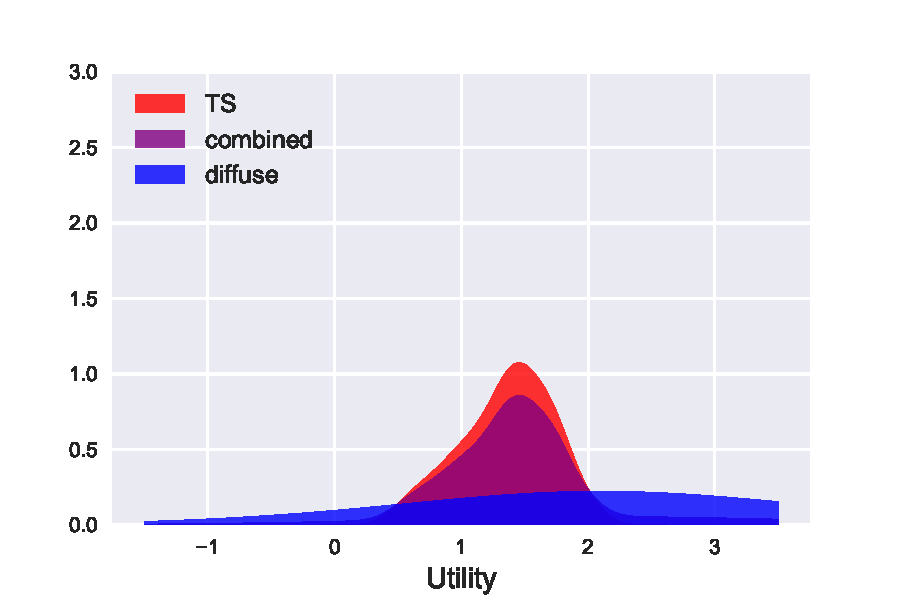
\includegraphics[width=.4\textwidth]{plots/utildifdis600.pdf} }}%
    \qquad
    \subfloat[Late, 1st rank]{{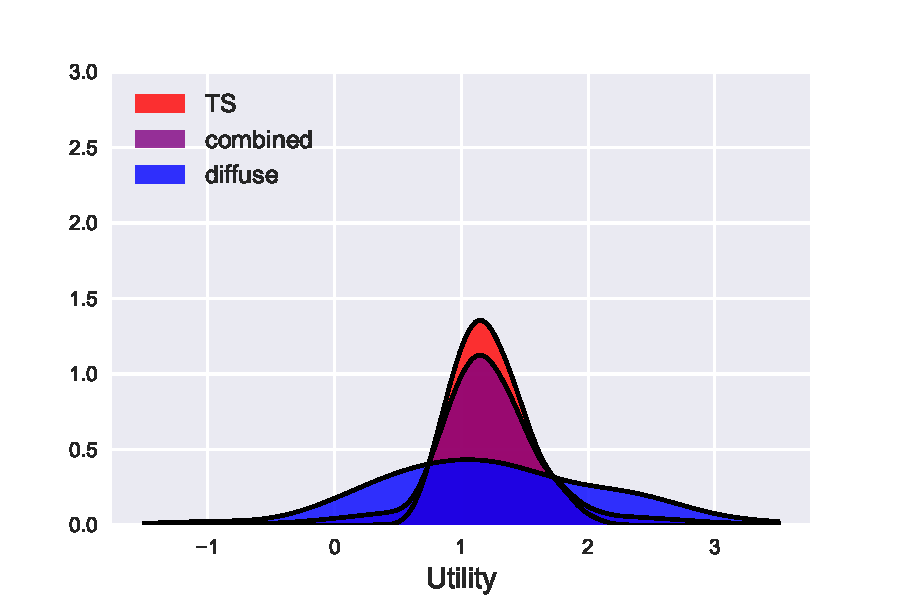
\includegraphics[width=.4\textwidth]{plots/utildifdis3000.pdf} }}%
    \qquad
    \subfloat[Early, 60th rank]{{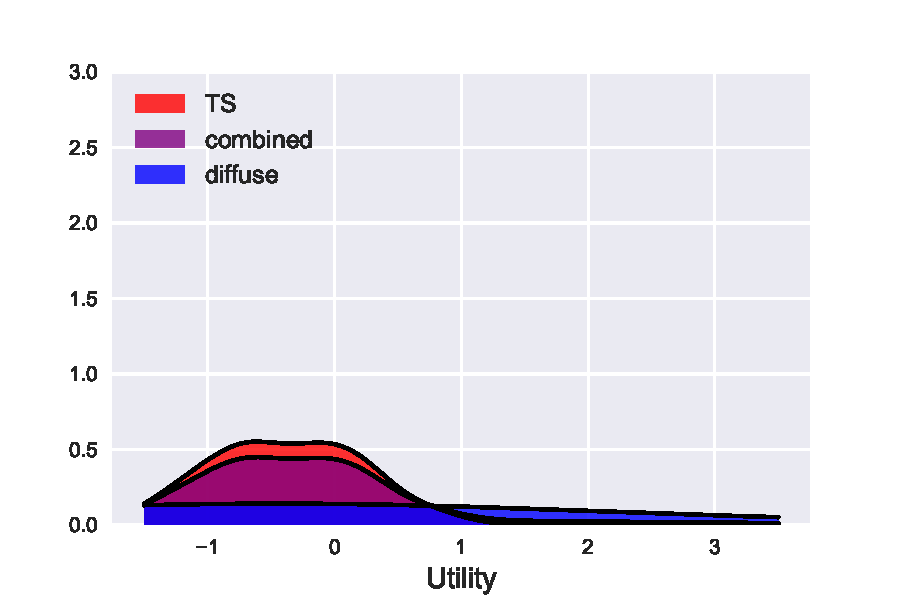
\includegraphics[width=.4\textwidth]{plots/utildifdis6060.pdf} }}%
    \qquad
    \subfloat[Late, 60th rank]{{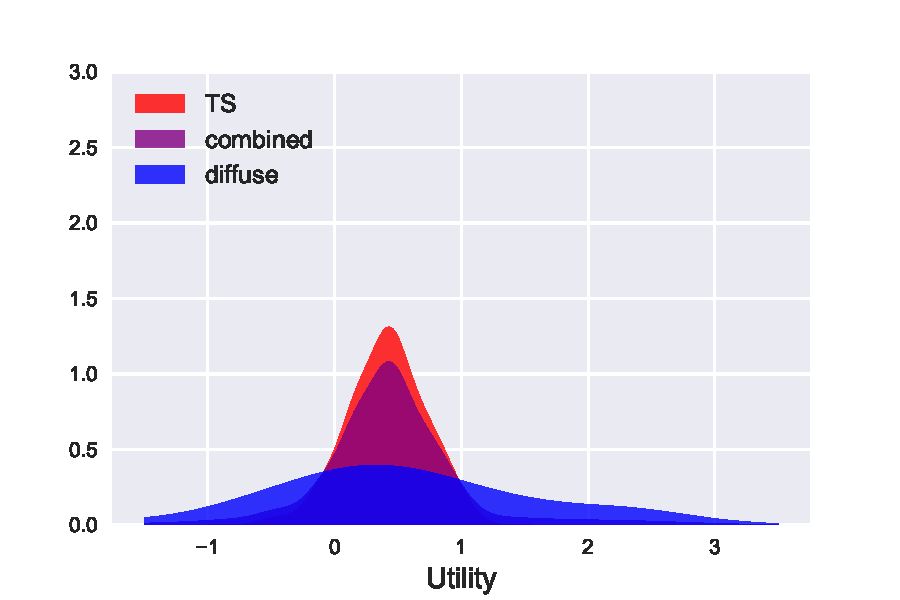
\includegraphics[width=.4\textwidth]{plots/utildifdis30060.pdf} }}%
    \end{center}
\end{figure}

For the $\epsilon$-$\delta$ case, density does not spike as quickly. Speed is controlled through two parameters: the proportion of items sampled from the diffuse distribution ($\epsilon$) and a factor increasing variance for the diffuse distribution ($\delta$). As $\epsilon$ increases and $\delta$ decreases, the algorithm slows and explores more to settle on its set of items. 

We show how \edts performance varies with different $\epsilon$ and $\delta$ values in Section \ref{sec:empirical_main}.  For our empirical analysis, we use ($\epsilon=\frac{1}{4}$, $\delta=\frac{1}{4}$). We also test ($\epsilon=\frac{1}{2}$, $\delta=\frac{1}{4}$) and ($\epsilon=1$, $\delta=\frac{1}{4}$), which perform on par with ($\epsilon=\frac{1}{4}$, $\delta=\frac{1}{4}$). Our recommended ranges for the parameters are $\frac{1}{5}\leq \epsilon \leq \frac{1}{2}$, $\frac{1}{4}\leq \delta \leq \frac{1}{2}$.

% \begin{figure}[!ht]
% \caption{Selecting your $\epsilon$-$\delta$ values. 
% 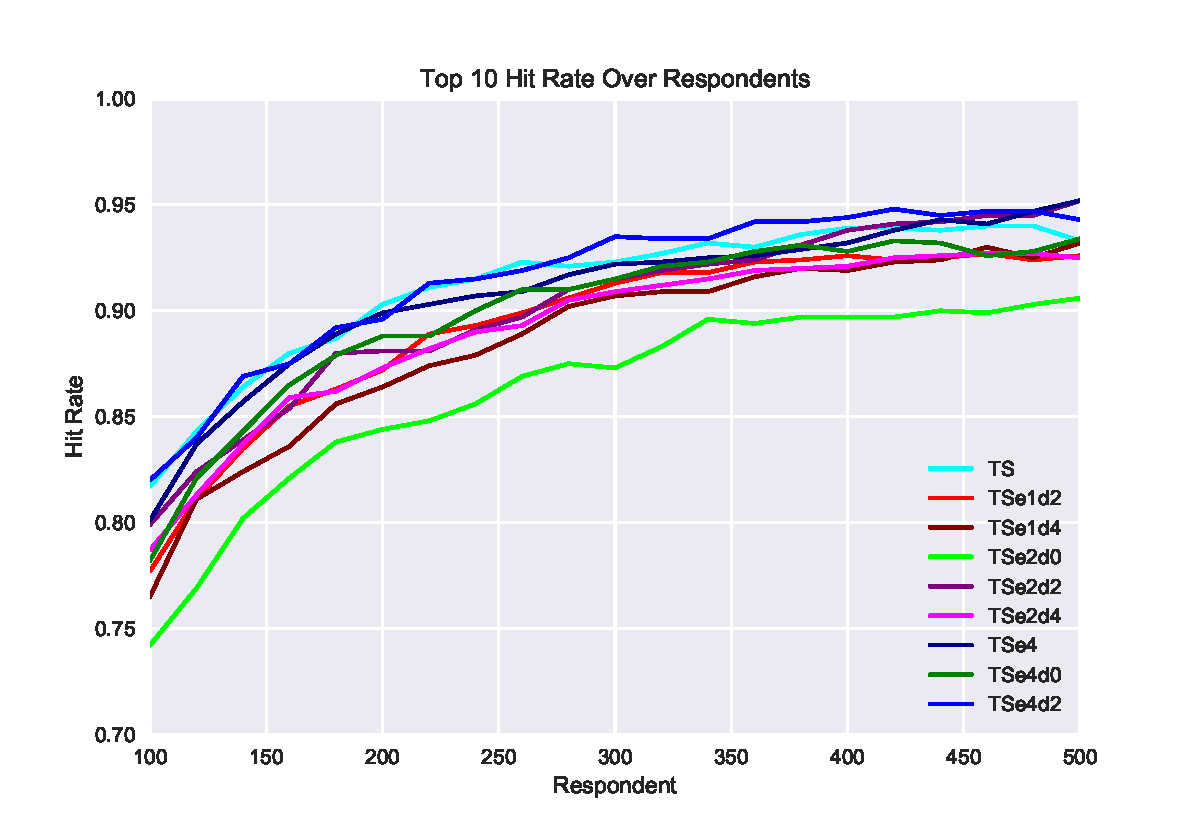
\includegraphics[width=1\textwidth]{plots/hr120v20k10ed.pdf}
% \label{fig:ed}
% \end{figure}

\subsubsection{Exploration Diffuse with Threshold}

To define an exploration-diffuse TS version with a threshold (\edtsthres), we begin with two draws: $u_R$ from the standard posterior and $u_D$ from the diffuse posterior. We calculate threshold-based item scores $s_R$ and $s_D$ for each and take $(1- \epsilon) \numperset$ items with the best $s_R$ scores and $\epsilon \numperset$ items, with the best $s_D$ scores not already included. 

As \edts nests $\epsilon$-greedy sampling, \edtsthres encompass $\epsilon$-greedy. We use the scores $s_i=|u_i - |$ for $c=\frac{u_k+u_{k+1}}{2}$ and take the $((1-\epsilon)L)$ best but sample the remaining scores uniformly (i.e., the most diffuse distribution).

\section{Preference Measurement}
\subsection{Idea Screening and MaxDiff Scaling}
\begin{figure}
\caption{MaxDiff has become more popular over time with data analysis software users} \label{fig:pop}
\begin{center}
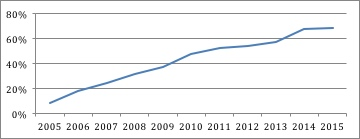
\includegraphics[width=0.5\textwidth]{plots/maxdiffpop}
\end{center}
\end{figure}
MaxDiff is a preference measurement and characteristic scaling method. In a MaxDiff questionnaire, the researcher asks respondents for their most and least preferred items out of a set and repeats the choice task for subsequent sets. Initially proposed by~\cite{louviere1991best}, MaxDiff was first released as a software system in 2004 by Sawtooth Software. Since its release, its popularity has increased steadily, and the technique was used by more than 70\% of Sawtooth Software users in 2017 (Figure \ref{fig:pop}). These users are practitioners of marketing research and consumer insights across industries.

The MaxDiff approach provides more discrimination among items and respondents than traditional rating scales \citep{cohen2004s}. It also avoids the scale-use bias common to traditional ratings techniques \citep{marley2005some,chrzan2006empirical}.

The MaxDiff technique is closely related to conjoint analysis, but MaxDiff allows the respondent to select a best and worst item instead of only one, which is what makes it best-worst scaling \citep{marley2005some}. In its most common form, MaxDiff may be thought of as a one-attribute, choice-based conjoint study with many levels. But MaxDiff can be applied to full-profile multi-attribute alternatives as well \citep{marley2012models}. The differences between conjoint and MaxDiff in their static form are not as relevant for large-scale ranking and selection problems as the differences between the adaptive versions, as the adaptive conjoint objective differs from our objective.

\subsection{Studying Many Items with MaxDiff}

Market researchers used MaxDiff for analyzing large numbers of possible consumer preferences, and the definition of ``large'' has changed in recent years. \cite{hendrix2007alternative} describe ``large sets'' as about 40 to 60 items, proposing MaxDiff variants Augmented and Tailored MaxDiff to handle them. \cite{wirth2012largeset} also investigated MaxDiff variants, Express and Sparse MaxDiff, for handling ``very large sets'' of more than 100 items. The researchers conduct a simulation study of robotic respondents using 120 items and a real study among consumer respondents with 60 items. In this paper, we refer to even larger numbers of survey items, at least 100 items and potentially 300 or more. Our goal is to explore how algorithms scale and how market researchers can push MaxDiff further than ever before.

A 2015 Sawtooth Software customer feedback survey revealed users' need to accommodate more consumer preference items (see Appendix, Figure \ref{fig:max_and_purpose}). Nearly 20\% of respondents indicated their firms had conducted a study with more than 50 items; the maximum was 400. However, according to Sawtooth Software guidance for typical problems, the recommended number of items for a MaxDiff study is about 30, and the alternative profiles recommended for a conjoint study is about 20. The respondents were also asked the main purpose for their large-scale MaxDiff studies. For 42\% of the studies, the main purpose was to identify the top or top few items. Our research shows that for such settings, traditional design strategies can be wasteful, and an adaptive approach can save firms time and money.


% One setting where practitioners consider MaxDiff studies with more than 50 or even 400 distinct product features or service characteristics is the way those items are defined. Those MaxDiff items may represent conjoined elements, like a combination of packaging style, color, claims, and highlighted ingredients. In addition, profiles involving multiple, highly interactive attributes pose challenges for choice-based conjoint analyses, making large-scale MaxDiff studies viable alternatives.


 % can be up to 4x more efficient-- without the Bandit MaxDiff approach, you are potentially wasting 75 cents of every dollar you are spending on MaxDiff data collection. 

\subsection{MaxDiff: A Best-Worst Scaling Choice Model}

In a standard MaxDiff study, every respondent selects both the best and worst option from an available set of characteristics in each discrete choice task. The model for the data comes from a class known as best-worst scaling, one of which is MaxDiff. We adopt our framework from the best-worst scaling literature \citep{marley2005some,marley2012models}. 

Suppose we a set, $S$, for each choice task. Then we can define two random variables: best ($B_z$) and worst ($W_z$) for each $z \in S$.  We then define a third random variable, best-worst $BW_{r,s}$, for any $r,s \in S$. Following a random utility framework, the utilities have deterministic and stochastic components. Thurstone provides a consistent random utility model where each $\gamma_z$ features the extreme value distribution. Because the model is consistent, we have $B_z=-W_z=U_z$ and $BW_{r,s}=U_r-U_s$ and
\begin{align*}
&B_z=v_z+\gamma_z\\
&W_z=-v_z-\gamma_z\\
&BW_{r,s}=v_r-v_s+\gamma_r-\gamma_s.
\end{align*}We can write the probability an item is the best and worst as
\begin{align*}
&B_S (x)= Pr⁡( B_x=\max_{z \in S} B_z)\\
&W_S (y)= Pr⁡( W_y=\max_{z \in S} W_z).
\end{align*}
Without using the particular utility or item scale, we can derive choice probabilities. In the most general form, we suppose $b()$ and $w()$ are separate interval scales. The resulting probability of an item being best or worst is
\begin{align*}
&B_S (x)= \frac{b(x)}{\sum_{z \in S}b(z)}\\
&W_S (y)= \frac{w(y)}{\sum_{z \in S}w(z)}.
\end{align*}
For any pair of items $x,y \in S$, we can indicate the joint probability that $x$ is best and $y$ is worst. However, when considering best and worst together, the scales $b$ and $w$ are not separately identified. We fix their ratio for the same item by setting $w(z)=\frac{c}{b(z)}$. The resulting joint probability is a function of the scale ratios for pairs: 
\begin{align*}
&BW_S(x,y)=Pr(U_x>U_z>U_y | z \in S -\{x,y\}, x\neq y)\\
&BW_S(x,y)=\frac{b(x)/b(y)}{\sum_{r,s \in S, r \neq s}b(r)/b(s)}.
\end{align*}
To accommodate the standard utility structure, we let utility $u(z)=\log{(b(z))}$, making each of the probabilities 
\begin{align*}
&B_S(x)=\frac{e^{u(x)}}{\sum_{z \in S} e^{u(z)}}\\
&W_S(y)=\frac{e^{u(y)}}{\sum_{z \in S} e^{u(z)}}\\
&WB_S(x,y)=\frac{e^{u(x)-u(y)}}{\sum_{r,s \in S, r\neq s} e^{u(r)-u(s)}}.
\end{align*}
We can derive the same representation from the random utility model suggested by \cite{marley2005some}. We can view best-worst choice as a generalization of the classic multinomial logit technique for selecting best only.

\subsubsection{Best-Worst Model Estimation}

One way to estimate the MaxDiff choice model is to enumerate all possible pairs of items and describe the joint probability of being best and worst. This is the probability of yielding the largest difference $BW_S(x,y)$ in consumer behavior. This pairwise approach is not practical because it scales quadratically for number of items. So, we adopt an alternative approach reflecting the literature and practice that is shown to be a near exact approximation of the full model \cite{cohen2003maximum}. This allows us to estimate the best model and worst model independently, without explicitly estimating the best-worst probability. (See Appendix for details.)

%\textbf{Emphasize our goal is to identify the top items.}

\section{Bandit MaxDiff}

%We utilize the best available bandit alogrithms and draw upon the active learning and best k arm identification problems. Thompson Sampling involves allocating resources to an action in proportion to the probability that it is the best action~\cite{thompson1933likelihood}. 

Our proposed approach, Bandit MaxDiff, incorporates adaptive learning as a natural method for solving top-set ranking and selection problems. Our approach leverages prior learning during survey administration to create more efficient questionnaires and more precise aggregate score estimates. On the one hand, we want to come to a conclusion about the relative importance of a large number of product or service characteristics within a MaxDiff problem. On the other hand, we want to utilize what we have learned as we go to target actions likely to allow the researcher greater precision. TS has proven useful for these types of problems \citep{schwartzetal2017,russo2017tutorial}.

For each of our survey respondents, we select $\numperset$ items and generate a MaxDiff design of $J$ best-worst tasks, each with a choice set of $|S|$ items. For example, as our empirical default, we use $\numperset=20$, $J=12$, and $|S|=5$, standard numbers used in MaxDiff studies \citep{wirth2012largeset}. 

We begin as in a traditional MaxDiff design, showing each item an equal number of times across all respondents and tasks to ensure a balanced design.  For the first respondent, we select the $\numperset$ items uniformly. 

After the initial respondent batch, we remain uncertain about each item's parameter value, so we continue collecting data. But we do not need to reduce uncertainty equally, so we adapt strategically. At each subsequent period after collecting a set amount of respondent data, we estimate a model to characterize our parameter beliefs. We systematically oversample the items already viewed as most preferred, the top set. But we also recognize our uncertainty about the top-set items. Figure \ref{fig:dots} shows the oversampling as data accumulate. As the sample size increases, uncertainty around which items are best tightens.

\begin{figure}[!ht]
\caption{Respondent-by-item counts are shown to illustrate oversampling as data accumulate.}
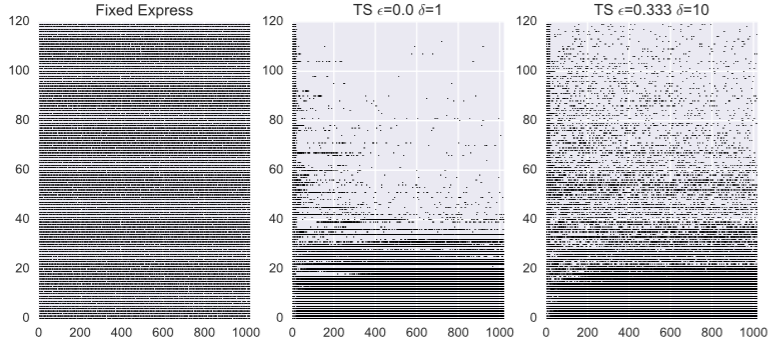
\includegraphics[width=1\textwidth]{plots/3dotplot-lowres.png}
\label{fig:dots}
\end{figure}

Bandit MaxDiff uniquely translates our current beliefs about parameters into decisions about what to ask subsequent respondents via oversampling the best items in a principled manner. The approach is summarized in Table \ref{methods}.

\begin{algorithm}
\caption{Bandit MaxDiff: \ts} \label{alg:ts_simple}
\begin{algorithmic}[1]
\State Given: $K,\numperset,J,S,b$.
\State Initialize first set of questions by sampling $\numperset$ items uniformly.
\State Design MaxDiff questionnaire covering $\numperset$ items with $J$ tasks of $S$ questions each, $\text{MDDesign}($\numperset$,S,J)$, for the next batch of $b$ respondents.
\State Collect new data from respondents with $n = b*t$ respondents.
\State Bayesian Bootstrap sample weight replacement using weights ($\alpha_1, ...., \alpha_n)\sim \text{expon}(1)$, obtaining some subset of $n$ previous respondents.
\State Estimate model parameters ($\theta_t$) and obtain estimated utilities $u = (u_1,...,u_K)$.
\State Choose $\numperset$ items using draws from empirical posterior.
\State Select next questions for respondents.
\end{algorithmic}
\end{algorithm}

% $S=\#\{\mathcal{S}\}$

\subsection{Bandit MaxDiff and Posterior Sampling} \label{sec:bmd_ts_edts}

The Bandit MaxDiff base algorithm draws on TS to address the multi-armed bandit problem. The method's specific instantiation is shown in Algorithm \ref{alg:ts_simple}.
  
\subsubsection{Learning with Bayesian Bootstrapping}

For TS models, we first characterize parameter uncertainty. We use a multinomial logit model; the first but least practical option to obtain posterior draws would be to use the Markov Chain Monte Carlo, which would be too slow to update in real time. A more practical way to approximate the posterior is to sample from the asymptotic distribution via the maximum likelihood implied by the estimated mean and standard errors, a Laplace Approximation of the Posterior \citep{tierney1986accurate}. The Laplace approach reflects the estimated population preferences and normally distributed error, with standard deviations equal to the standard errors of the parameter estimates. The method would work quickly, but it forces the joint posterior into a multivariate normal distribution. 

We can obtain posterior samples using the Bayesian Bootstrap method by sampling weights $\beta$ for each respondent: $\beta_1,\beta_2,\ldots,\beta_N \sim \text{exp}(1)$. The weights are used for sampling respondents with replacements to form a new bootstrapped dataset. If a respondent is sampled, all the data is included in the bootstrapped sample. The probability of any one respondent $i$'s data being sampled in any one draw is $\beta_i / \sum_{i}^{N}\beta_i$.  For each bootstrapped dataset, we obtain parameter estimates of $\theta$ using a weighted  maximum likelihood estimate as follows:
\begin{align}
&LL(\theta;\beta)=\sum_{n=1}^N \beta_n
\sum_{x \in S_n} 
	\left(
		Y_{B_{S_n}}(x)
		\log{\frac{e^{\theta_x}}{\sum_{z\in S_n} e^{\theta_z}}} 
		+ 
		Y_{W_{S_n}}(x)
		\log{\frac{e^{-\theta_x}}{\sum_{z\in S_n} e^{-\theta_z}}}
	\right) \\
&\theta^\beta = \text{arg}\max_{\theta} LL(\theta;\beta) ,
\end{align}

where each estimate $\theta^\beta = u_1^\beta, \ldots, u_K^\beta$ implies a rank ordering of all items $\pi_{u}^{\theta^\beta} = \pi(1),\ldots,\pi(\numperset),\pi(\numperset+1),\ldots,\pi(K)$. The items corresponding to $\pi(1),\ldots,\pi(\numperset)$ form the next list of $\numperset$ items to show the next respondent. 

While the Bayesian Bootstrap is rarely used for posterior sampling, we use it throughout our empirical application because of its conceptual appeal and speed. Because we only need one set of $\numperset$ items per respondent, we can obtain new bootstrapped samples $\theta^{\beta}$ and $\pi(u|\theta^\beta)$ for each new respondent. If we seek the probabilities with which any item would be selected, we can obtain many independent and parallelized samples. 

\subsubsection{Bandit MaxDiff and \ts Intuition }

While collecting data for the Bandit MaxDiff algorithm, imagine we have 100 respondents and can summarize the population's preferences for 300 characteristics, with their item-specific parameter values in a multinomial logit model. To generate a MaxDiff task for the 101st respondent, we draw from the population preferences, leveraging mean estimates and normal errors with standard deviations equal to the standard errors' point estimates. We sort the newly sampled vector of preference values from the most to least preferred item. The most preferred can be used to create the sequence of MaxDiff choice tasks for the 101st respondent.

A typical bandit algorithm is not practical here. While selecting an arm means including an item in the survey for the next respondent, the reward is not revealed each period. Since each respondent must see only a subset of items, the item receiving the ``best'' label in a choice task does not translate directly to a reward. The choice data allows us to infer how each item ranks among all characteristics, aligning with our managerial goal.

The posterior variation---the sample-to-sample differences in parameter value and relative rank ordering---is critical. Even when little data has been collected, we have substantial uncertainty. The independent samples differ in rank order of item utilities. This allows MaxDiff designs across respondents with less overlap in items. Later, uncertainty is reduced most around the truly high-utility items. Across independent samples, item ranking is highly correlated near the top but not near the bottom, where uncertainty remains. As a result, the top subset of $\numperset$ items selected converges to the same group for each respondent. The algorithm learns over time, identifying items with truly high utility with high precision (Figure \ref{fig:illustrate_ts}). 

\begin{figure}
\caption{Shown is an illustration of a MaxDiff Thompson Sampling procedure.}
\label{fig:illustrate_ts}
	\begin{center}
    \subfloat[Early]{{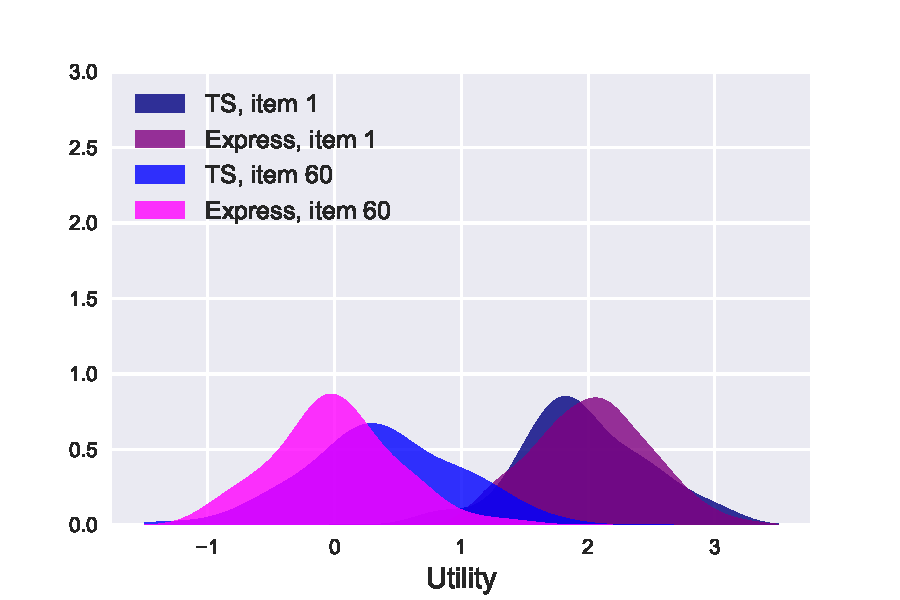
\includegraphics[width=.4\textwidth]{plots/utildis60.pdf} }}%
    \qquad
    \subfloat[Late]{{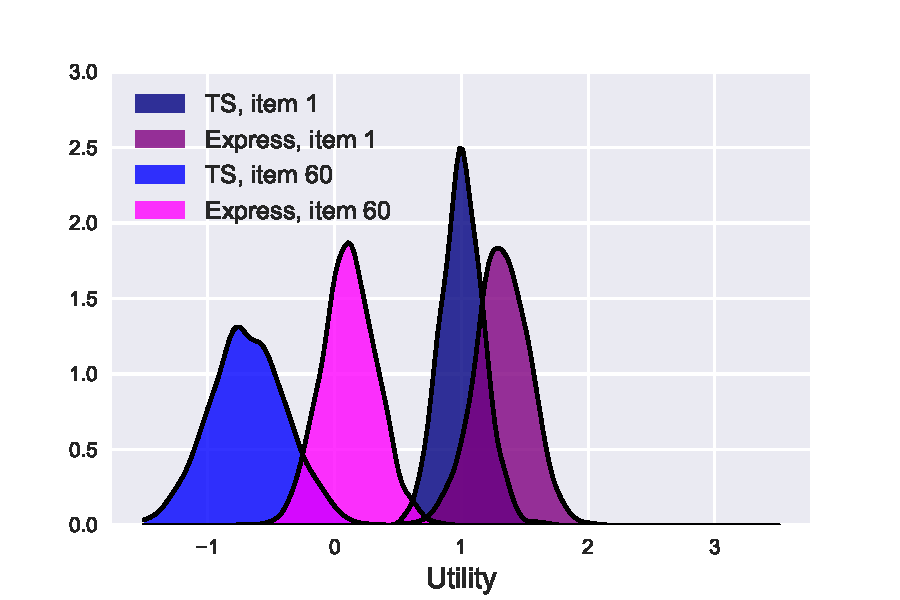
\includegraphics[width=.4\textwidth]{plots/utildis300.pdf} }}%
    \end{center}
\end{figure}

\subsection{Exploration-diffuse Thompson Sampling}

Changes over time can cause robustness issues for TS algorithms. On the one hand, TS features built-in robustness---the algorithm is stochastic and adapts continuously. If early survey data leads the algorithm astray, it will self-correct, eventually finding and converging on the respondents' most preferred items. 

Suppose  early respondents make choices leading the researchers to believe certain survey items are best when they are not. Subsequent respondents will then be shown the items, and uncertainty will be reduced, indicating other items are likely better. By sampling from the item utilities' joint belief distribution, we will be less likely to draw the items which will eventually be shown as poor performers. 

Such sampling could be too aggressive, as the natural parameter uncertainty is not sufficient. Or it may be too slow to adjust to large changes in the sampled respondents, reflecting either a shift in the population or that the earlier respondents are not representative of the broader population. This potential problem can be addressed with \edts.


\begin{table}
\begin{tabular}{p{3in}|p{3in}}
Algorithm & Description of sampling scheme \\
\hline
MaxDiff TS & Take $\numperset$ items with highest utility sampled from the posterior.\\
MaxDiff $\epsilon$-Diffuse TS & Take $(1-\epsilon)L$ items with highest utility sampled from the regular posterior; sample from diffuse posterior distribution, and take $\epsilon L$ items with highest sampled utility from remaining items.\\
$\epsilon$-Greedy & Take $(1-\epsilon)L$ with greatest current estimated $\theta$; take remaining $\epsilon L$ uniformly from remaining items.\\
TS Closest to the Threshold & Take $\numperset$ items with sampled utility closest to $\frac{u_k+u_{k+1}}{2}$.\\
$\epsilon$-Diffuse TS Closest to the Threshold & Take $(1-\epsilon)L$ (from posterior) and  $\epsilon L$ (from diffuse posterior) items with sampled utility closest to $\frac{u_k+u_{k+1}}{2}$.\\
$\epsilon$-Greedy Closest to the Threshold & Take $(1-\epsilon)L$ items with estimated utility closest to $\frac{\theta_k+\theta_{k+1}}{2}$ and $\epsilon L$ items uniformly from remaining.\\
Misclassification Minimization with Random Perturbation& Take $\numperset$ items most likely misclassified (bottom items that should be top and vice-versa); add perturbation to probability.\\
Greatest Uncertainty with Random Perturbation& Take $\numperset$ items with probabilities of being top at closest to 50\%; add perturbation to probability.\\
\end{tabular}
\caption{Summary of Adaptive MaxDiff Algorithms.}\label{methods}
\end{table}

% \textbf{Shea: Make captions for all tables flush left}

%%Discuss relation to the Follow the regularized leader / perturbed leader 

% \subsection{BAM for Best-Arm Identification}

% \subsubsection{New Variant: Closest to the Threshold}

% \begin{verbatim}
%        utilities        rank ordering
% item : a b c d e f   max(1)(2)(3)(4)(5)(6)min
% draw1: 6 7 7 8 8 9  -->  f  d  e  c  b  a   
% draw2: 7 5 5 9 8 6  -->  d  e  a  f  b  c 
% draw3: 6 4 5 8 7 5  -->  d  e  a  c  f  b 
% \end{verbatim}

% \subsubsection{Algorithm Misclassification Minimization}

\subsubsection{Fixed Express MaxDiff}
We uniformly and randomly draw $\numperset$ of $K$ items without replacement to show to each respondent, achieving balance across items and respondents. For example, in a problem with $\numperset=20$ of $K=120$, each item appears $\frac{J*S}{L} = \frac{12*5}{20} = 3$ times per respondent on average.

\subsubsection{$\epsilon$-Greedy}
We test $\epsilon$-greedy as a baseline for our adaptive methods, letting $\theta$ be the current estimated parameters. We take the $(1-\epsilon)L$ items with the greatest $\theta$ value and choose the remaining $\epsilon L$ uniformly. We use $\epsilon=\frac{1}{4}$ for our empirical analysis and test others. For greedy alone, $\epsilon=0$ would always serve the top $\numperset$ items with the highest estimated average utility to subsequent survey respondents.

\section{Empirical Analysis: Main Results}

\label{sec:empirical_main}
We compare our proposed set of adaptive approaches to existing adaptive and non-adaptive strategies. We use simulated choice data based on inferred preferences from an actual MaxDiff survey.

\subsection{Data}
Our data, which include 981 respondents and 120 items, come from a survey conducted by P\&G using Sawtooth Software. The items represent product features and benefits, but the subject matter and item text is hidden for confidentiality purposes. The questions come from a sparse MaxDiff study using a fixed, non-adaptive design with balance across all items and respondents. 

Instead of raw choice data, P\&G provides the individual-level posterior mean utilities for all respondents and items, which are obtained via Markov Chain Monte Carlo sampling for a hierarchical Bayes (HB) logit model. We call the individual-level utilities the true HB utilities. The utilities offer realistic preference patterns across the items and respondents and generate data for our respondent simulations.  Therefore, our simulated respondents mimic the actual respondents' preferences on average---to answer each new MaxDiff task, we perturb the true HB utilities by independent and identically distributed Gumbel error.

\subsection{Simulation Setup}
To measure performance, we consider a range of metrics: item utilities' estimated rank order, correct hit rate for estimated top-ranked item sets, estimated top set utility values, and variability around estimated utilities. We obtain the measures by comparing estimates to true values. For each respondent batch, we run aggregate logits and compare the estimated utilities' current rank order to the true rank order for the known utilities, represented by aggregate averages across all respondents' true individual-level utilities. We run the simulations 100 independent times to obtain a distribution of measures. 

Our primary performance measure is \textbf{top $k$ hit rate}, or the percentage of true top $k$ items that appear in the estimated top $k$ set. For example, if the estimated scores identify seven of the true top-10 items, irrespective of order, the hit rate is 70\%. We use $k=3,10,20,40$. 

Hit rate is a natural consideration in an active learning problem. It evaluates the quality of the adaptive learning procedures with respect to the eventual decision. Hit rate is also related to regret in solving typical multi-armed bandit problems. It reflects how far we are from always selecting the truly best set of arms for all time periods. But our problem is not equivalent to the standard bandit setting, as we do not have an observed reward like clicks or purchases. 

\begin{figure}[!ht]
\caption{The plot shows the rank order and utility values on the logit scale for all 120 items in the survey, highlighting the top 10 (blue) and top three (red) items. The values become the means for the unobserved data-generating process.}
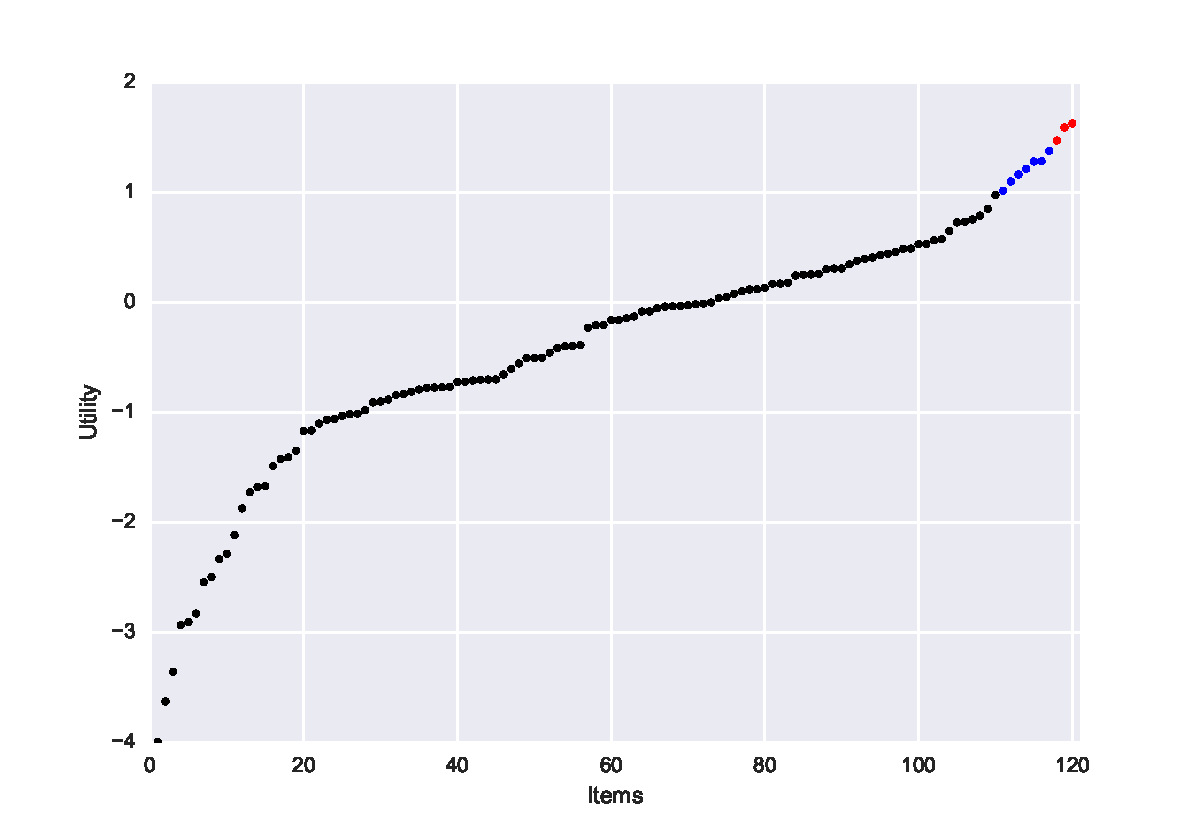
\includegraphics[width=1\textwidth]{plots/utilscore.pdf}
\label{fig:util} 
\end{figure}

The differences among the top-item utilities makes identifying the truly best items difficult (Figure \ref{fig:util}). With 120 items in the dataset, we observe that the true preferences for approximately the top 15 respondents are within 1.0 on a logit scale in terms of utility. Due to how tightly the top items are clustered, the hit rate measures we employ are highly discriminating between competing methods.

In the base setting, we simulate the process of collecting survey data from $N=500$ respondents in batches of $b=20$ per period, using bootstrap sampling with replacement from the original 981 individuals. We consider the first 20 respondents the initial group, which always receive $\numperset=20$ items uniformly selected for all methods. All adaptive methods begin after the 20th respondent. Each simulated respondent completes $J=12$ choice sets (best-worst tasks), where each set includes $S=5$ items.

We test the different adaptive approaches found in Table \ref{methods}. For our base setting, we use ($\epsilon=\frac{1}{4}$, $\delta=\frac{1}{4}$) for $\epsilon-\delta$TS methods. The natural benchmark is the existing fixed MaxDiff approach.

\subsection{Results: Greedy, Thompson Sampling, $\epsilon-\delta$ TS, and Fixed Express}

Our initial results show even simple adaptive methods perform better for large scale ranking and selection problems than static approaches. But a simple adaptive greedy algorithm, which does not explicitly incorporate learning, does not perform well enough. Table \ref{fig:simple_result} shows how TS improves substantially over the greedy approach, and \edts shows even more improvement for hit rate.

\begin{figure}
\caption{The plots show results for the \fixedexpress, \egreedy, \ts, and \edts algorithms for k=3, K=120, and L=20. Performance represents cumulative hit rate per number of respondents at that point in time.}
\label{fig:simple_result}
\begin{center}
	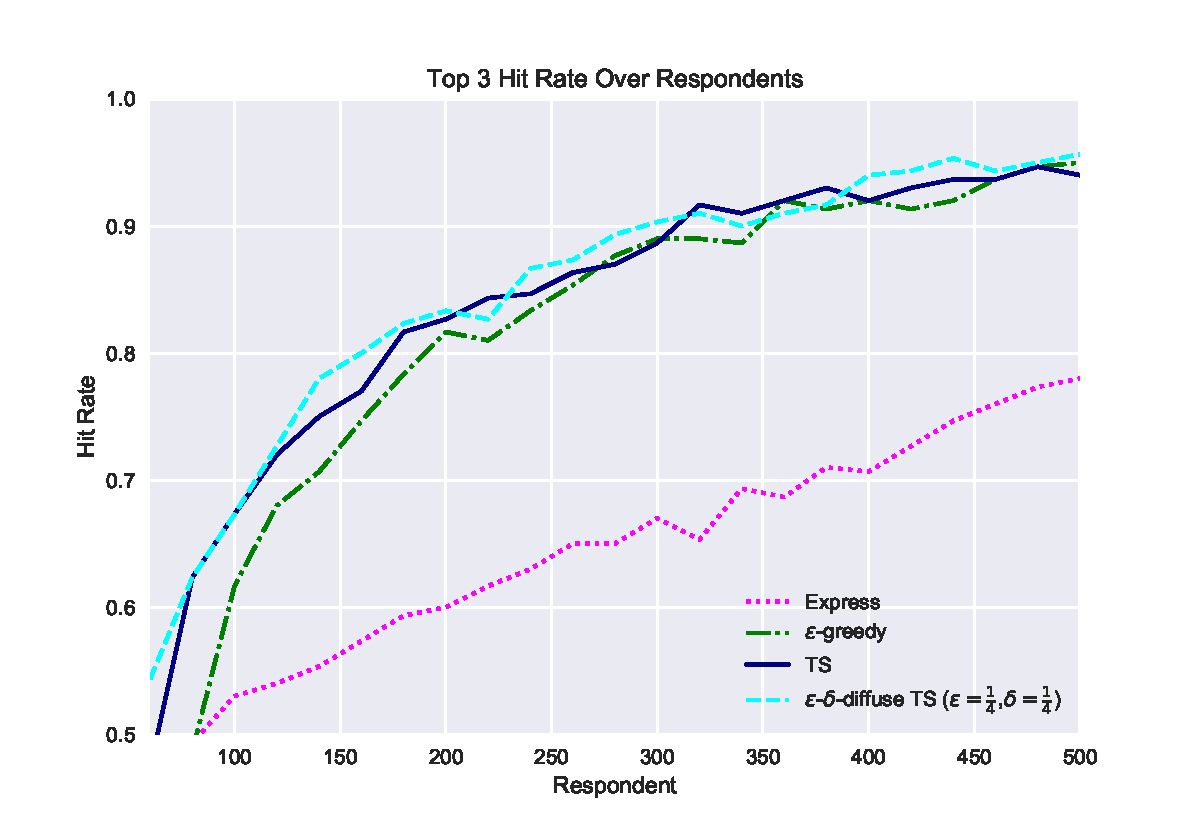
\includegraphics[width=.8\textwidth]{plots/hr120v20k3.pdf}
\end{center}
\end{figure}

After the first 200 respondents, the Fixed Express design obtains a top-three hit rate of 60\%, where the TS-based approaches achieves a top-three hit rate of about 80\%. Practically, if a marketing researcher wants a hit rate of 80\%, the methods can achieve it with a smaller sample size. But the high performing adaptive methods are at least three times more efficient than the standard Fixed Express MaxDiff approach. This holds for the different values tested in the basic setting. 

Figure \ref{fig:effects_epsilon_delta} shows how $\epsilon$ and $\delta$ affect performance. 

\begin{figure}
\caption{The plots show performance with $\epsilon = 1/2$ (left) and $\epsilon = 1/4$ (right), with multiple lines in each plot: $\delta = 1/2$ (dash-dot) and $\delta = 1/4$ (dash). Each of the plots show standard \ts ($\epsilon = 0$, $\delta =1$) performance.}
% Need to remove \delta = 0 from plots.
\label{fig:effects_epsilon_delta}
 	\begin{center}
    \subfloat[$\epsilon=1/2$]{{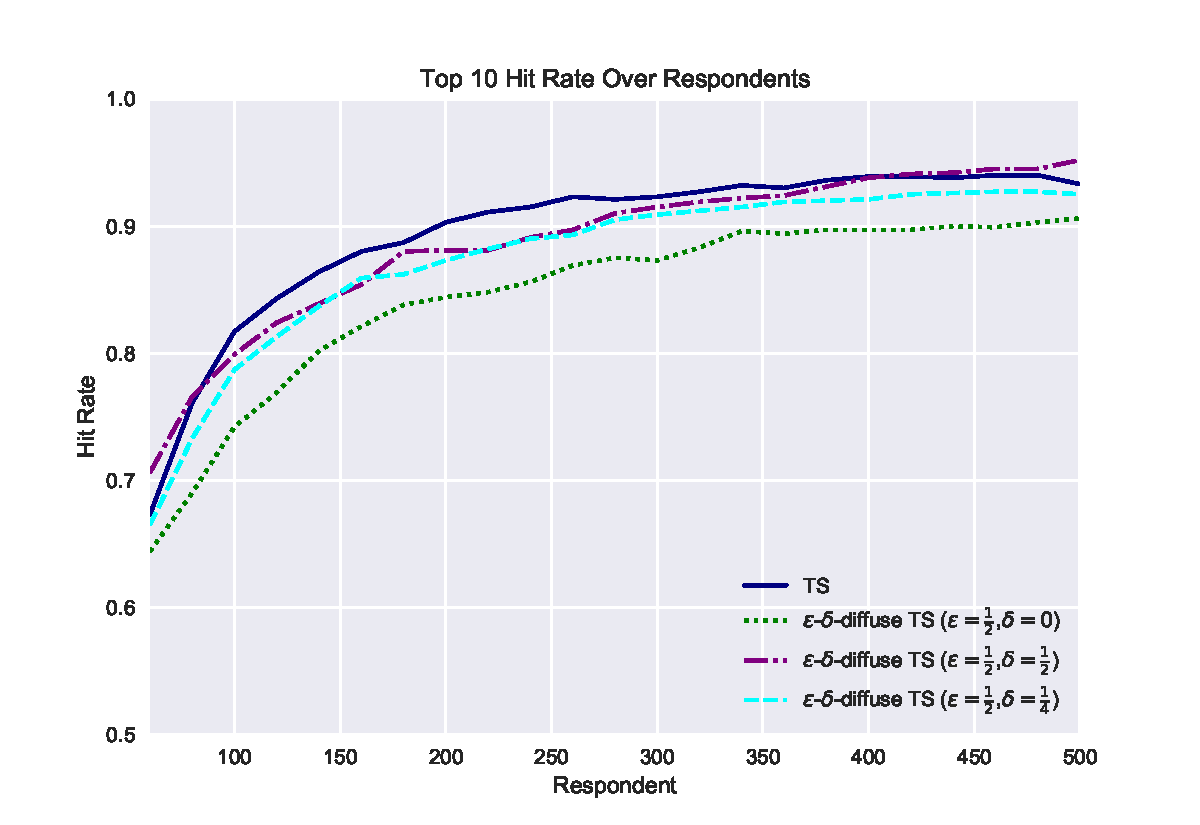
\includegraphics[width=.4\textwidth]{plots/hr120v20k10e2.pdf} }}%
    \qquad
    \subfloat[$\epsilon=1/4$]{{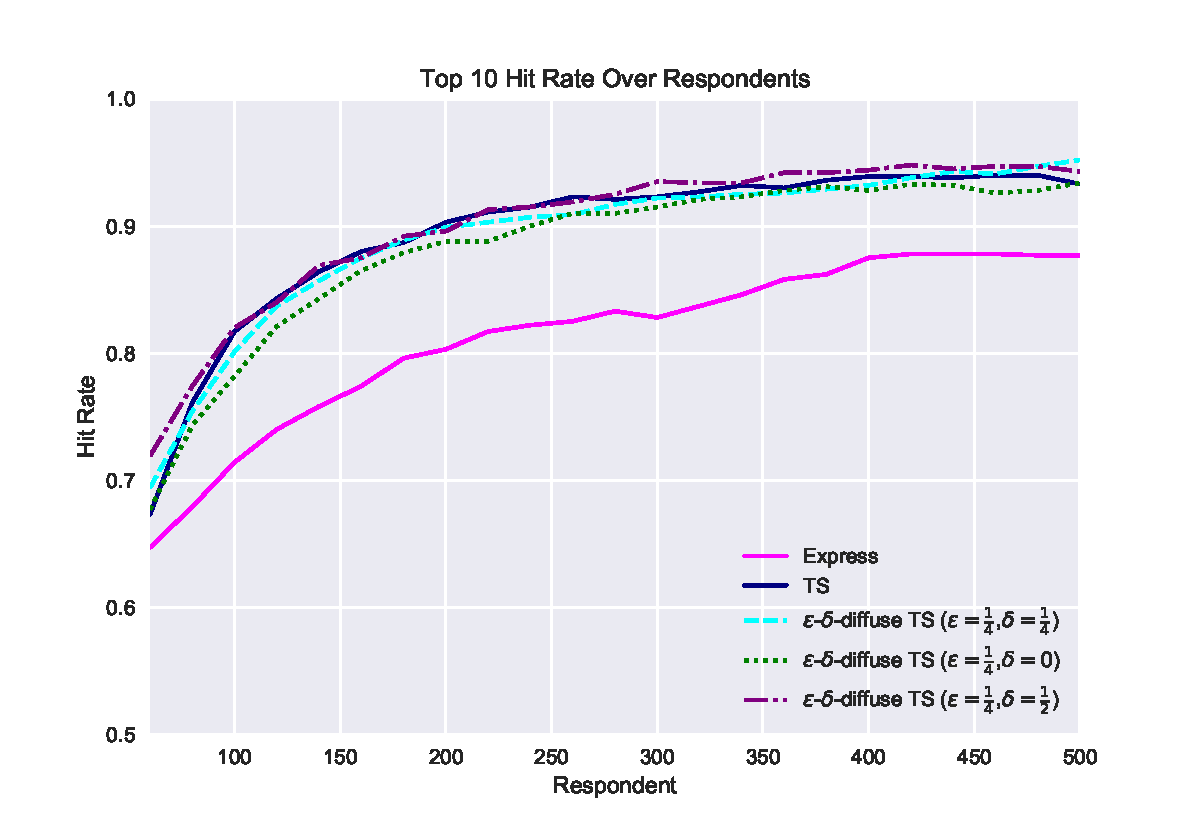
\includegraphics[width=.4\textwidth]{plots/hr120v20k10e4.pdf} }}%
    \end{center}
\end{figure}

The performance gap between TS and \edts widens dramatically when considering non-stationary settings, such as a misinformed start (see Section \ref{sec:robust}). 

\subsection{Results: Thresholding, Uncertainty Reduction, Misclassification}

Each algorithm selects $\numperset=20$ items to show every respondent. We examine hit rate for the top $k$ items, $k = \{3,10,20,40\}$. Smaller $k$ values make the problem more challenging early in the process, as selecting the top three out of 120 is more difficult than selecting the top 40 out of 120, particularly in light of the true utility value distribution (Figure \ref{fig:util}).  


Figure \ref{fig:K120_L20_k3hit_k10hit} and Table \ref{table:at_260_500} show the results for the $K=120$-item dataset serving $\numperset=20$ questions per respondent, where all methods are tested.


\begin{figure}%
    \caption{For top $k=\{10,20\}$ with 120 items, the cumulative hit rate obtained (y-axis) improves with the number of respondents interviewed (x-axis) at different rates for each algorithm.}%
    \label{fig:K120_L20_k3hit_k10hit}%
 	\begin{center}
    \subfloat[Top 10]{{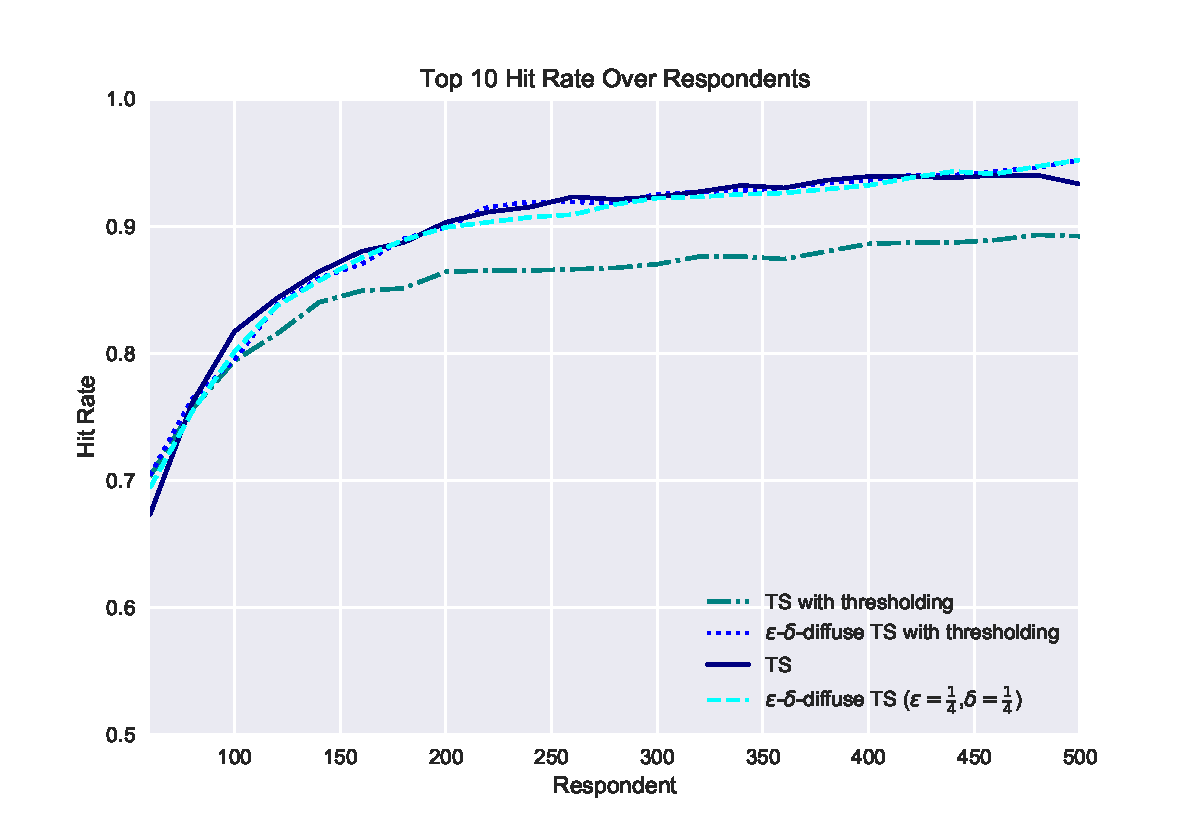
\includegraphics[width=.8\textwidth]{plots/hr120v20k10thres.pdf} }}%
    \qquad
    \subfloat[Top 20]{{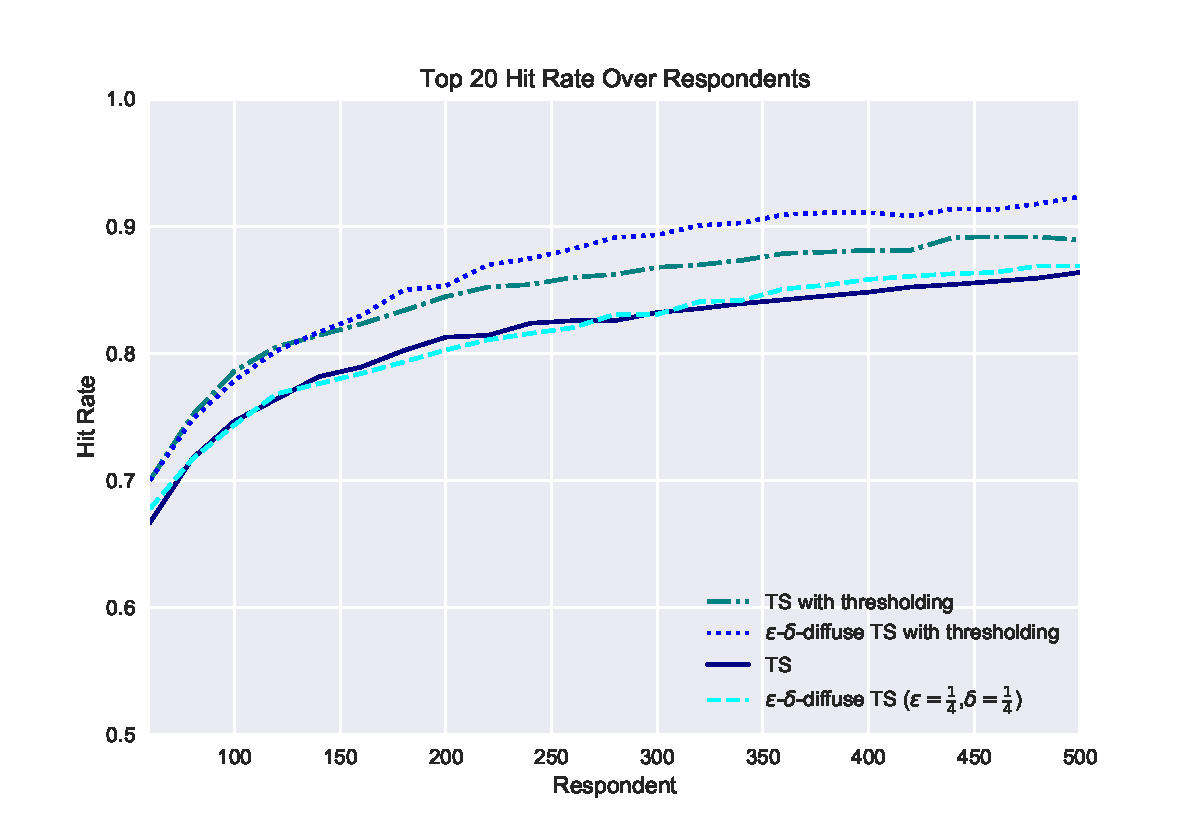
\includegraphics[width=.8\textwidth]{plots/hr120v20k20thres.pdf} }}%
	\end{center}
\end{figure}
%\eric{Why is \ts better than \tsthres for $k=10$?  Explain why in a good way \tsthres always does worse than \edtsthres. }

\begin{figure}%
    \caption{For top $k=20$ with 120 items and 20 items per person, the cumulative hit rate obtained (y-axis) improves with the number of respondents interviewed (x-axis) at different rates for each algorithm. }%
    \label{fig:K120_L20_k3hit_k10hit}%
 	\begin{center}
    \subfloat[Top 20]{{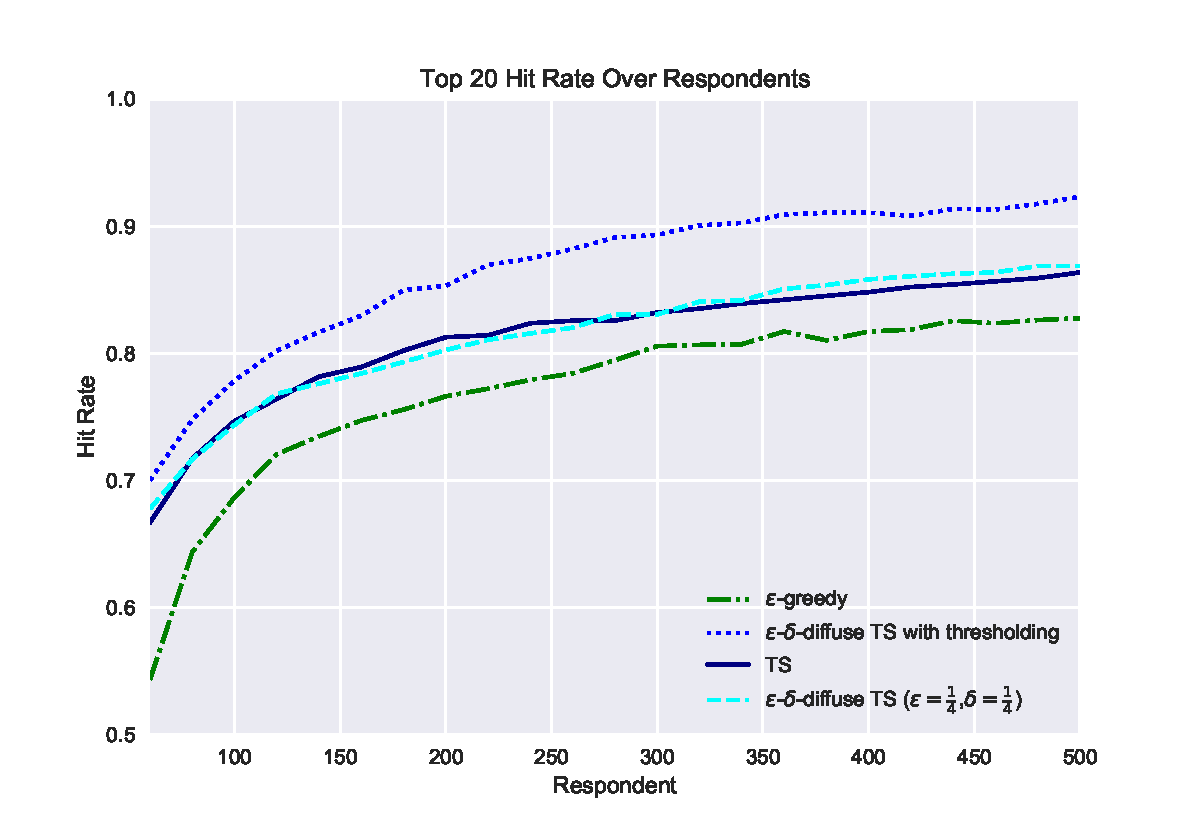
\includegraphics[width=.8\textwidth]{plots/hr120v20k20t.pdf} }}%
    \qquad
    \subfloat[Top 20]{{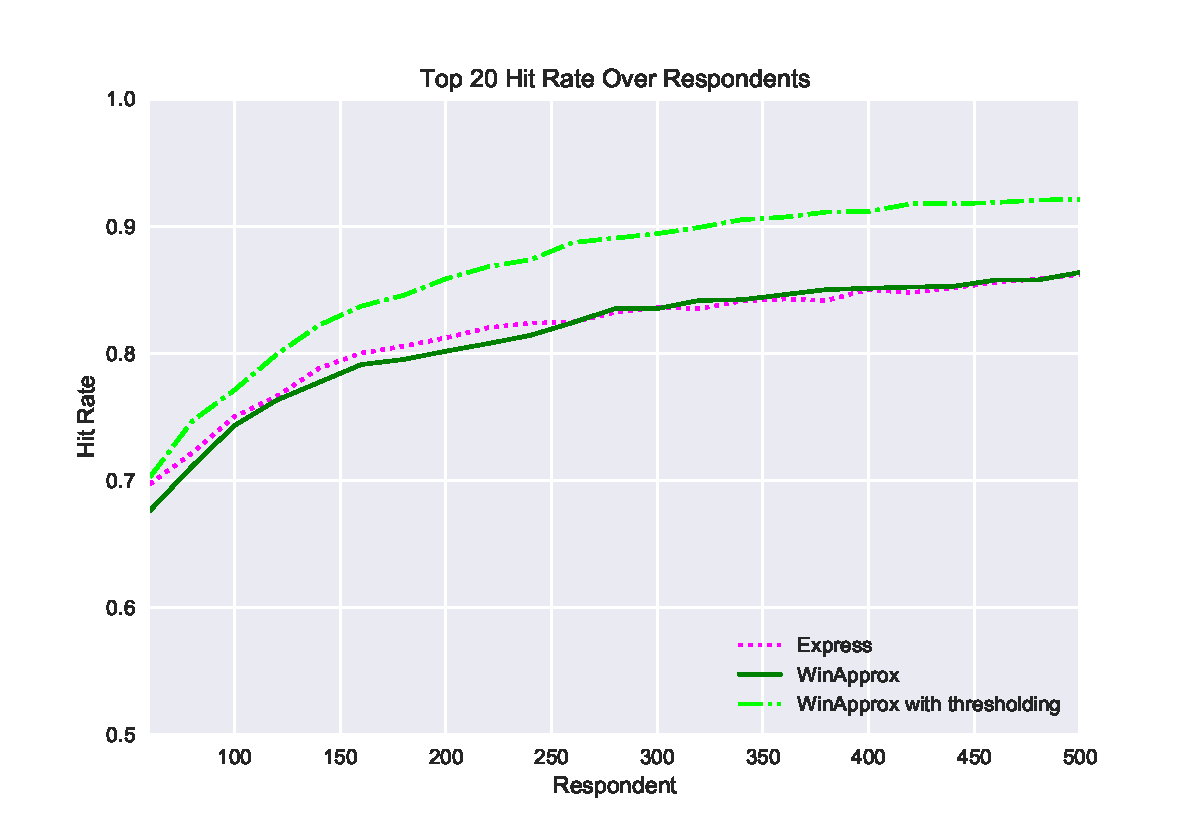
\includegraphics[width=.8\textwidth]{plots/hr120v20k20t2.pdf} }}%
	\end{center}
\end{figure}


\begin{figure}%
    \caption{For top $k=\{3,10\}$ with 120 items, the cumulative hit rate obtained (y-axis) improves with the number of respondents interviewed (x-axis) at different rates for each algorithm.}%
    \label{fig:K120_L20_k3hit_k10hit}%
 	\begin{center}
    \subfloat[Top 3]{{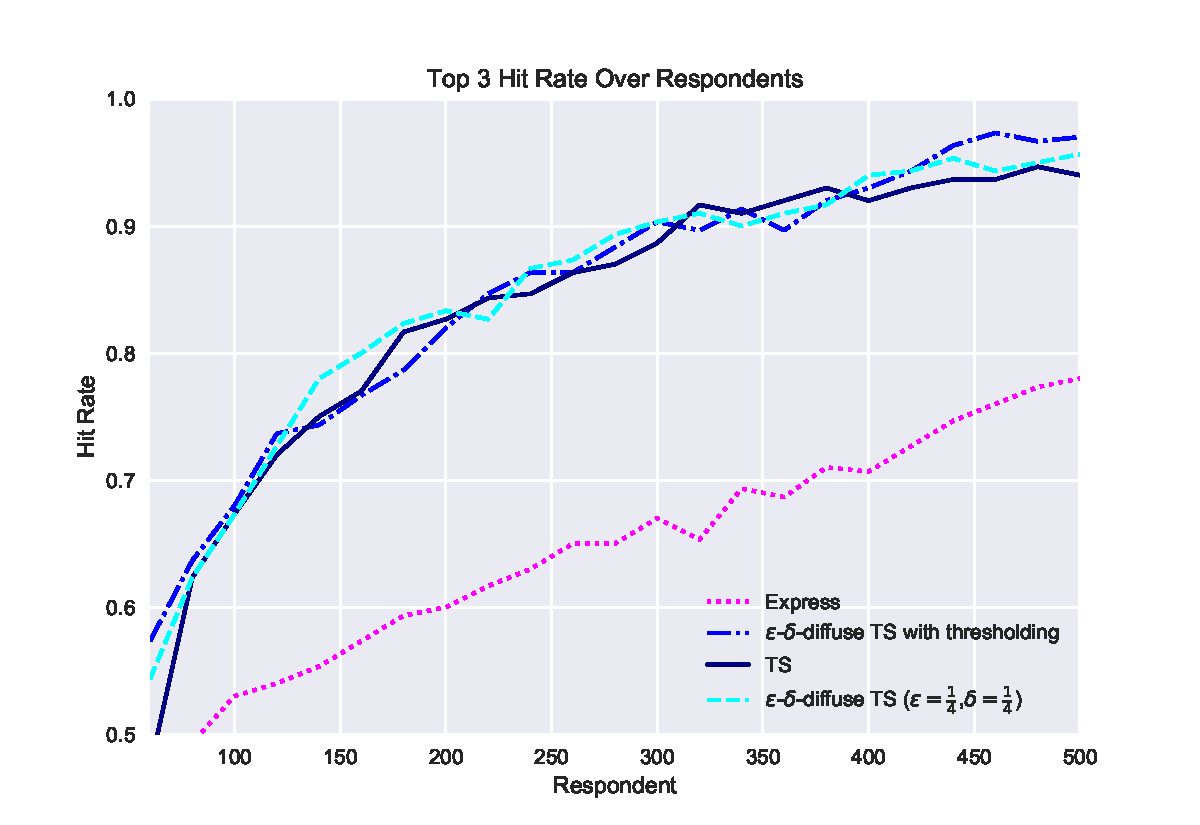
\includegraphics[width=.8\textwidth]{plots/hr120v20k3TS.pdf} }}%
    \qquad
    \subfloat[Top 10]{{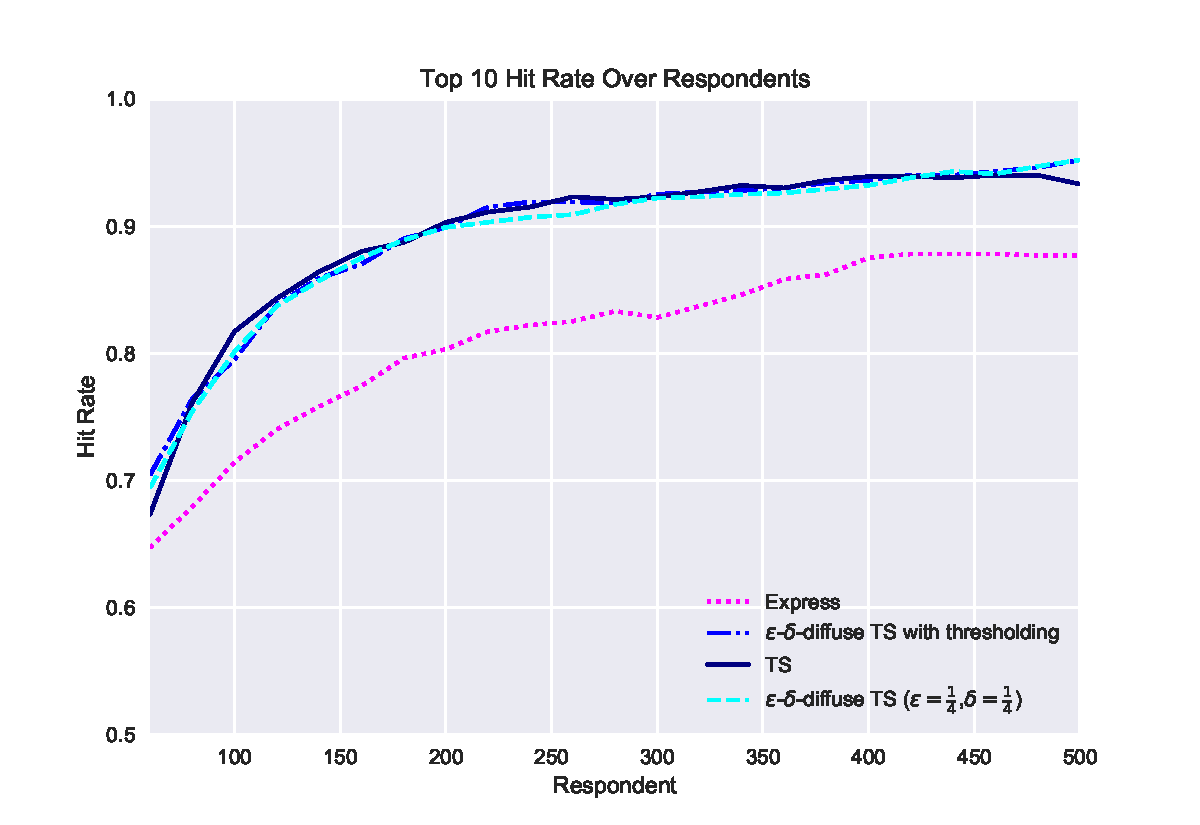
\includegraphics[width=.8\textwidth]{plots/hr120v20k10TS.pdf} }}%
	\end{center}
\end{figure}

 %\eric{Why is \ts better than \tsthres for $k=10$?   }

\begin{figure}%
    \caption{For top $k=\{3,10\}$ with 120 items, the cumulative hit rate obtained (y-axis) improves with the number of respondents interviewed (x-axis) at different rates for each algorithm. The plots show results using the \fixedexpress, \edtsthres, \mismin, and \uncert algorithms.}%
    \label{fig:K120_L20_k3hit_k10hit}%
 	\begin{center}
    \subfloat[Top 3]{{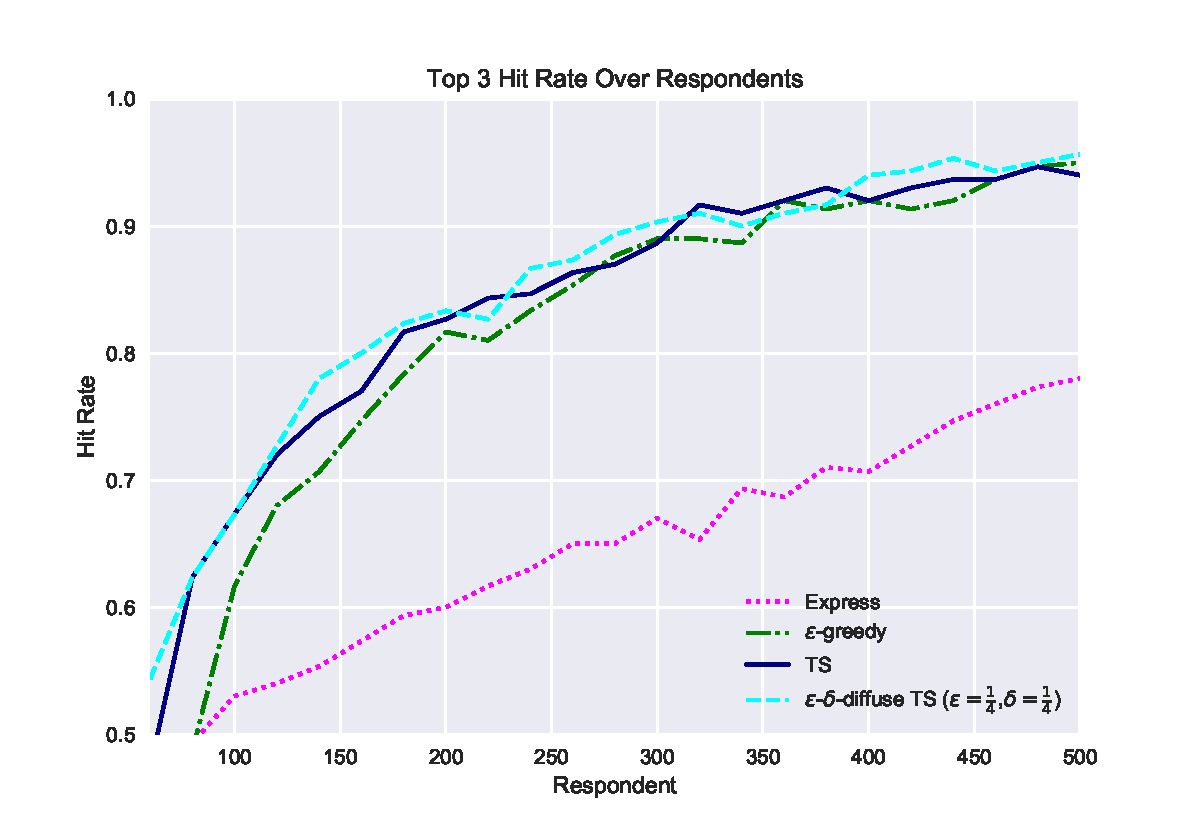
\includegraphics[width=.8\textwidth]{plots/hr120v20k3.pdf} }}%
    \qquad
    \subfloat[Top 10]{{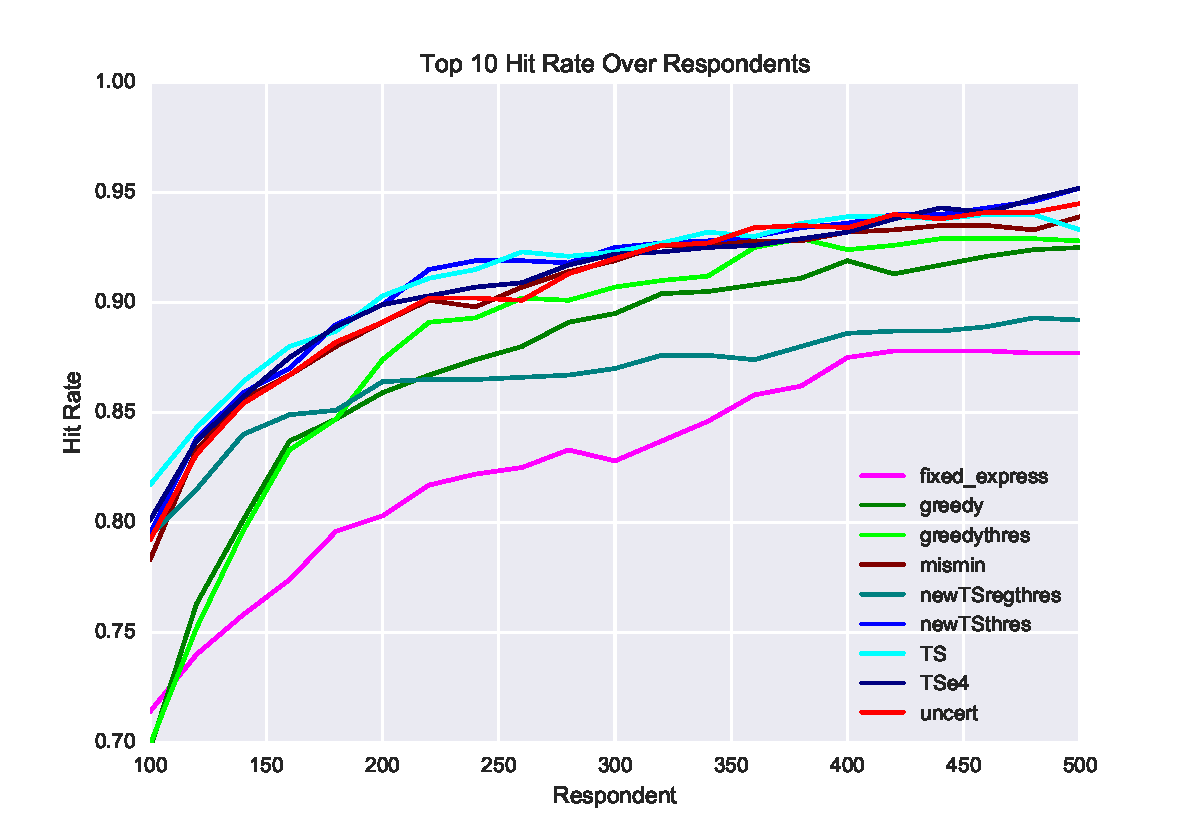
\includegraphics[width=.8\textwidth]{plots/hr120v20k10.pdf} }}%
	\end{center}
\end{figure}


\begin{figure}%
    \caption{The plot shows hit rates for top $k=\{20,40\}$ with 120 items.}%
    \label{fig:K120_L20_k20hit_k40hit}%
 	\begin{center}
    \subfloat[Top 20]{{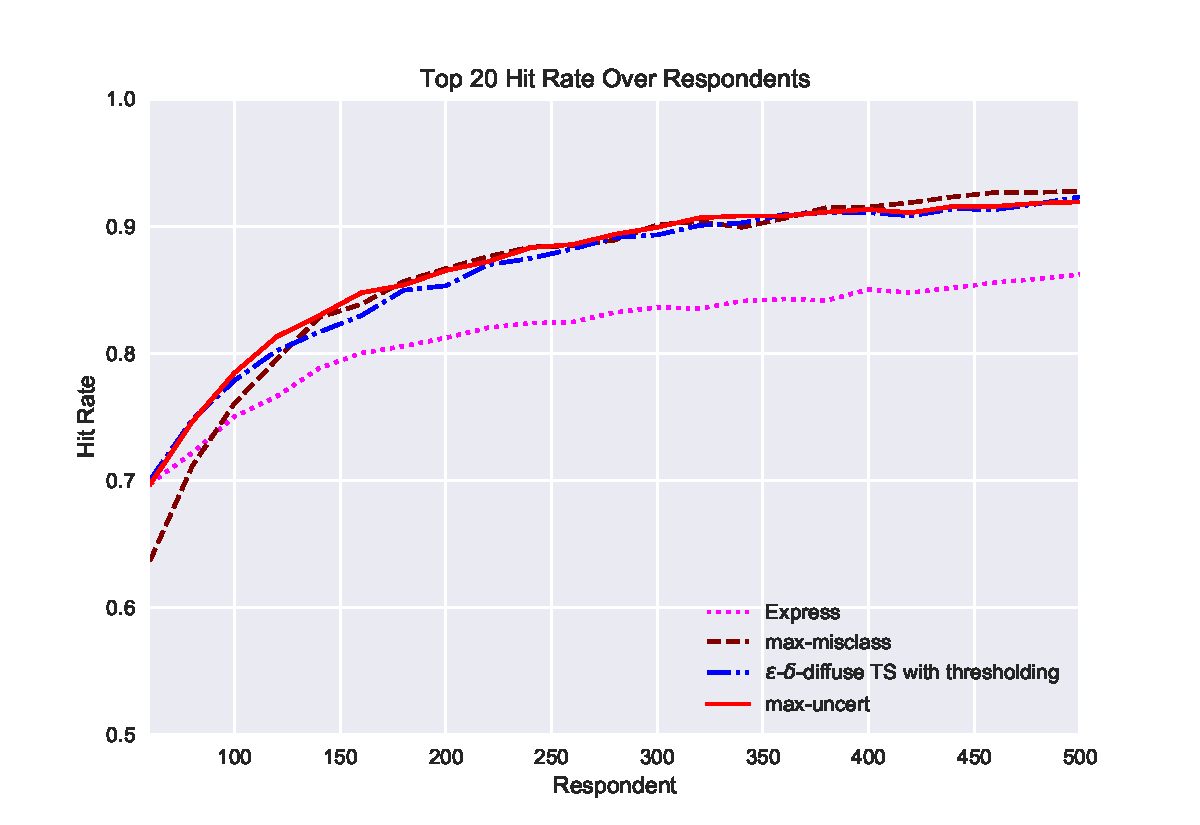
\includegraphics[width=.8\textwidth]{plots/hr120v20k20.pdf} }}%
    \qquad
    \subfloat[Top 40]{{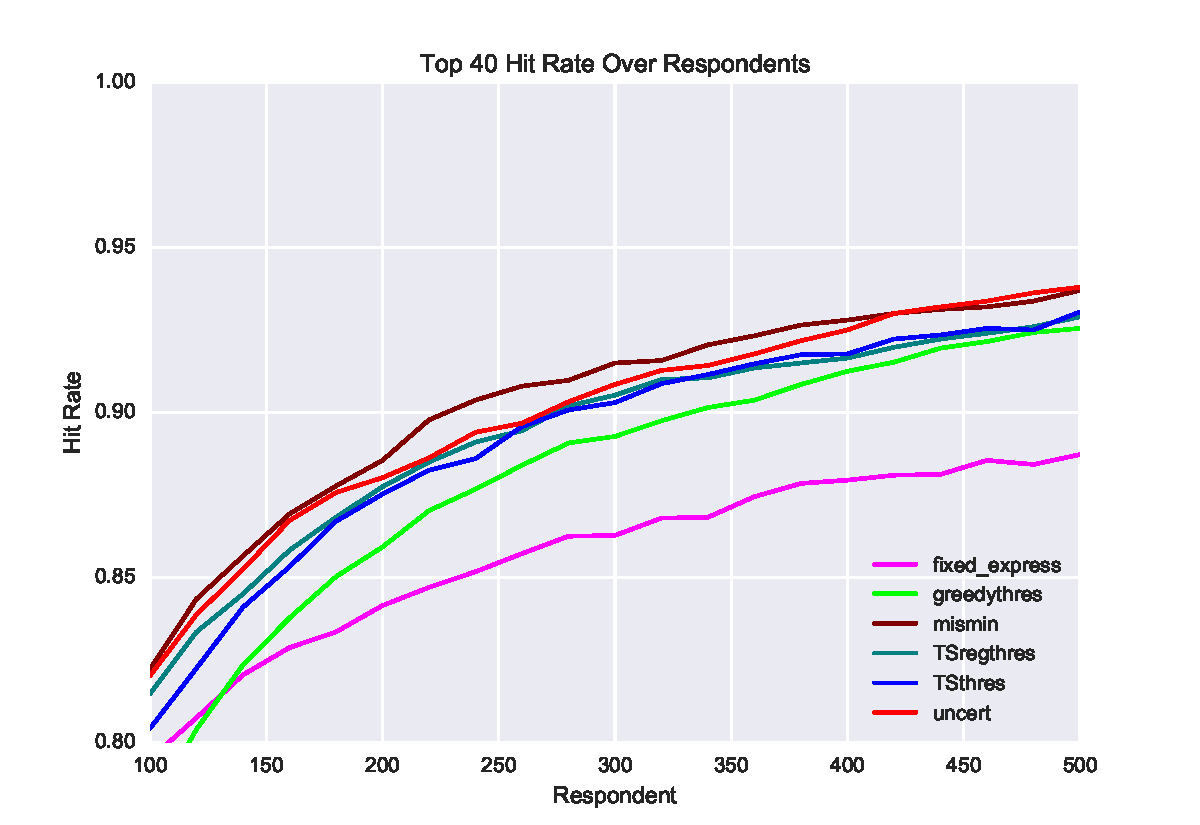
\includegraphics[width=.8\textwidth]{plots/hr120v20k40.pdf} }}%
    \end{center}
\end{figure}


% \begin{figure}
% \caption{3 Hit Rate with 120 items}
% 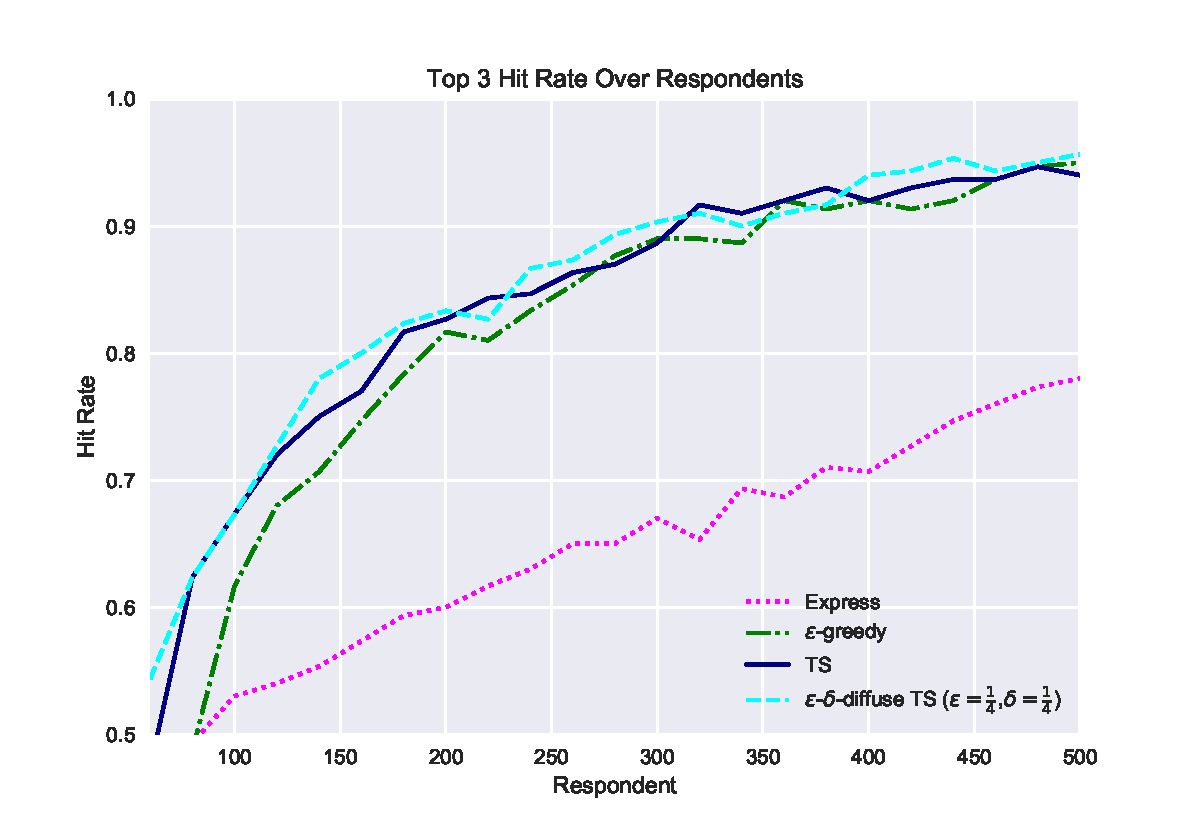
\includegraphics[width=1\textwidth]{plots/hr120v20k3.pdf}
% \label{fig:3hit}
% \end{figure}
% \begin{figure}
% \caption{10 Hit Rate with 120 items}
% 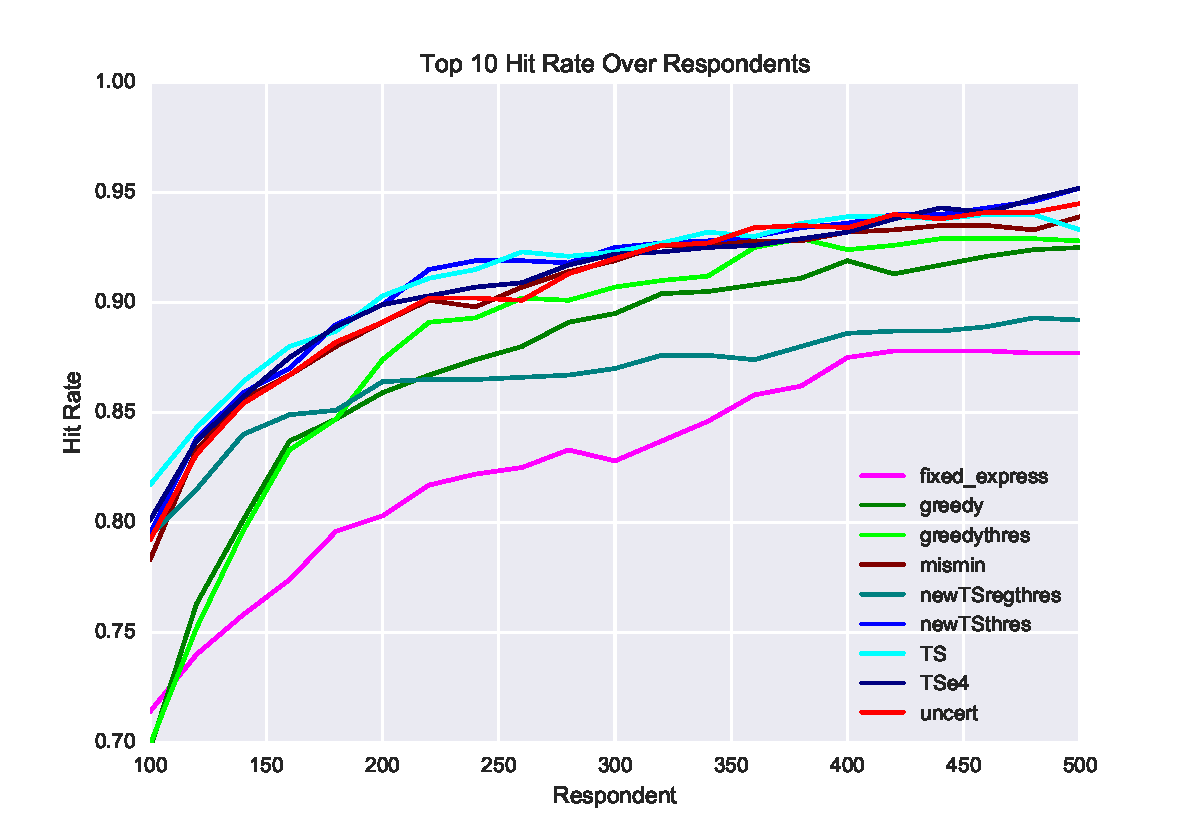
\includegraphics[width=1\textwidth]{plots/hr120v20k10.pdf}
% \label{fig:10hit}
% \end{figure}

% \begin{figure}
% \caption{20 Hit Rate with 120 items}
% 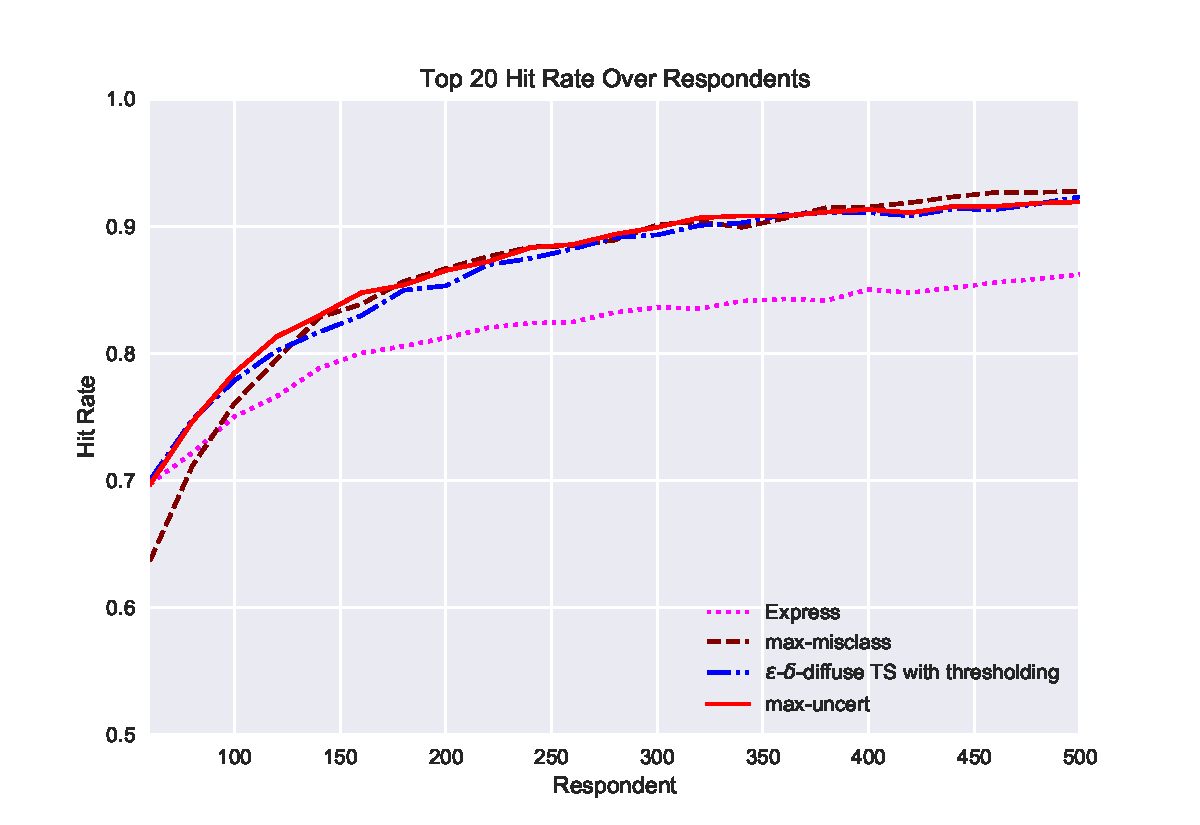
\includegraphics[width=1\textwidth]{plots/hr120v20k20.pdf}
% \label{fig:20hit}
% \end{figure}
% \begin{figure}
% \caption{40 Hit Rate with 120 items}
% 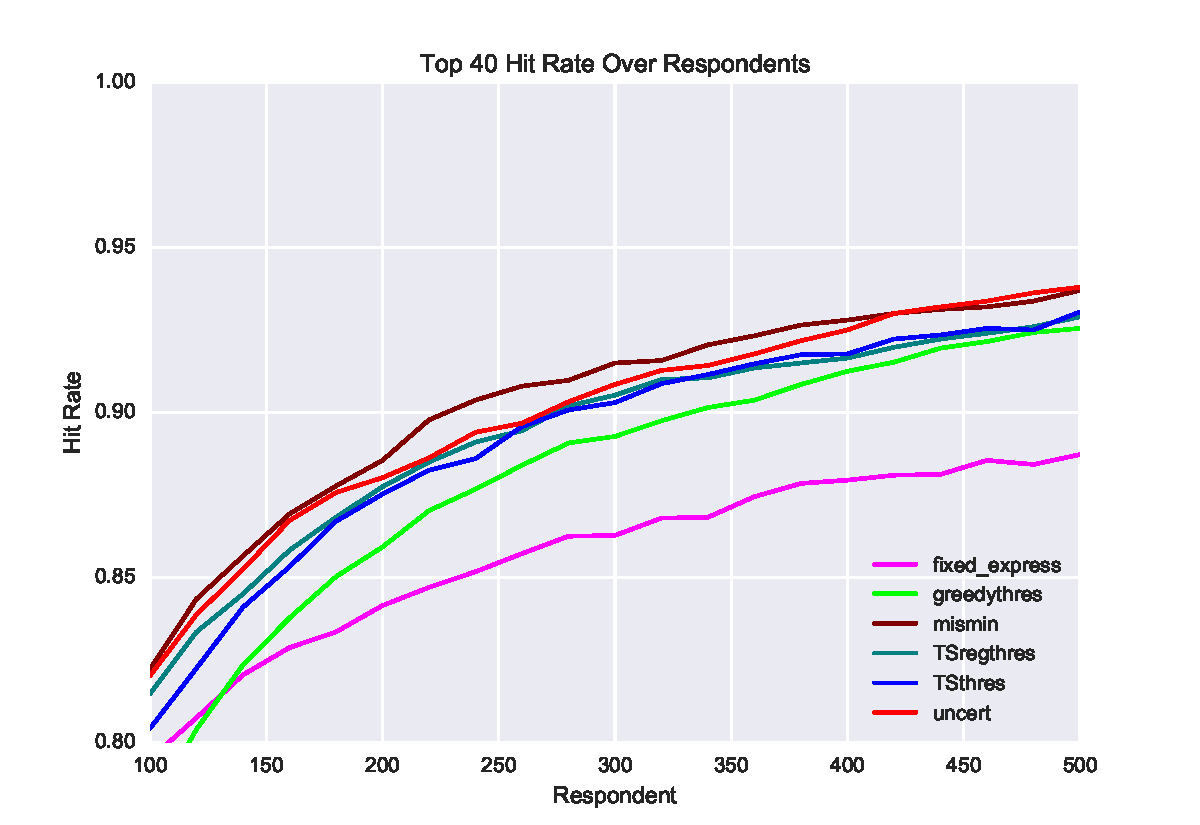
\includegraphics[width=1\textwidth]{plots/hr120v20k40.pdf}
% \label{fig:40hit}
% \end{figure}

\begin{table}
\caption{Top k Hit Rate at 260th and 500th Respondent with 120 Items}
\label{table:at_260_500}
\begin{center}
\begin{tabular}{llllllllll}
\hline 
\hline
\multicolumn{10}{l}{(a) After 260 respondents}\\
k &  \fixedexpressS&\egreedyS&\egreedythresS&\tsS&\edtsS&\tsthresS&\edtsthresS& \misminS& \uncertS \\ \hline
  3 & 0.65 &   0.85 &  0.86 &   0.86 & 0.87 & 0.78 & 0.86 &    0.88 &   0.84 \\
  10 &  0.83 &   0.88 & 0.90 &   0.92 & 0.91 & 0.87 & 0.92 &    0.91 &   0.90 \\
  20 & 0.82 & 0.78 &  0.86 & 0.83 & 0.82 & 0.86 & 0.88 &  0.88 &   0.89 \\  
  40 &  0.86 &   NA &  0.88 &  NA & NA & 0.89 & 0.90 &  0.91 &   0.90 \\
\hline
\hline
\end{tabular}
\begin{tabular}{llllllllll}
\multicolumn{10}{l}{(b) After 500 respondents}\\
k &  \fixedexpressS&\egreedyS&\egreedythresS&\tsS&\edtsS&\tsthresS&\edtsthresS& \misminS& \uncertS  \\
\hline
   3 & 0.78 &   0.95 & 0.93 & 0.94 & 0.96 & 0.83 & 0.97 &    0.95 &   0.94 \\
  10 &  0.88 &   0.93 &  0.93 &   0.93 & 0.95 & 0.89 & 0.95 &    0.94 &   0.95 \\  
  20 &  0.86 &   0.83 & 0.91 &  0.86 & 0.87 & 0.89 & 0.92 &  0.93 &   0.92 \\ 
  40 &  0.89 &   NA & 0.93 & NA & NA & 0.92 &  0.94 & 0.94 & 0.94 \\
\hline 
\hline
\end{tabular}
\end{center}
\end{table}

% \begin{table}
% \caption{Top k Hit Rate for Various Algorithms at the 260th Respondent with 120 Items}
% \label{table:at260}
% \begin{center}
% \begin{tabular}{llllllllll}
% \hline   k &  fixed\_express &  greedy &  greedythres &  mismin &    TS &  TSe4 &  TSregthres &  TSthres &  uncert \\ \hline  3 &          0.650 &   0.853 &        0.860 &   0.883 & 0.863 & 0.873 &       0.850 &    0.893 &   0.840 \\  10 &          0.825 &   0.880 &        0.902 &   0.907 & 0.923 & 0.909 &       0.909 &    0.907 &   0.901 \\  20 &          0.824 &   0.784 &        0.863 &   0.885 & 0.825 & 0.820 &       0.869 &    0.879 &   0.886 \\  40 &          0.857 &   NA &        0.884 &   0.908 & NA & NA &       0.895 &    0.888 &   0.897\end{tabular}
% \end{center}
% \end{table}

% \begin{table}
% \caption{Top k Hit Rate for Various Algorithms at the 500th Respondent with 120 Items}
% \label{table:at500}
% \begin{center}
% \begin{tabular}{llllllllll}
% \hline   k &  fixed\_express &  greedy &  greedythres &  mismin &    TS &  TSe4 &  TSregthres &  TSthres &  uncert \\ \hline   3 &          0.780 &   0.950 &        0.933 &   0.950 & 0.940 & 0.957 &       0.917 &    0.947 &   0.943 \\  10 &          0.877 &   0.925 &        0.928 &   0.939 & 0.933 & 0.952 &       0.940 &    0.947 &   0.945 \\  20 &          0.862 &   0.827 &        0.914 &   0.928 & 0.863 & 0.868 &       0.916 &    0.914 &   0.919 \\  40 &          0.887 &   NA &        0.926 &   0.937 & NA & NA &       0.929 &    0.927 &   0.938 \end{tabular}
% \end{center}
% \end{table}

Our results show algorithm performance depends on the hit rate measure relative to the number of items selected ($k$ versus $\numperset$). For $k \ge L$, the best performers are Greatest Uncertainty with random perturbations (\uncert) and Misclassification Minimization with random perturbations (\mismin). The methods perform nearly as well as the best algorithms for $k < L$, $\epsilon$-diffuse Thompson Sampling with thresholding (\edtsthres) and without thresholding (\edts).

TS alone has its limits---it is constructed to select the best items (and eventually, only the best item), so it performs well identifying a small number of items ($k=3,10$). TS is not suited for the active learning problem, especially when identifying a larger top set, e.g., when a high hit rate for all items in the survey is required ($k=L=20$). While the \edts algorithm adds exploration to improve performance, it does not direct resources toward the areas of high uncertainty at the decision boundary.

\begin{figure}%
    \caption{The frequency of the selected survey item is shown for \edts and \edtsthres.}%
    \label{fig:Frequency}%
 	\begin{center}
    \subfloat[]{{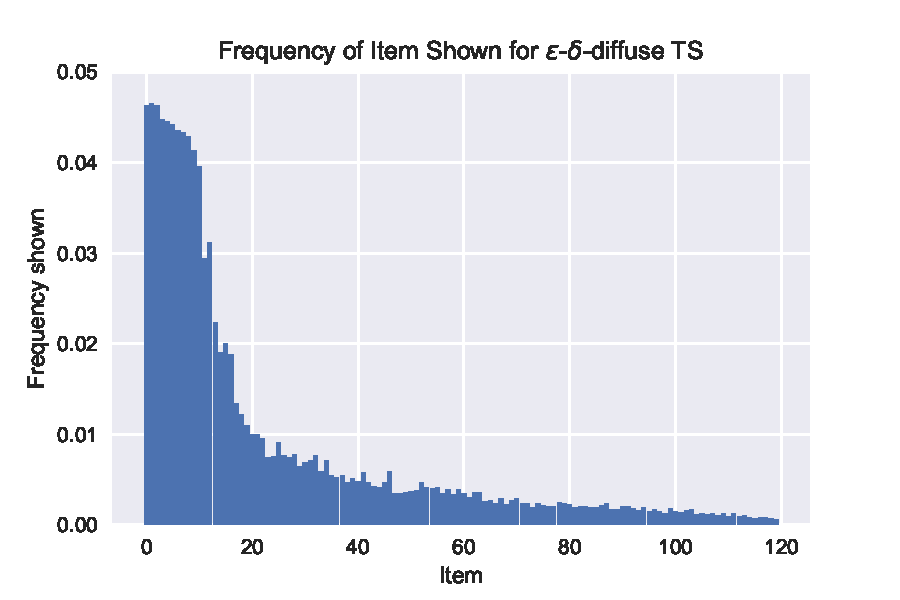
\includegraphics[width=.8\textwidth]{plots/edTSfreq.pdf} }}%
    \qquad
    \subfloat[]{{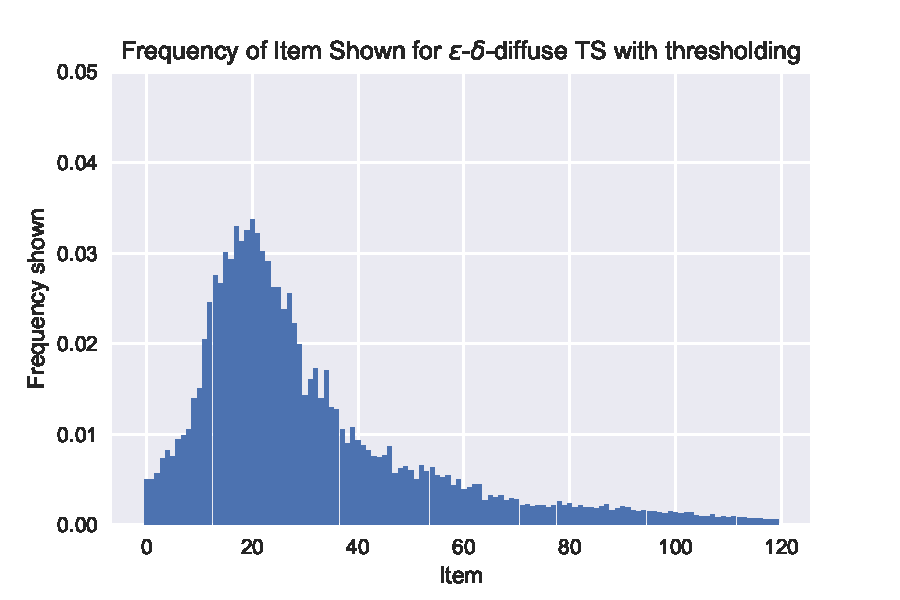
\includegraphics[width=.8\textwidth]{plots/edTSthresfreq.pdf} }}%
	\end{center}
\end{figure}

Why do the threshold-based algorithms, \edtsthres, \uncert, and \mismin, outperform those without thresholds? Imagine showing three items out of six (A, B, C, D, E, and F) to a respondent. We want to identify the top three items. Let A, B, C, D, E, and F be the utility order. We are certain A and B are in the top three, and E and F are not. An algorithm without thresholding would pick A, B, and either C or D. A will be chosen as the best item, and C or D will be chosen as the worst, giving us no new information. An algorithm with thresholding will pick C, D, and either B or E. In either case, the respondent will be forced to compare C and D, providing information about which is in the top three. This is illustrated in Figure \ref{fig:Frequency}, where \edts focuses on the top items and \edtsthres provides more of a spread and focuses on items near rank 20.

% \eric{Add a Takeaway from each section beginning here.} In conclusion, \textbf{we find ... }

\section{Robustness tests} \label{sec:robust}

\subsection{Misinformed Starts}

%\alexander{Look at hr120v20k3moremis1top10.pdf, hr120v20k3moremis2top10.pdf, hr120v20k3moremis2top5.pdf, hr120v20k3moremis1top5.pdf, and see if you want to add in those results (for the 1st 150 respondents percentile of top 3 items is (resp number)/2)}

What would happen if the first 50 respondents to a survey are not representative of the sample's average preferences?

For the simulations reported in table \ref{table:120mis}, the first 50 robotic respondents mimic randomly drawn human vectors of utilities as before. However, they are manipulated to behave as if the true top three preferred items are nearly the worst in preference. (We set the utilities for the population's top three true items equal to the bottom 25th percentile for each respondent).  After the misinformed start, the remaining respondents are well-behaved, drawn using bootstrap sampling, with true individual-level preferences as given in the original P\&G dataset.

\begin{table}
\caption{Top 3 Hit Rate at 260th and 500th Respondent with 120 Items and Misinformed Start}
\begin{tabular}{llllllllll}
\hline   Resp &  \fixedexpressS&\egreedyS&\egreedythresS&\tsS&\edtsS&\tsthresS&\edtsthresS& \misminS& \uncertS   \\ \hline    260 &   0.09 &   0.30 & 0.24 & 0.07  & 0.35 & 0.07 &  0.36 & 0.25 &   0.27 \\
  500 &  0.25 &   0.57 &  0.49 &  0.13 & 0.54 &   0.1 &    0.64 & 0.54 &  0.50  \end{tabular}
\begin{center}
\label{table:120mis}
\end{center}
\end{table}

The misinformed start simulation presents a situation worse than anything marketers might see in practice and suggests robustness to non-stationarity in preference or respondent self-selection during the sampling window.

We create 50 misinforming early responders because in practice we are not guaranteed the first responders represent a fair and representative population draw. Depending on how rapidly we invite a panel of respondents, the first 50 may share some atypical characteristics (e.g., anxious, available to take the survey at launch).

We illustrate the robustness in Table \ref{table:120mis}. The standard Bandit MaxDiff TS approaches perform worse than the Fixed Express MaxDiff algorithm with misinformed starts. The added randomness in the Bandit MaxDiff $\epsilon$-diffuse TS approach, as well as in the other methods, allows it to continue investigating the value of lesser chosen items among later respondents.

\subsection{Increasing Items}
\begin{table}
\caption{Top k Hit Rate at 260th Respondent with 300 Items}
\begin{center}
\begin{tabular}{lllllllllll}
\hline   k &  \fixedexpressS & \egreedyS&\egreedythresS&\tsS&\edtsS&\tsthresS&\edtsthresS& \misminS& \uncertS \\ \hline 
3&   0.31 &   0.59 & 0.48 & 0.60 &  0.64 & 0.54 & 0.65 & 0.54 &   0.58 \\ 
10 & 0.46 &   0.61 & 0.54 & 0.63  & 0.66 & 0.58 & 0.68 & 0.68  &   0.69 \\ 
20 & 0.55 &   0.60 & 0.59 &  0.61 & 0.66 & 0.59 & 0.71 &       0.72 &   0.72\\ 
40 & 0.62 &   NA & 0.62 & NA &  NA & 0.64 & 0.70 & 0.71 & 0.72 \end{tabular}
\end{center}
\label{table:300at260}
\end{table}

\begin{table}
\caption{Top k Hit Rate at 500th Respondent with 300 Items}
\begin{center}
\begin{tabular}{lllllllllll}
\hline   k &  \fixedexpressS & \egreedyS&\egreedythresS&\tsS&\edtsS&\tsthresS&\edtsthresS& \misminS& \uncertS  \\ \hline  
3 & 0.39 &  0.76 & 0.75 & 0.72 & 0.79 & 0.61 &  0.80 &  0.77 &0.78 \\
10 &  0.58 &   0.76 & 0.72 & 0.70 & 0.78 & 0.63 & 0.79 & 0.79 &   0.79\\
20 & 0.68 & 0.72 & 0.76 & 0.67 & 0.76 &  0.63 & 0.82 & 0.84 &    0.85 \\ 
40 & 0.72 &   NA & 0.75 & NA & NA & 0.69 & 0.80 &0.81 & 0.83 \end{tabular}
\end{center}
\label{table:300at500}
\end{table}
Would the benefits of adaptive MaxDiff algorithms observed with 120 items hold for 300 items? While no dataset of utilities from human respondents on 300 possible product features or benefits is available, we generate a data by leveraging the 120-item set provided by P\&G. To generate preferences across an additional 180 items, we combine pairs of existing items according to a randomly distributed weighting scheme, with additional random variation added. The result is a 300-item MaxDiff dataset based on the original preferences of 981 respondents.

The advantages seen in the 120-item results are improved using 300 items. Tables \ref{table:300at260} and \ref{table:300at500} show the well-informed start results. The adaptive approaches show substantial gains over the Fixed Express MaxDiff approach on the top-3, -10, -20, and -40 hit rate criterion.

\subsection{Decreasing Items}

\begin{table}
\caption{Top k Hit Rate at 260th Respondent with 40 Items}
\begin{center}
\begin{tabular}{llllllllll}
\hline   k &  \fixedexpressS & \egreedyS&\egreedythresS&\tsS&\edtsS&\tsthresS&\edtsthresS& \misminS& \uncertS  \\ \hline  3 & 0.90 & 0.97 &  0.97 &  0.97 & 0.97 & 0.97 &  0.96 & 0.94 &  0.94 \\  10 & 0.87 & 0.90 & 0.91 &  0.93 & 0.91 & 0.91 & 0.91 & 0.91 &  0.92  \end{tabular}
\end{center}
\label{table:40at260}
\end{table}

\begin{table}
\caption{Top k Hit Rate at 500th Respondent with 40 Items}
\begin{center}
\begin{tabular}{llllllllll}
\hline   k &  \fixedexpressS & \egreedyS&\egreedythresS&\tsS&\edtsS&\tsthresS&\edtsthresS& \misminS& \uncertS \\ \hline    
3 & 0.93 & 0.99 & 0.99 & 0.99 & 0.99 & 0.98 & 0.98 & 0.98 &  0.99 \\  10 & 0.90 &   0.92 &  0.93  & 0.94 & 0.94 & 0.93 &    0.92 & 0.93 &  0.93 \end{tabular}
\end{center}
\label{table:40at500}
\end{table}
How do the adaptive models perform using a more traditional MaxDiff set of 40 items? Using a random 40-item subset from the original set of 120 items, the Express MaxDiff design shows each item to every other respondent on average, more than in larger item cases. Still, the adaptive MaxDiff approaches perform better than traditional MaxDiff models (Table \ref{table:40at260}).

%By reducing the number of items to 40 and changing the number of tasks to 12, the fixed express design can now show each item an average of 1.5 times per respondent, which is much less sparse than in larger item cases.\\

\subsection{Simulated Data Set}
\begin{table}
\caption{Top k Hit Rate at 260th Respondent with Simulated Data Set}
\begin{center}
\begin{tabular}{llllllllll}
\hline   k &  \fixedexpressS & \egreedyS&\egreedythresS&\tsS&\edtsS&\tsthresS&\edtsthresS& \misminS& \uncertS \\\hline  10 & 0.77 &   0.88 & 0.88  & 0.87&0.89 & 	0.88&0.89 & 0.89 &  0.88 \\  20 &  0.87 &  0.86 &   0.92  & 0.88&0.90 &  	0.93&0.94&  0.93 &  0.93 \end{tabular}
\end{center}
\label{table:nice260}
\end{table}

\begin{table}
\caption{Top k Hit Rate at 500th Respondent with Simulated Data Set}
\begin{center}
\begin{tabular}{llllllllll}
\hline   k &  \fixedexpressS & \egreedyS&\egreedythresS&\tsS&\edtsS&\tsthresS&\edtsthresS& \misminS& \uncertS  \\\hline    10 & 0.85&0.92&0.92 & 0.93&0.94 & 0.92&0.94&0.93 &   0.93 \\  20 & 0.90&0.90&0.95& 0.90 &0.93 & 0.95&0.96 &0.96& 0.96 
\end{tabular}
\end{center}
\label{table:nice500}
\end{table}

As a baseline for a simulated dataset, we sample $\theta_i$ from a uniform distribution for $i=1,\ldots,100$. Each respondent preference utility is sampled from a normal distribution with mean $\theta_i$ and variance 1. The rankings for each respondent are highly correlated. We take the top $k$ highest mean preference scores across the respondents to be the top $k$ true items. The results are shown in Tables \ref{table:nice260} and \ref{table:nice500}.

\subsection{Alternate Data Set}

\begin{table}
\caption{Top k Hit Rate at 250th and 500th Respondent with 86 Items from Skim Group}
\label{table:skim}
\begin{center}
\begin{tabular}{llllllllll}
\hline 
\hline
\multicolumn{10}{l}{(a) After 250 respondents}\\
k &  \fixedexpressS&\egreedyS&\egreedythresS&\tsS&\edtsS&\tsthresS&\edtsthresS& \misminS& \uncertS \\ \hline
  3 & 0.90 &   1.00 &  NA &   0.97 & 0.99 & NA & NA &    0.98 &   0.97 \\
  10 &  0.88 &   0.90 & 0.92 &   0.91 & 0.92 & 0.89 & 0.91 &    0.93 &   0.92 \\
  20 & 0.91 & 0.87 &  0.96 & 0.86 & 0.91 & 0.92 & 0.96 &  0.96 &   0.92 \\  
  40 &  0.92 &   NA &  0.95 &  NA & NA & 0.94 & 0.95 &  0.96 &   0.95 \\
\hline
\hline
\end{tabular}
\begin{tabular}{llllllllll}
\multicolumn{10}{l}{(b) After 500 respondents}\\
k &  \fixedexpressS&\egreedyS&\egreedythresS&\tsS&\edtsS&\tsthresS&\edtsthresS& \misminS& \uncertS  \\
\hline
   3 & 0.94 & 1.00 & NA & 0.98 & 1.00 & NA & NA & 1.00 &   0.99 \\
  10 &  0.91 &   0.92 &  0.93 &   0.92 & 0.93 & 0.90 & 0.93 &    0.93 &   0.94 \\  
  20 &  0.94 &   0.90 & 0.98 &  0.89 & 0.94 & 0.94 & 0.98 &  0.98 &   0.98 \\ 
  40 &  0.95 &   NA & 0.97 & NA & NA & 0.96 &  0.97 & 0.97 & 0.97 \\
\hline 
\hline
\end{tabular}
\end{center}
\end{table}

We use data from a study of claims for cleaning products as a skim group. The simulation parameters are the same as in the P\&G study, except we make the batch size 10 rather than 20. The results are shown in Table \ref{table:skim}.

\section{True Utility as Hit-Rate Generalization}
\begin{table}
\caption{PTU for Various $S$ for P\&G Data Top 3}
\begin{center}
\begin{tabular}{c | c }
$S$& Percent True Utility \\
\hline
\{1,2,3\}& 1.0 \\
\{1,2,4\}&.973 \\
\{1,2,5\}&.948 \\
\{1,3,4\}&.934 \\
\{1,3,5\}&.910 \\
\{1,4,5\}&.882 \\
\{2,3,4\}&.922 \\
\{2,3,5\}&.897 \\
\{2,4,5\}&.870 \\
\{3,4,5\}&.831 \\
\hline
\end{tabular}
\end{center}
\label{table:PTU}
\end{table}
To differentiate between an algorithm that puts the top nine items and the 11th item in the top 10 and one that puts the top nine items and the 40th item in the top 10, we use percent true utility (PTU).

For a set $S$, the exponential weighted utility is \[\mu_S=\sum_{x \in S}b(x)=\sum_{x \in S}e^{u(x)},\]
and PTU is the exponential weighted true utility of the top $k$ items the robotic respondents identify over the maximum exponential weighted true utility that could be attained with $k$ items. If $\tilde{S}$ are the top $k$ items and $S$ is the current estimate of the top $k$ items, PTU is 
\[
\frac{\mu_S}{\mu_{\tilde{S}}}.
\]
This generalization of hit rate can be used to differentiate the algorithms, though the results are difficult to interpret. Table \ref{table:PTU} shows PTU for various data subsets.
\begin{figure}
\caption{The plots show percent true utility for the top 20 of 120 items.}
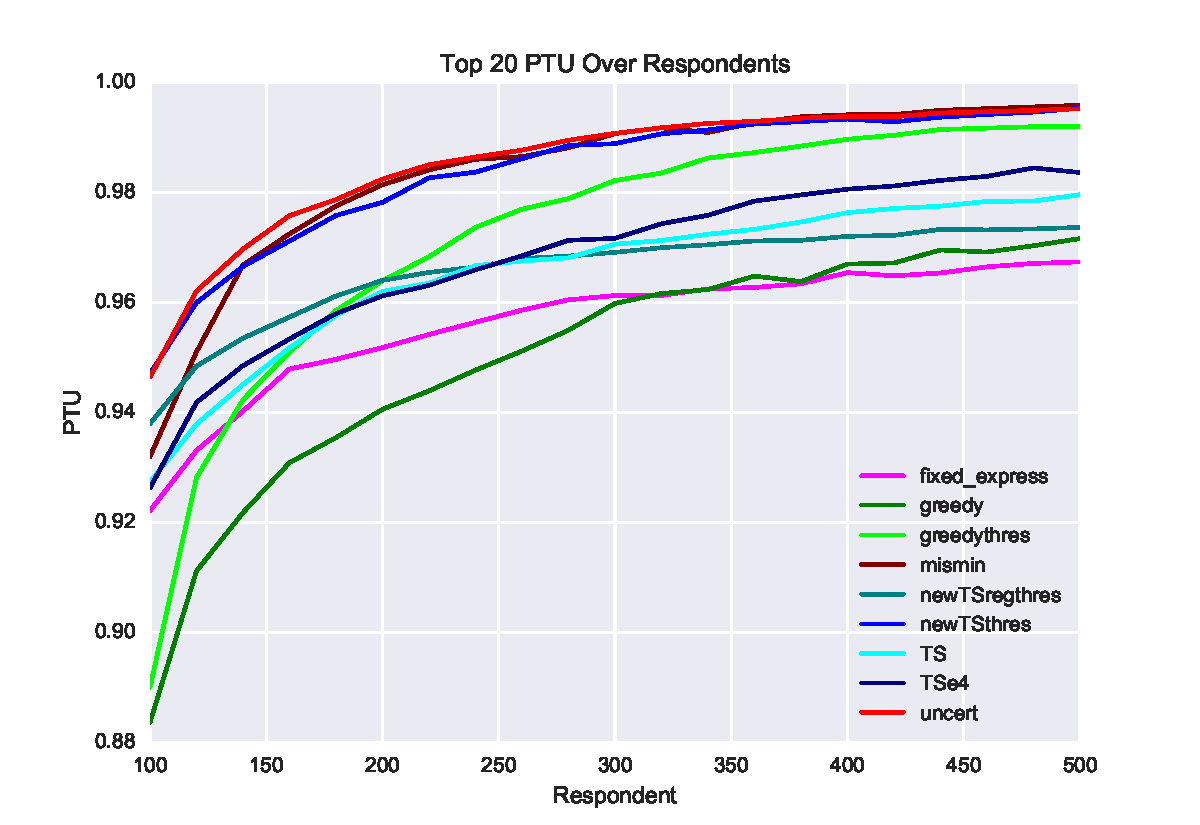
\includegraphics[width=1\textwidth]{plots/PTU120v20k20.pdf}
\label{fig:20util}
\end{figure}
For $k=20$, hit rate is similar for the Fixed Express, TS, and \edts models. Using $k=20$ PTU, we find \edts has a slight edge over TS and Fixed Express (Figure \ref{fig:20util}). Both TS approaches place more appropriately ranked items in the top 20 than Fixed Express.

\section{Stopping Rules: Posterior Distribution Regret and Value Remaining}

Almost all our results show diminishing algorithm performance at some point as we administer more surveys. Therefore, it becomes inefficient to continue surveying after a certain number of respondents. In practice, we do not know this point a priori. So how do we know when to stop?

Adapted from~\cite{scott2015multi} and~\cite{scott2010modern} for multi-armed bandit problem solving, the value remaining in the experiment is the posterior distribution of $\frac{\mu_{S^*}-\mu_{S}}{\mu_{S}}$, where $\mu_{S^*}$ is the largest value of the exponential weighted utility and $\mu_{S}$ is the exponential weighted utility of the set most likely to be optimal, denoted $S$. We take $n$ Bayes Bootstrap draws from the posterior, letting $\mu_{S^*}^{m}$ be the maximum exponential weighted utility of draw $m$ and $\mu_{S}^{m}$ be the utility using draw $m$ from set $S$. We let $\Delta^{m}=\frac{\mu^m_{S^*}-\mu^m_{S}}{\mu^m_{S}}$.

\begin{table}
\begin{center}
\caption{Draws of Items' Exponential Utility after 100 Iterations}
\label{table:data}
\begin{tabular}{l | c c c c c c c c}
& \multicolumn{8}{c}{Current belief: rank order of items by utility} \\
& 1st &  2nd  &  3rd  &  4th &  5th & 6th & 7th &  8th \\
\hline
% \multicolumn{9}{l}{Posterior draws of utility} \\
Draw 1 & 4.02 &  3.50 &  5.08 & 4.16&  4.22 & 4.41 & 3.65 &  3.27 \\
Draw 2 &4.18 & 4.72 & 3.49 & 3.48 & 3.63 & 3.60 & 3.56 &  3.70 \\
Draw 3 &4.81 & 5.23 & 5.04 &  3.96 &  4.17 & 4.37 &  3.58 & 2.99 \\ 
\end{tabular}
\end{center}
\end{table}

\begin{figure}
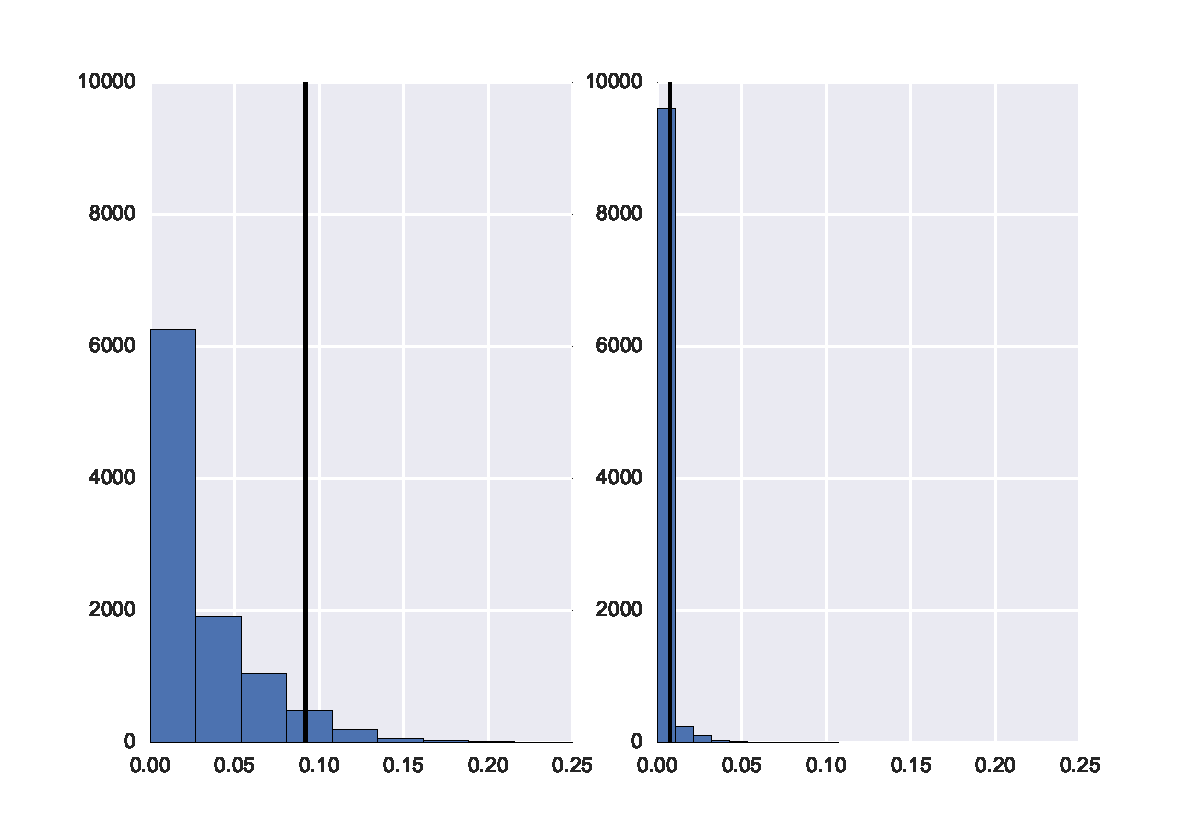
\includegraphics[width=1\linewidth]{plots/valremhist.pdf}
\caption{Two histograms of $\Delta$ are shown. At left, after 100 iterations, the potential value remaining is 0.092. At right, after 220 iterations, the potential value remaining is 0.008.}
\label{fig:data}
\end{figure}

Table \ref{table:data} shows the exponential weighted utility of a single item. The columns are in current rank order and show the top eight utilities. $S$ is the set containing the current first, second, and third ranked items. Then, $\mu^1_{S}=4.02+3.50+5.08=12.6$ and $\mu_{S^*}^{1}=5.08+4.41+4.16=13.65$, so $\Delta^{1}=\frac{13.65-12.6}{12.6}=.083$. Likewise, $\Delta^{2}=\frac{12.6-12.39}{12.39}=.017$ and $\Delta^{3}=\frac{15.08-15.08}{15.08}=0$. (Note $\Delta^m=0$ when $S$ contains the top utilities.) The histogram of $\Delta$ after 100 iterations and 220 iterations is shown in figure \ref{fig:data}.

The potential value remaining (PVR) is the 95 quantile of the distribution $\Delta$ (Figure \ref{fig:data}). After 100 iterations, PVR is 0.092. While we do not know the utility of $S$, we know an alternative set might perform better by as much as 9.2\%.

 %\alexander{Replace this plot with stophisted02.pdf stophistprob02.pdf and stophistTSgr02.pdf}

\begin{figure}
\caption{Average stopping times are shown with various thresholds.}
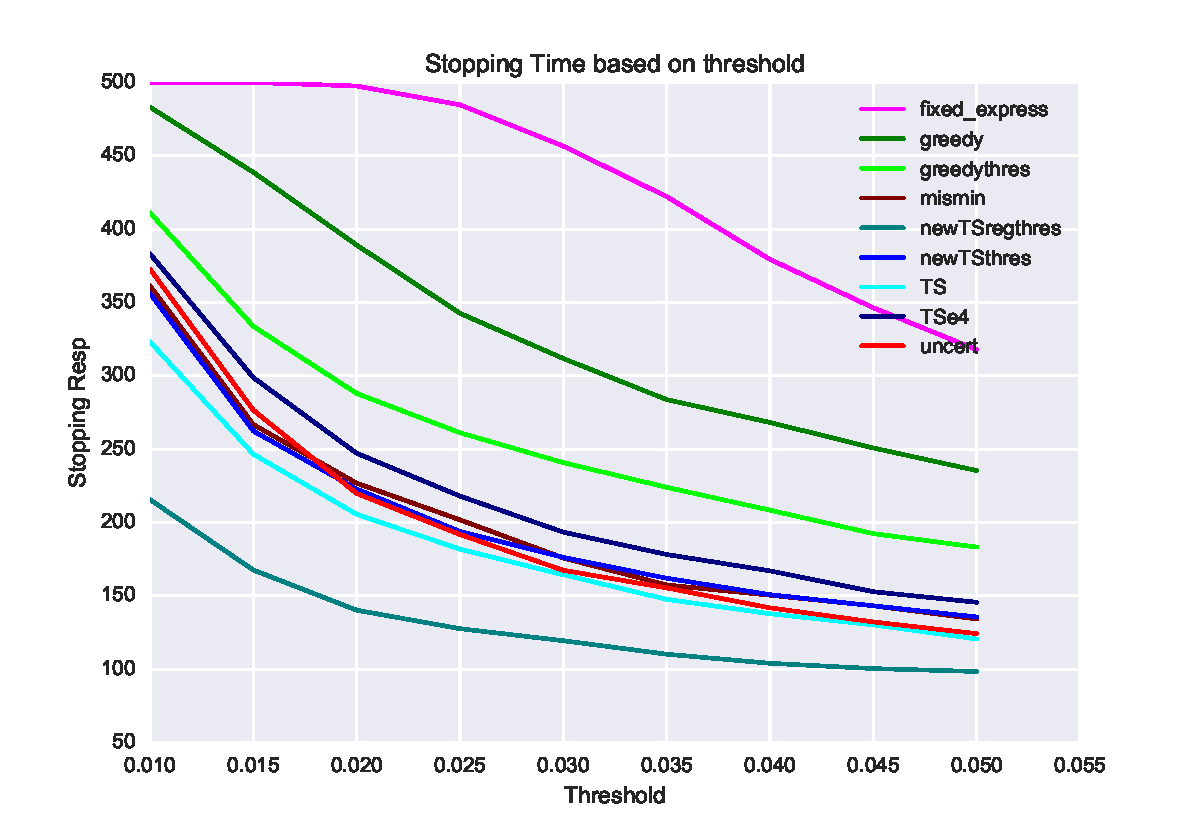
\includegraphics[width=1\textwidth]{plots/stoppingtimes.pdf}
\label{fig:st}
\end{figure}
\begin{table}
\begin{center}
\caption{Average Stopping Time and Hit Rate With PVR Threshold 0.05 for Top 10 Items}
\label{table:st5}
\begin{tabular}{llllllllll}
\hline    &  fixed\_express &  greedy &  greedythres &  mismin &    TS &  TSe4 &  TSregthres &  TSthres &  uncert \\\hline  Avg ST  & 318 &   235 & 183 & 134 & 121 & 146 & 	98 &	136 &   124 \\  Avg hr  &  0.854 &  0.88 & 0.852&0.848 & 0.846 & 	0.866 & 0.795 &0.857 &  0.837 \end{tabular}
\end{center}
\caption{Average Stopping Time and Hit Rate With PVR Threshold 0.02 for Top 10 Items}
\label{table:st2}
\end{table}
\begin{table}
\begin{center}
\begin{tabular}{llllllllll}
\hline    &  fixed\_express &  greedy &  greedythres &  mismin &    TS &  TSe4 &  TSregthres &  TSthres &  uncert \\\hline    Avg ST & 498 & 389 & 288 & 227 & 206 & 247 & 140 &223 &  220 \\ Avg hr & 0.893 &0.918&0.902& 	0.911 & 0.907& 0.912 & 0.822&0.911& 0.909\end{tabular}
\end{center}
\end{table}

We might therefore stop administering surveys when PVR drops below a certain threshold. Figure \ref{fig:st} shows the average ending point for different algorithms based on the threshold of finding the top 10 items. Tables \ref{table:st5} and \ref{table:st2} show the average stopping times and hit rates for threshold PVR values of 0.02 and 0.05. In general, higher $k$ values yield smaller PVR values.

%\subsection{Spearman (Rank Ordering) Correlation}
%Both hit rate and percent true utility are invariant under the ordering of the $k$ items. As a final metric we looked at the Spearmen Correlation of the true top $k$. This measures how well the algorithm's ranking of the true top $k$ items matches with the truth. For example if the 

\section{Alternative Sampling}

%\subsection{Changing Exploration Parameters}
%Almost all of the adaptive methods have parameters for all of these methods and the trade off is robustness against heterogeneity in the respondents verses speed of convergence. All the Greatest Uncertainty with random perturbation and Misclassification Minimization with random perturbation $c=\infty$ (or any $c \geq 250$ in the case 120 items showing 20 items to each respondent) is fixed express, and using $c=0$ , $\epsilon$-greedy with $\epsilon=1$, and $\epsilon$-diffuse TS with $\epsilon=1$ and $\delta=0$ are the same sampling scheme as fixed express. Also $\epsilon$-diffuse TS with $\epsilon=0$ is regular TS.  Our recommended ranges for the different parameters are $\frac{1}{5}\leq \epsilon \leq \frac{1}{2}$, $\frac{1}{4}\leq \delta \leq \frac{1}{2}$ and $.01 \leq c \leq 1$.

\subsection{Best, Not Best-Worst}

Adaptive MaxDiff approaches perform best when the researcher is mainly interested in identifying the top few items in a set. Is it valuable in this case to ask respondents to identify the worst item within each MaxDiff set? The value of asking respondents to indicate both their best and worst choices within each set more than compensates for the 40\% additional effort we estimate the questions add to the total interview time when working with human respondents.

In a five item set (A,B,C,D, and E), we have 10 possible two-way comparisons. If we assume A is preferred to B and B is preferred to C and so on, asking respondents to indicate only the best item will let us know A$>$B, A$>$C, A$>$D, and A$>$E (4/10 comparisons). By asking about respondents' least preferred items, we also know B$>$E, C$>$E, and D$>$E (7/10 comparisons), leaving only the order relationship between B, C, and D unknown.

The case of asking for top choices when all respondents have the same preferences aligns with the marked bandit problem outlined by~\cite{simchowitz2016best}, where the authors offer different algorithms for pulling the arms and upper and lower bounds on how many queries it takes to identify the top $k$ items with high probability. 

% \subsection{What about Double Adaptivity?}
% In~\cite{orme2006adaptive}, one of the authors presented a paper on Adaptive MaxDiff that featured within-respondent adaptation rather than what we have shown here in Bandit MaxDiff based on Thompson Sampling, which is an across-respondent adaptive approach. For the within-respondent adaptive procedure, items that a respondent indicates are worst are dropped from further consideration by that same respondent through a round-robin tournament until eventually that respondent's best item is identified.  We thought adding this additional layer of within-respondent adaptivity on top of the Bandit MaxDiff approach could additionally lift its performance.  To our surprise, this double-adaptive approach actually performed worse than Bandit MaxDiff alone in terms of hit rates for the top 3 or 10 items for the sample.  After some head-scratching (and much code checking), we determined that the lack of improvement was due to degree of heterogeneity across the robotic respondents.  For example, if we are interviewing a respondent who doesn't agree much with the overall population regarding which are the top items, it is detrimental to allow that respondent to drop from further consideration (due to judging them worst) what actually are among the globally most preferred items.  It serves the greater good for each respondent to spend increased effort judging among the items that previous respondents on average have judged as potentially best.

\subsection{Asymptotic Distribution vs. Bayesian Bootstrap}

As an alternative to Bayesian Bootstrapping for posterior draws, we can sample from the asymptotic distribution via MLE implied by the estimated mean and standard errors, sampling $u \sim N(\theta,H^{-1})$, where $\theta$ is the minimizer of the negative log-likehood and $H$ is the Hessian of the negative log-likehood evaluated at $\theta$. The sampling methods perform similarly using draws from Bayesian Bootstrapping and asymptotic distribution.

Another method allows for online updates for streaming data without model estimation. MaxDiff tasks yield a number of pairwise comparisons via a single best-worst pair. We can therefore act as if the respondent states all such comparisons and assign a win to the more preferred item and loss to the others. By tallying wins for each item, we can compare win percentages among items that have faced each other and find a noisy measure of underlying utility. Taking win percentage as an average, $\hat{p}_{win}$, we can use its standard error, $se_{win}$, in TS as follows:
\begin{align}
\hat{p}_{k,win} &= n_{k,wins} / n_{trials} \\
\text{se}_{k,win} &= \sqrt{  \frac{ \hat{p}_{k,win} (1-\hat{p}_{k,win}) } {n_{trials}}.  } \\
\end{align}

The mean and variance can be used for sampling from the winning percentages distribution in TS or \edts. For TS, after sampling one $p_{k,win}^{ts}$ for each of the $k=1,\ldots,K$ items independently, we can rank order and identify the top set of values. For \edts, we do this for two different normal distributions, one with $\text{se}_{k,win}$ and one with the inflated standard error, $\delta \text{se}_{k,win}$.

%\subsection{Other Sampling Schemes}
%TO DO: change this section
%In ~\cite{russo2016simple}, the author analyses different Bayesian algorithms for identifying the best arm. One point he makes is that Thompson Sampling is not effective for purely exploration problems. TS leads to oversampling the top item and not getting good enough estimates the second best items to conclude with high enough confidence that the top item is the top item. He gives a variation Top-Two Thompson Sampling which is better for the best-arm identification problem. This is choosing the best arm with probability $\beta$ and choosing the second best arm with probability $1-\beta$. One way to implement this in MaxDiff surveys is top pick the top 30 items and for each item with rank $i$ with probability $1-\beta$ replace that item with the rank $i+30$ ranked item.\\
%While our problem is purely exploration, the nature of MaxDiff survey causes us to show $\numperset$ items to every respondent, putting a limit on how much we are sampling the each item. As a result when $k$ is less $\numperset$ we do not run in to the same estimation problems as in MAB problem. Though as we saw in PVR, adding randomness can improve the speed of parameter estimates in the same spirit as Russo's paper.\\

%\subsection{Thompson Sampling for purely exploration problems}

%\begin{figure}
%\caption{30 Hit Rate with 120 items}
%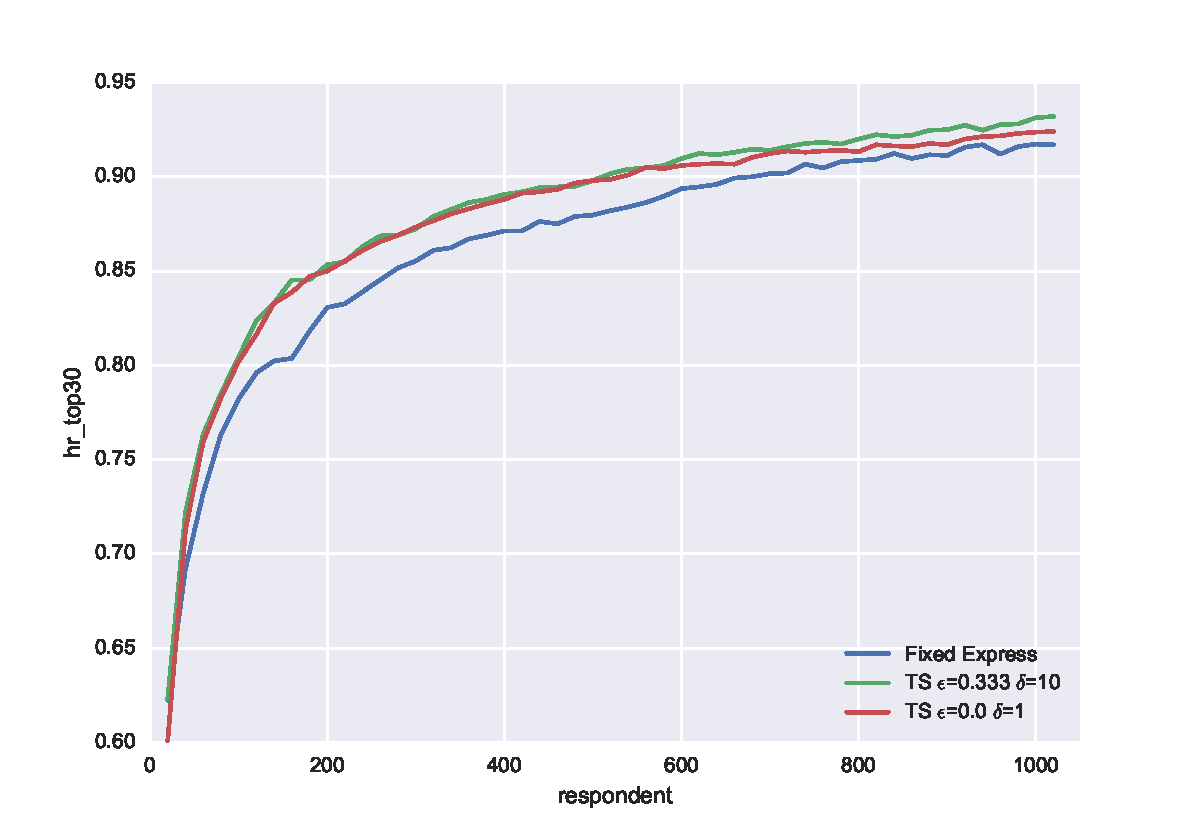
\includegraphics[width=1\textwidth]{plots/30hitrate120show3.pdf}
%\label{fig:30hit}
%\end{figure}
%Consider \ref{fig:30hit}, while MAB methods still gives a edge over fixed sparse the gains are much less. One reason is that TS sampling will  
%at is considered in ~\cite{toubia2007adaptive}, but for a different type of survey. Instead of showing a series of items and ask respondents to pick the best and worst from a list, the survey shows the respondents one item and asked to rate it using the binary choice good or bad. With each query they get information on one item. As a result the authors show fewer items to each respondent. Similar to our approach, the authors devise adaptive approaches that use previous ratings to decide the what items to show the next respondent.  Unlike our approach, they sample items more that are likely to be misclassified by looking at items close to the threshold between top items and bottom items (not top items).\\
%It is interesting to note that their best preforming solution is similar in spirit to our method of $\epsilon$-Diffuse TS. In implementation their method uses a beta distribution and can calculate their score directly instead of taking a sample. They then add noise from a normal distribution to each of the scores and show the top scoring items to the next respondent. Despite the differences, the similarity between their best method and is $\epsilon$-Diffuse TS striking.

\subsection{Sparse MaxDiff vs. Express MaxDiff}
In ~\cite{wirth2012largeset}, the authors compare non-adaptive Sparse MaxDiff and Express MaxDiff. For Fixed Sparse MaxDiff, we show each item to each respondent an equal number of times (if possible). With 120 items, 12 sets and five items per set appear on average $\frac{12*5}{120} = 0.5$ times per respondent. We compare the results using our simulation and find a modest edge in performance for Express MaxDiff---Sparse MaxDiff ending at 85.6\% for a top 10 hit rate and Express MaxDiff ending at 87.7\%.

\section{Conclusions and Future Research}

Idea screening problems not only involve identifying the top set of targets for data collection projects, but they also serve as an illustration of a broader framework. By aligning the process with managerial objectives, we can improve efficiency and scalability for big data collection via choice experiments. Specifically, we improve precision only where it matters for decision making, using a smaller sample size compared to existing methods, and we demonstrate our work's viability empirically with MaxDiff, an increasingly popular and important choice experiment method.

We contribute to the literature and practice by framing choice task data collection as a best arm identification, multi-armed bandit, and active learning problem. During data collection, we adaptively learn preferences to maximize accuracy in identifying the set of items most important to consumers. In practical marketing terms, we are able to identify top preferences quickly and complete data collection projects sooner than with traditional methods, which saves firms money. 

If a firm's main goal is to use MaxDiff to identify the most preferred items among a large population, rather than make individual-level estimates, adaptive MaxDiff approaches can be three times more efficient than standard designs. Firms are potentially wasting 66 cents of each dollar spent on data collection.

Adaptive MaxDiff leverages information from prior respondents to show more effective tradeoffs to later respondents (tending to oversample the highest performers). The algorithms performing well under any choice $k$ include Greatest Uncertainty with random perturbations, Misclassification Minimization with random perturbations, \edts with thresholding, and $\epsilon$-greedy with thresholding. Additionally, \edts works well when $k<L$, and $\epsilon$-greedy works well when $k<<L$.

Even in the face of imposed misinformed starts  and unrepresentative first responders, the adaptive MaxDiff approaches are robust and self-correcting.

Although our simulations involve 120-item and 300-item tests, we expect even greater efficiency gains compared to standard Express MaxDiff designs may occur in MaxDiff studies with 500 or more items. For studies using 40 respondents, our simulation shows a 200\% advantage in efficiency over Fixed MaxDiff designs.

Future research should test our findings using human respondents. Using an adaptive process focusing on comparing best items may result in a more cognitively difficult task than a standard, level-balanced, near-orthogonal approach.  The greater expected within-set utility balance may lead to higher response error, which may counteract some of the benefits of the adaptive approaches.  However, based on previous research by~\cite{orme2006adaptive} employing within-respondent adaptivity, the additional degree of difficulty likely would not entirely counteract the benefits.

This paper introduces a framework that links the conjoint and multi-armed bandit methods of solving large-scale scaling and ranking problems. As adaptive conjoint methods began with aggregate adaptation and progressed to the individual level, we propose an aggregate adaptive approach. Future work could explore methods using fully heterogeneous models and adapting within each individual survey respondent. A partially pooled model might be useful, as it is with other adaptive conjoint methods. 

Our problem solving method relates to existing adaptive conjoint approaches as M-efficiency criterion relate to D-efficiency criterion.  Unlike M-efficiency designs, where the researcher decides the managerial weight of different factors a priori, we seek to learn the weight of each item actively. 

As of this article's publication date, Sawtooth Software does not offer Bandit MaxDiff as a commercial tool. The company is currently testing versions to make available to the public.

% Acknowledgments here
%MKSC_FORMAT% \ACKNOWLEDGMENT
\textbf{Acknowledgments:}
{%
% Enter the text of acknowledgments here
}% Leave this (end of acknowledgment)


% Appendix here
% Options are (1) APPENDIX (with or without general title) or 
%             (2) APPENDICES (if it has more than one unrelated sections)
% Outcomment the appropriate case if necessary
%
% \begin{APPENDIX}{<Title of the Appendix>}
% \end{APPENDIX}
%
%   or 
%
% \begin{APPENDICES}
% \section{<Title of Section A>}
% \section{<Title of Section B>}
% etc
% \end{APPENDICES}

% References here (outcomment the appropriate case) 

% CASE 1: BiBTeX used to constantly update the references 
%   (while the paper is being written).
\bibliographystyle{informs2014} % outcomment this and next line in Case 1
\bibliography{source,activelearning,banditbib,banditpricingbib,mktg_activelearn} % if more than one, comma separated

% CASE 2: BiBTeX used to generate mypaper.bbl (to be further fine tuned)
%\input{mypaper.bbl} % outcomment this line in Case 2

\newpage

\section*{Appendix} 


\begin{figure}
\caption{A 2015 Sawtooth Software customer feedback survey explored the maximum number of items users studied via MaxDiff (top: mean= 40, median=30, maximum=400) and their main purpose in conducting a study with at least 41 items (bottom). } 
\label{fig:max_and_purpose}
\begin{center} 
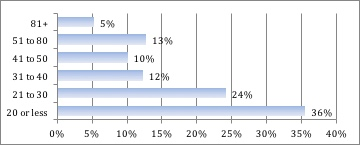
\includegraphics[width=0.7\textwidth]{plots/maxnumstudy}
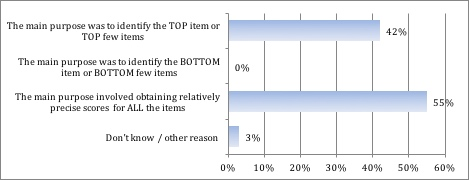
\includegraphics[width=0.7\textwidth]{plots/maxdiffpurpose}
\end{center}
\end{figure}


\subsection*{A1. Model Estimation Details}
For any individual-task combination, let $Y_{B_S}(z)$ be the binary choice variable, where $Y_{B_S}(z)$ equals 1 if the item is selected as best in the set $S$ and 0 otherwise. $Y_{W_S}(z)$ is the indicator of whether item $z \in S$ is selected as worst. The design matrix $X_{B_S}$ (of size $|S|$-by-$N$) contains indicator variables taking on a value of 1 for each item in the current set $S$ and 0 otherwise. To signal the item as worst, we set $X_{W_S}=-X_{B_S}$, so $X_{W_S}$ contains values of 0 or -1. We express the negative likelihood of the choice data as a multinomial logit with choice probabilities in vector notation as
\[
-\sum
\exp{(\begin{bmatrix}Y_B\\Y_W\end{bmatrix}\theta)} / \exp{(\begin{bmatrix}X_B\\X_W\end{bmatrix}\theta)},
\]
where the rows in the matrix represent every respondent-task-item combination, $N*J*|S|$, repeated twice.  

The parameter $\theta=\{\theta_1,\ldots,\theta_m \}$ is the link between the models of best and worst choice. The common parameter vector represents the overall utility of each item $1,\ldots,m$. For a more positive $\theta_i$, item $i$ has a greater probability of being chosen as best; the more negative, the more likely the item will be chosen as worst.

Our language about utility sometimes diverges from that used in conjoint or multi-attribute profiles. Since $X$ is an indicator, $\theta$ represents only the utility of item $i$ being included versus excluded. If $\theta_i > \theta_{i'}$, we say item $i$ is ``more preferred,'' ``more important,'' or ``better.''

Because the MaxDiff approach is sparse for large numbers and rapid, real-time updates are required, we use the aggregate multinomial logit model rather than a Bayesian approach. The log-likelihood can be written as
\[
LL(\theta)=\sum_{n=1}^N \sum_{x \in S_n} (Y_{B_{S_n}}(x)\log{\frac{e^{\theta_x}}{\sum_{z\in S_n} e^{\theta_z}}}+ Y_{W_{S_n}}(x)\log{\frac{e^{-\theta_x}}{\sum_{z\in S_n} e^{-\theta_z}}}),
\]
where $S_n$ denotes the nth set of choices. We then find $\theta$ that maximizes the log-likelihood. 

\subsection*{Practical Considerations for Implementation}

% The process could be repeated to choose the five items to show in the second task for the 101st respondent, etc. This could be done with or without updating the logit parameters after recording the responses to the first task. For practical computational purposes, to reduce the load on the server managing the data collection, the model estimates would be updated only after every 20th respondent has completed the survey. 

% Another concern with using the bandit algorithm directly on the problem would be the repetitiveness of a tasks for any one respondent. If left alone, the bandit algorithm could update within each respondent, converging to a small subset of the best items. While a choices of best and worst among a set of five items may be somewhat stochastic, an real human respondent would be frustrated being shown the same or nearly identical sets of items repeatedly. To avoid this, we only allow the algorithm adapt between respondent, and then we can leverage the fully orthogonal MaxDiff design of the best $\numperset$ within each respondent.

Two practical issues should be considered when implementing Bandit MaxDiff for large-scale ranking and selection problems. 

First, we want to avoid asking extremely similar questions of the same respondent. A natural consequence of adaptive methods is convergence: As the sample size grows, certain product or service characteristics achieve high preference scores with small standard errors. Without additional restrictions, the same few items will eventually be drawn into adjacent MaxDiff tasks for the same respondent. Although this is statistically most efficient, it upsets human respondents. 

To avoid convergence, the system shows each respondent a fixed number of 20 to 30 items in a balanced, near-orthogonal design, leading to a low degree of repetition across adjacent sets. The approach is similar to Express MaxDiff \citep{wirth2012largeset}, but the 20 items selected for each respondent are adaptive, leveraging information from the previous respondents and focusing the most recent respondent's efforts on discriminating among items already judged preferential. The approach also keeps the respondent from tiring out, as he or she is not forced to address 120 items at a time.

Second, we must update the data with regular frequency. If respondents take a firm's survey sequentially, all the data from previous participants can be used to generate new surveys. Often, however, this does not occur. As an alternative, the administrator can update the data once every $b$ respondents complete the survey and then decide the questions for the next $b$ individuals. We call this batch size and in our empirical analysis let $b=20$.

Both practical considerations avoid latency during a single survey and across respondents. Since all questions for the next $b$ individuals are set, no computation takes place before or between questions during a single survey.

\end{document}

